%!LW recipe=latexmk-xelatex
\documentclass[compress]{beamer}

\usetheme[block=fill]{metropolis}

\usepackage{graphicx} % Allows including images
\usepackage{amsmath,amsfonts,amsthm,amssymb}
\usepackage{color}
\usepackage{xcolor,cancel}
\usepackage{tcolorbox}
\setbeamercolor{colorBoxStuff}{fg=black, bg=gray!30!white}
\definecolor{mDarkBrown}{HTML}{604c38}
\definecolor{mDarkTeal}{HTML}{23373b}
\definecolor{mLightBrown}{HTML}{EB811B}
\definecolor{mMediumBrown}{HTML}{C87A2F}
\definecolor{mygreen}{HTML}{98C2B9}
\definecolor{myyellow}{HTML}{DFD79C}
\definecolor{myblue}{HTML}{8CA7CC}
\definecolor{kern}{HTML}{8CC2B7}


\usepackage{float}
\usepackage{framed}
\usepackage{epsfig}
\usepackage{graphicx}
\usepackage{subcaption}
\usepackage{ulem}
\usepackage{hhline}
\usepackage{multirow}
\usepackage{comment}   
\usepackage{bbm}
\usepackage{tikz}   
\def\Put(#1,#2)#3{\leavevmode\makebox(0,0){\put(#1,#2){#3}}}
\newcommand*\mystrut[1]{\vrule width0pt height0pt depth#1\relax}
\newcommand{\eqdef}{\mathbin{\stackrel{\rm def}{=}}}


\newcommand{\bs}[1]{\boldsymbol{#1}}
\newcommand{\bv}[1]{\mathbf{#1}}
\newcommand{\R}{\mathbb{R}}
\newcommand{\E}{\mathbb{E}}

\DeclareMathOperator*{\argmin}{arg\,min}
\DeclareMathOperator*{\argmax}{arg\,max}
\DeclareMathOperator{\nnz}{nnz}
\DeclareMathOperator{\diag}{diag}
\DeclareMathOperator{\Var}{Var}
\DeclareMathOperator{\sinc}{sinc}
\DeclareMathOperator{\sign}{sign}
\DeclareMathOperator{\dist}{dist}
\DeclareMathOperator{\cut}{cut}
\DeclareMathOperator{\mv}{mv}
\DeclareMathOperator{\sgn}{sgn}
\DeclareMathOperator{\step}{step}
\DeclareMathOperator{\gap}{gap}
\DeclareMathOperator{\poly}{poly}
\DeclareMathOperator{\tr}{tr}
\DeclareMathOperator{\orth}{orth}
\newcommand{\norm}[1]{\|#1\|}
\captionsetup[subfigure]{labelformat=empty}
\captionsetup[figure]{labelformat=empty}
\DeclareMathOperator*{\lmin}{\lambda_{min}}
\DeclareMathOperator*{\lmax}{\lambda_{max}}

\newcommand{\specialcell}[2][c]{%
  \begin{tabular}[#1]{@{}c@{}}#2\end{tabular}}
\newcommand{\specialcellleft}[2][c]{%
\begin{tabular}[#1]{@{}l@{}}#2\end{tabular}
}

\newtheorem{claim}[theorem]{Claim}
%\newtheorem{corollary}[theorem]{Corollary}

\usepackage{tabstackengine}
\stackMath


%----------------------------------------------------------------------------------------
%	TITLE PAGE
%----------------------------------------------------------------------------------------

\title{CS-GY 6763: Lecture 11 \\ Power Method, Krylov Subspace Methods, Spectral Clustering}
\author{NYU Tandon School of Engineering, Prof. Christopher Musco}
\date{}

\begin{document}

\begin{frame}
	\titlepage 
\end{frame}

\metroset{titleformat=smallcaps}

\begin{frame}
	\frametitle{singular value decomposition}
	\begin{center}
		\alert{One of the most fundamental results in linear algebra.}
	\end{center}
\vspace{-.5em}
	\emph{Any} matrix $\bv{X}$ can be written:
	\begin{center}
		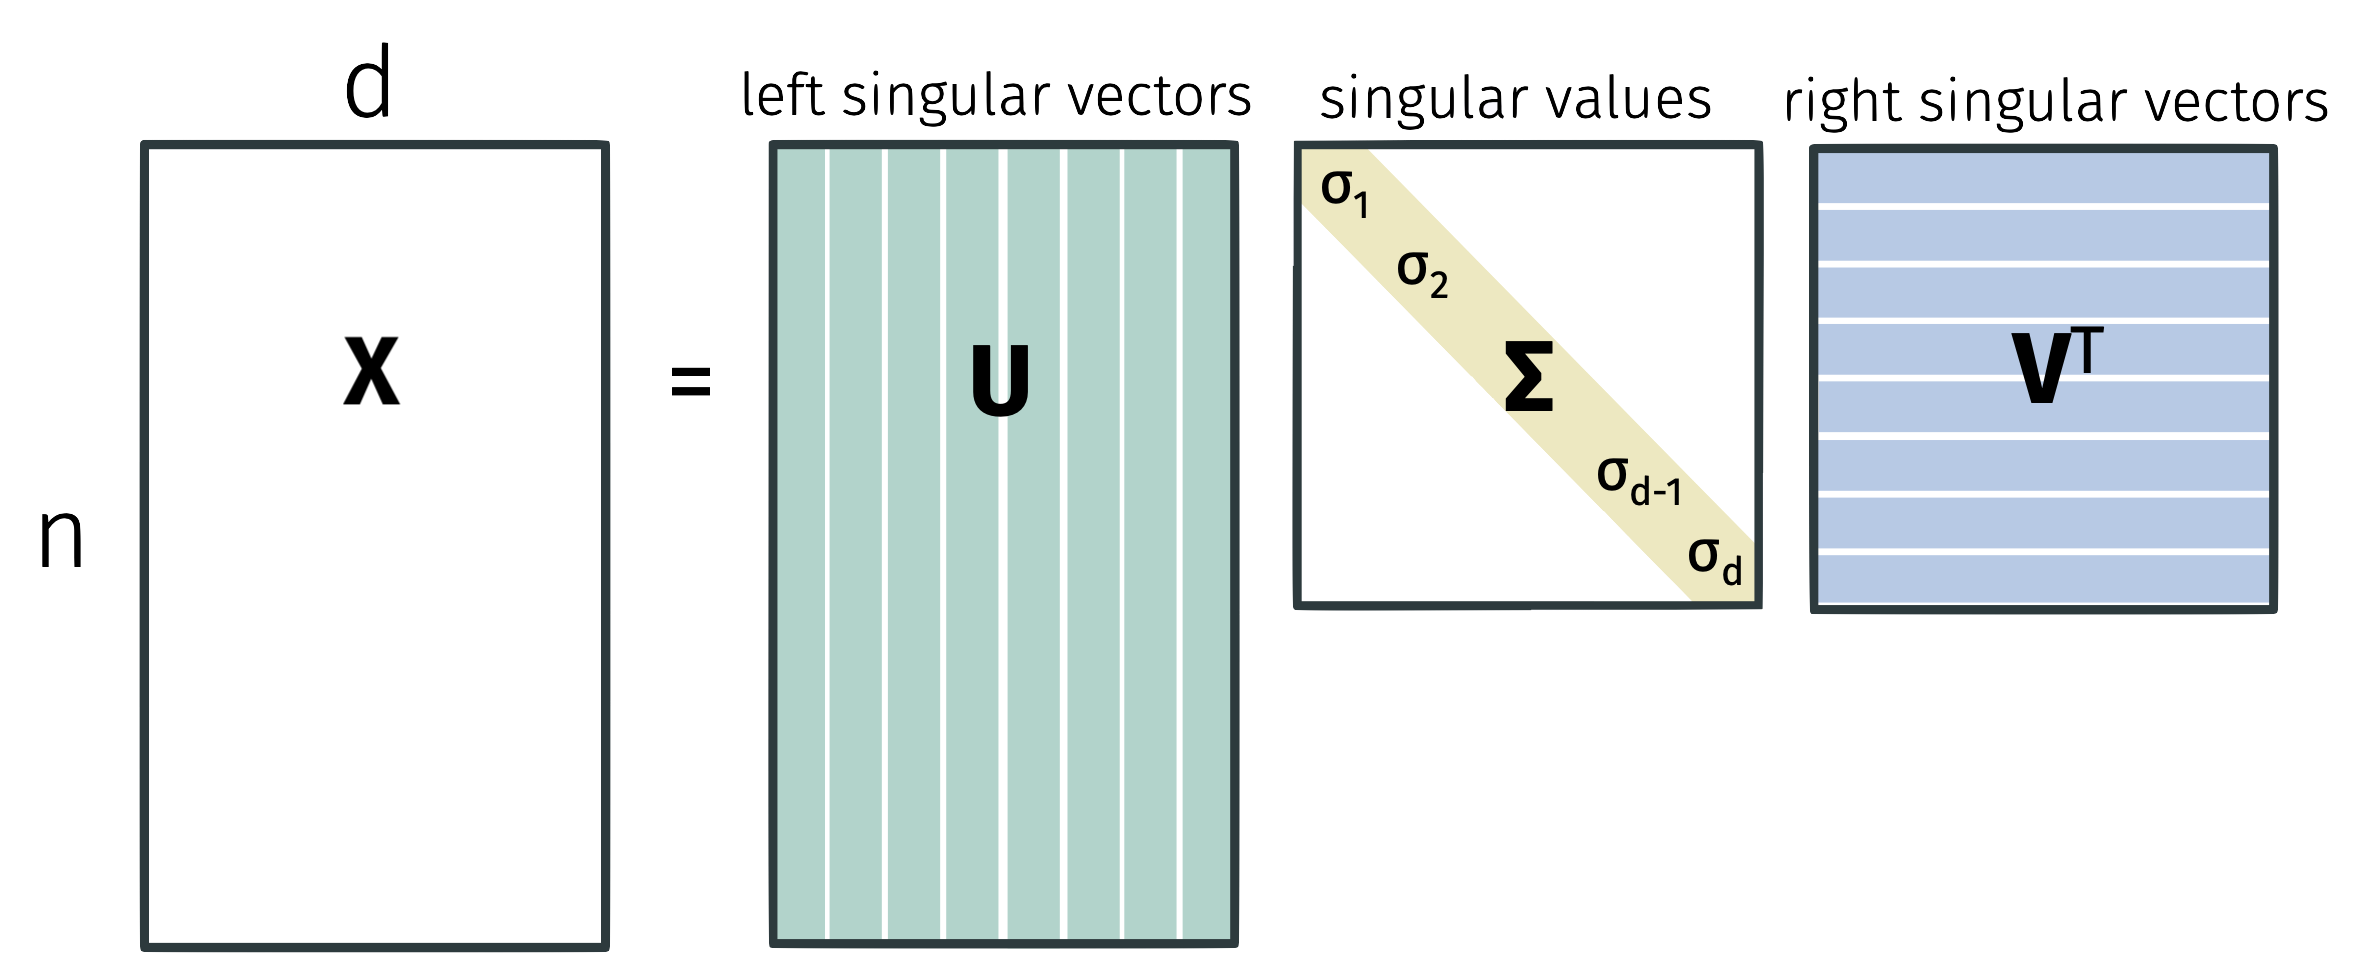
\includegraphics[width=.9\textwidth]{svd.png}
	\end{center} 
	Where $\bv{U}^T\bv{U} = \bv{I}$,  $\bv{V}^T\bv{V} = \bv{I}$, and $\sigma_1 \geq \sigma_2 \geq \ldots \sigma_d \geq 0$. 
	
Singular values are unique. Factors are not. E.g. would still get a valid SVD by multiplying both $i^\text{th}$ column of $\bv{V}$ and $\bv{U}$ by $-1$.
\end{frame}

\begin{frame}[t]
	\frametitle{important note for problem set}
	If $\bv{X}$ has rank $r \leq \min(n,d)$ it only have $r$ non-zero singular values. Some software packages will still return a full size $\bv{U}$ and $\bv{V}$ matrix. 
\vspace{-.5em}
	\begin{center}
		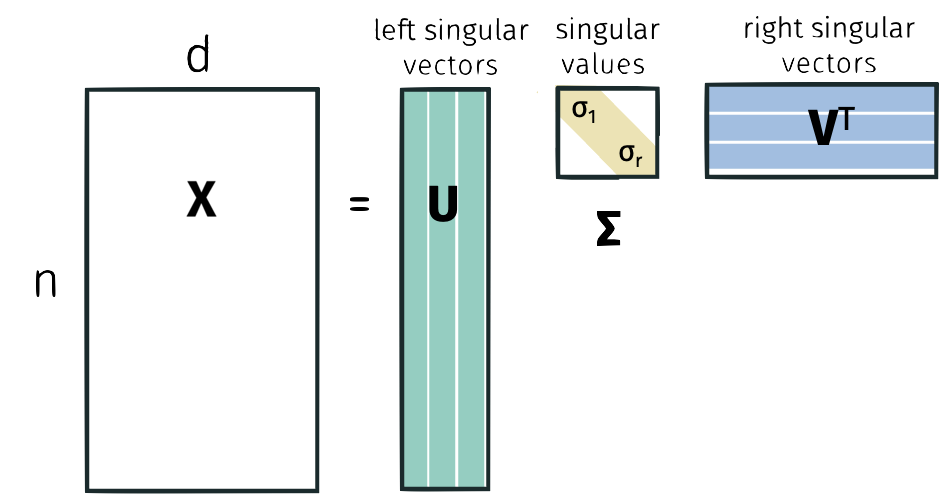
\includegraphics[width=.9\textwidth]{low_rank_a.png}
	\end{center} 
\end{frame}

\begin{frame}[t]
	\frametitle{other things to note}
	\begin{center}
		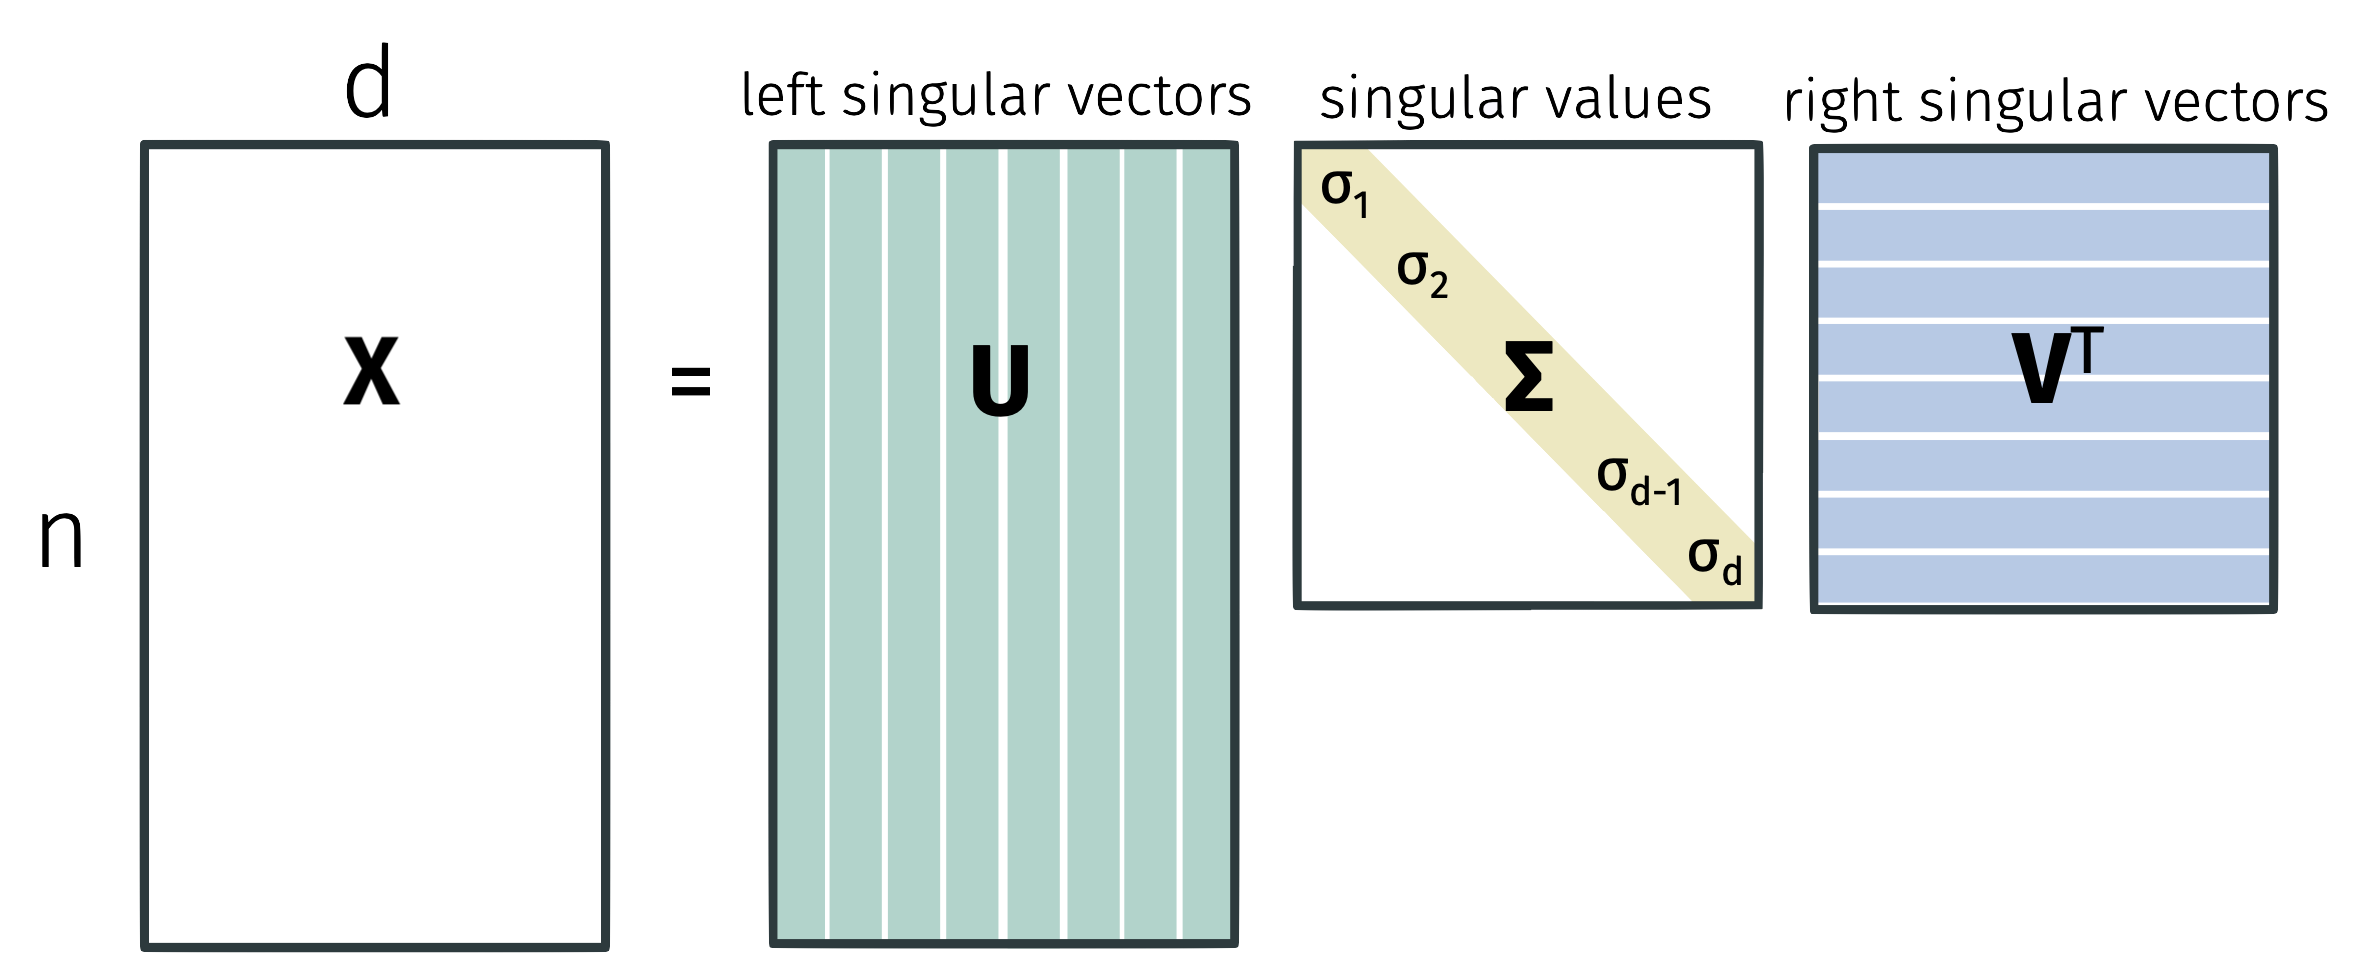
\includegraphics[width=.9\textwidth]{svd.png}
	\end{center} 
	\begin{align*}
		\|\bv{X}\|_F^2 = \sum_{i=1}^d \sigma_i^2
	\end{align*}
	\begin{align*}
		\|\bv{X}\|_2 = \sigma_1
	\end{align*}
\end{frame}

\begin{frame}
	\frametitle{low-rank approximation}
	Approximate $\bv{X}$ as the product of two rank $k$ matrices:
	\vspace{-1em}
	\begin{center}
		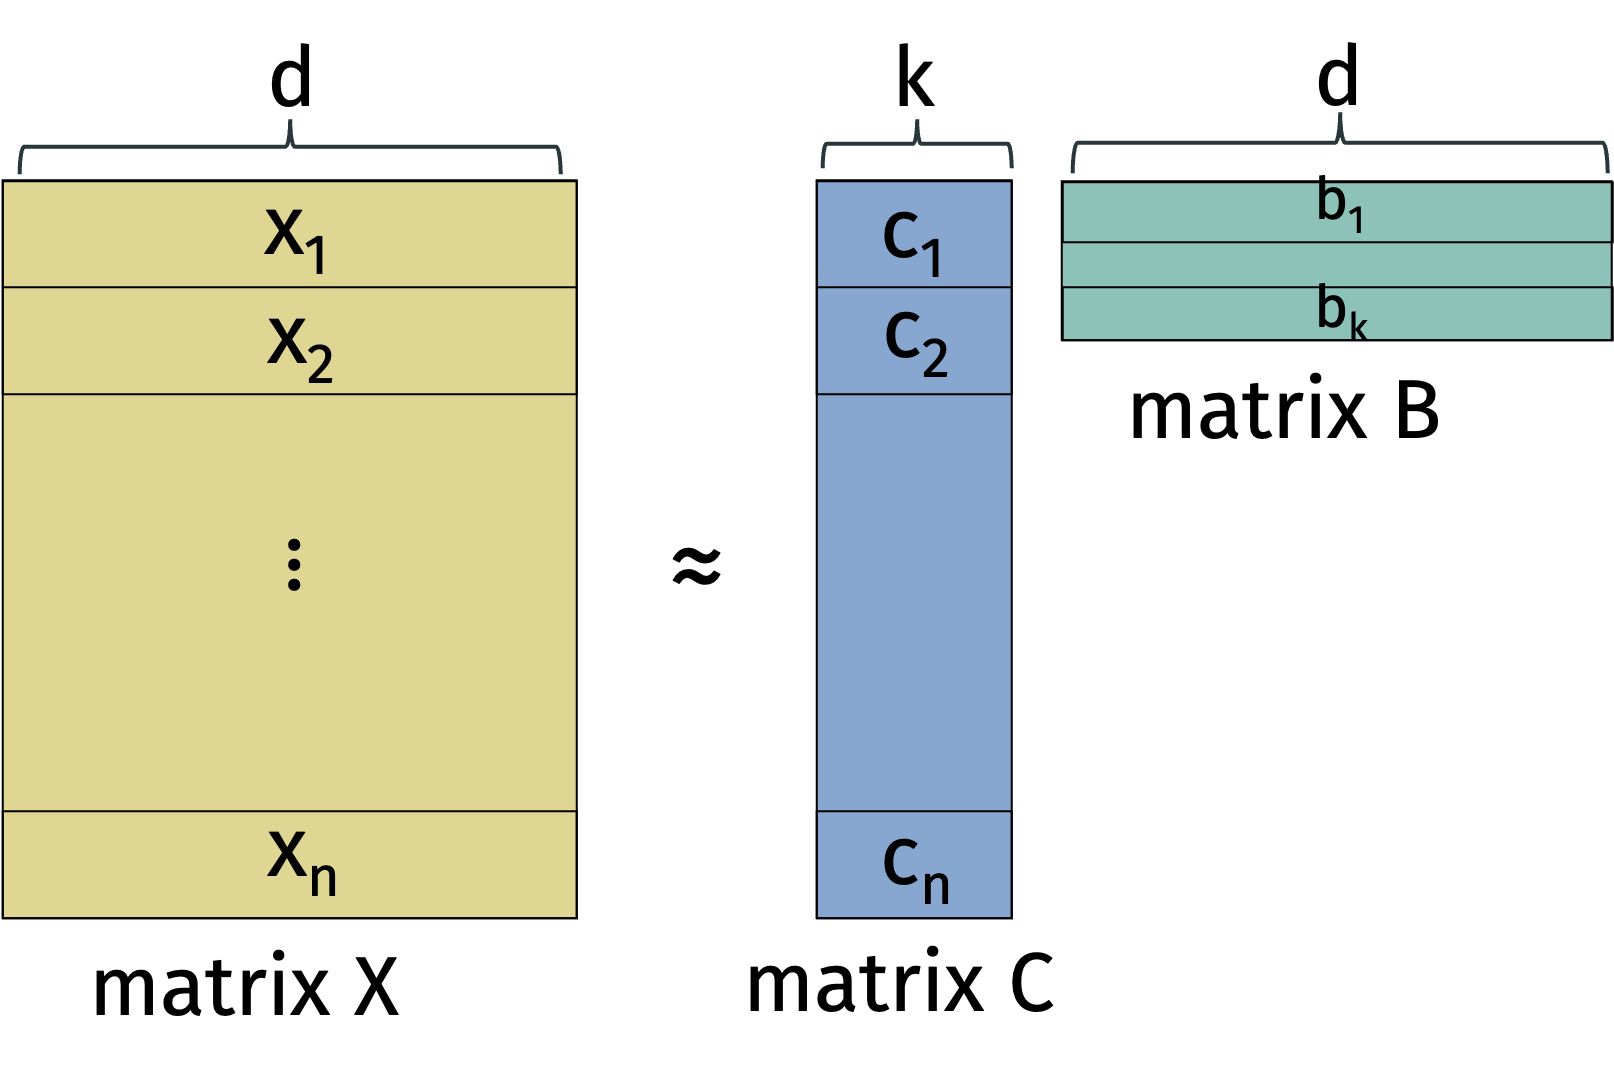
\includegraphics[width=.7\textwidth]{low-rank-basic.png}
	\end{center}
	\vspace{-.5em}
Typically choose $\bv{C}$ and $\bv{B}$ to minimize: 
\begin{align*}
	\min_{\bv{B},\bv{C}} \|\bv{X} - \bv{C}\bv{B}\|
\end{align*}
for some matrix norm. Common choice is $\|\bv{X} - \bv{C}\bv{B}\|_F^2$.
\end{frame}

\begin{frame}
	\frametitle{equivalent formulation}
	When measuring error with the Frobenius norm (or spectral norm) it suffices to find
	$d \times k$ orthogonal matrix $\bv{W}$ minimizing:
	\begin{align*}
		\|\bv{X} - \bv{X}\bv{W}\bv{W}^T\|_F
	\end{align*}
	\begin{center}
		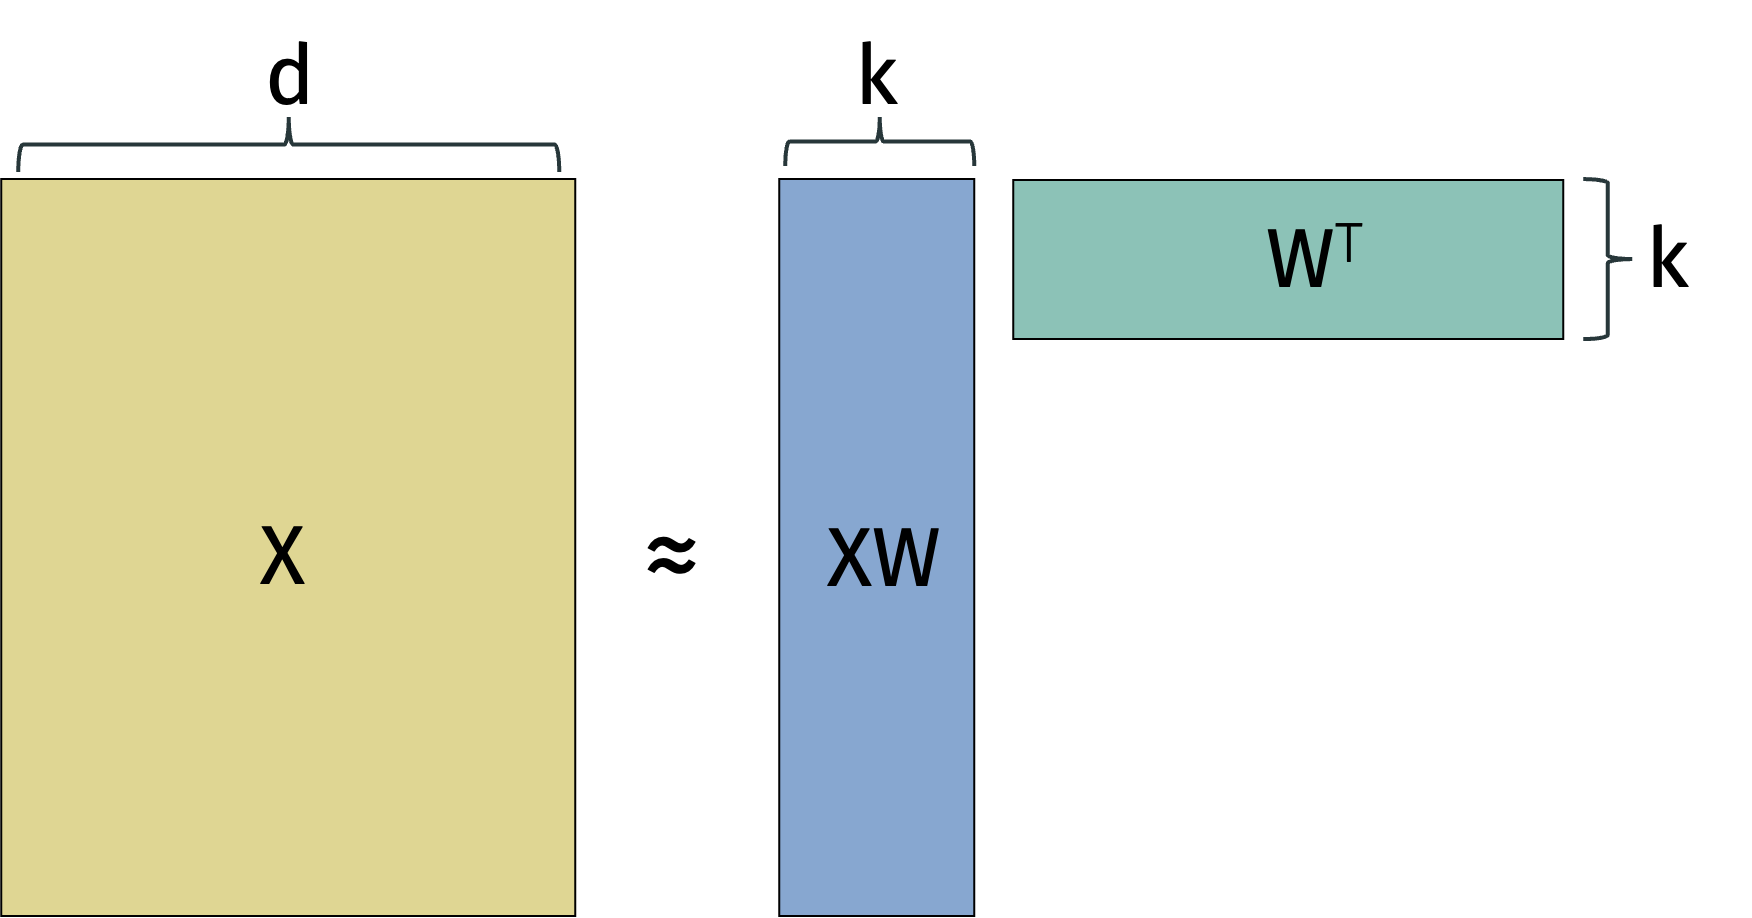
\includegraphics[width=.6\textwidth]{dualview.png}
	\end{center}
	I.e., best low-rank approximation \emph{projects} $\bv{X}$'s rows to a lower dimensional space.
\end{frame}

\begin{frame}
	\frametitle{equivalent formulation}
	Alternatively, suffices to find $n \times k$ orthogonal matrix $\bv{Z}$ minimizing:
	\begin{align*}
		\|\bv{X} - \bv{Z}\bv{Z}^T\bv{X}\|_F
	\end{align*}
\end{frame}

\begin{frame}
	\frametitle{why is data low-rank}
	\textbf{Row redundancy:} If a data set only had $k$ unique data points, it would be exactly rank $k$. If it has $k$ ``clusters'' of data points (e.g. the 10 digits) it's often very close to rank $k$. 
	\begin{center}
		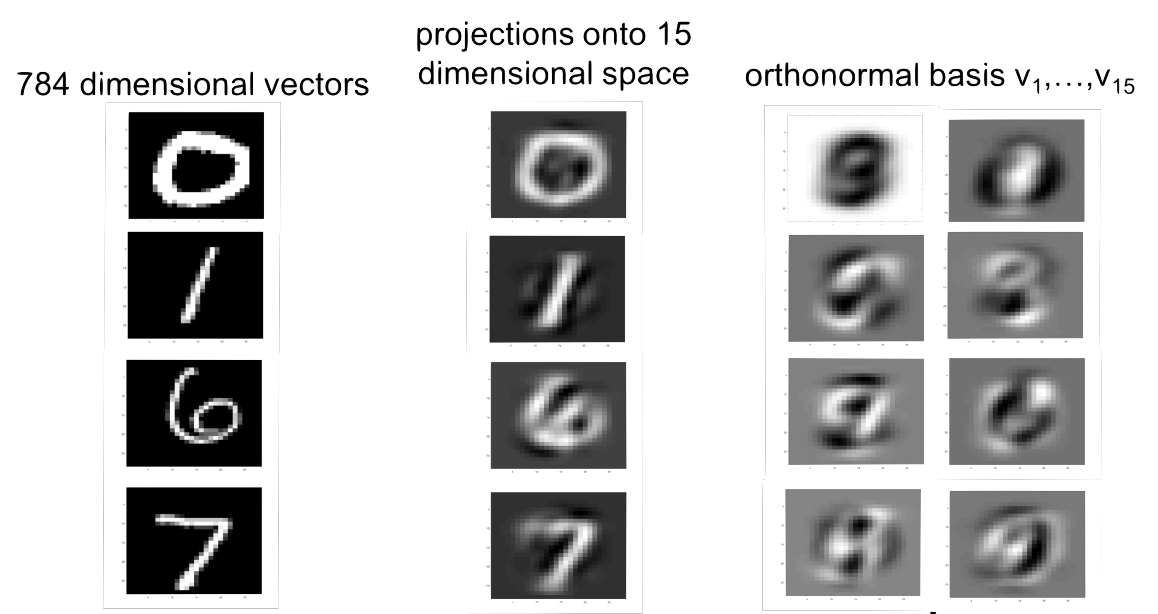
\includegraphics[width=.6\textwidth]{rowview.png}
	\end{center}
\end{frame}

\begin{frame}
	\frametitle{why is data low-rank}
	\textbf{Column redundancy:}
	Colinearity/correlation of data features leads to a low-rank data matrix. 
	\begin{center}
		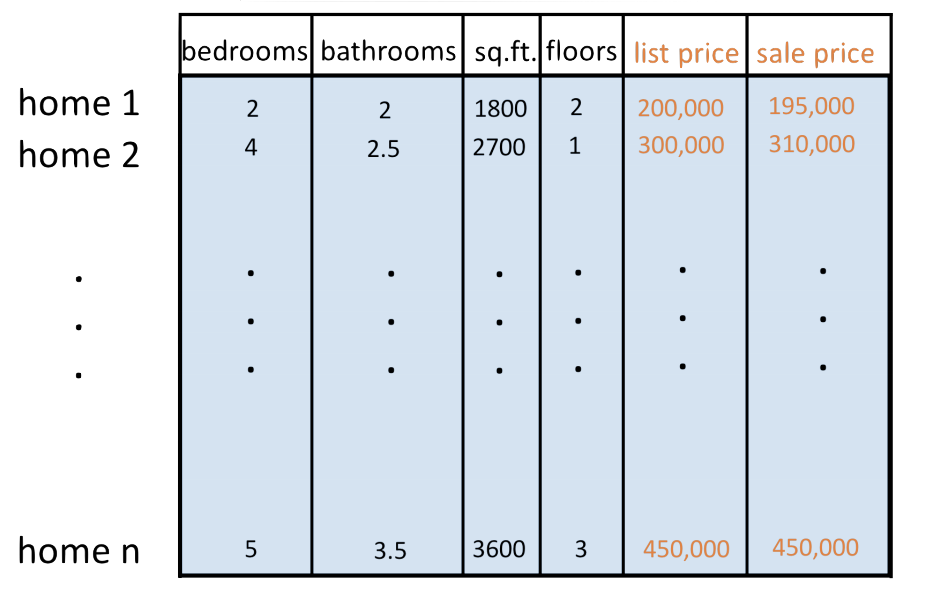
\includegraphics[width=.6\textwidth]{columnview.png}
	\end{center}
\end{frame}

\begin{frame}
	\frametitle{applications of low-rank approximation}
	Fact that $\|\bv{x}_i - \bv{x}_j\|_2 \approx \|\bv{x}_i^T\bv{WW}^T- \bv{x}_j^T\bv{WW}^T\|_2 = \|\bv{c}_i - \bv{c}_i\|_2$ leads to lots of applications.
	\begin{itemize}
		\item Data compression. E.g. used in state-of-the-art data dependent methods for nearest neighbor search.
		\item Data visualization when $k = 2$ or $3$. 
		\begin{center}
			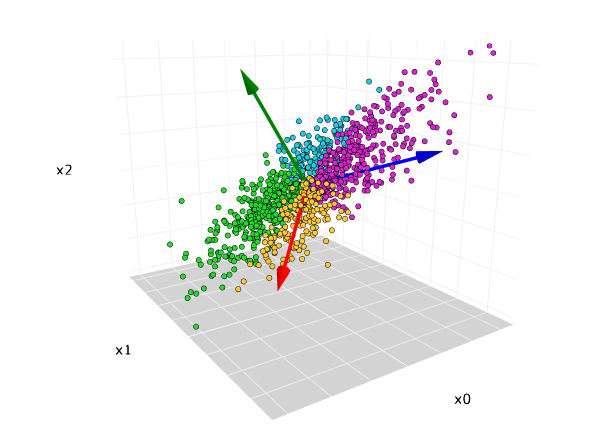
\includegraphics[width=.53\textwidth]{pca_vis.png}\hspace{1em} 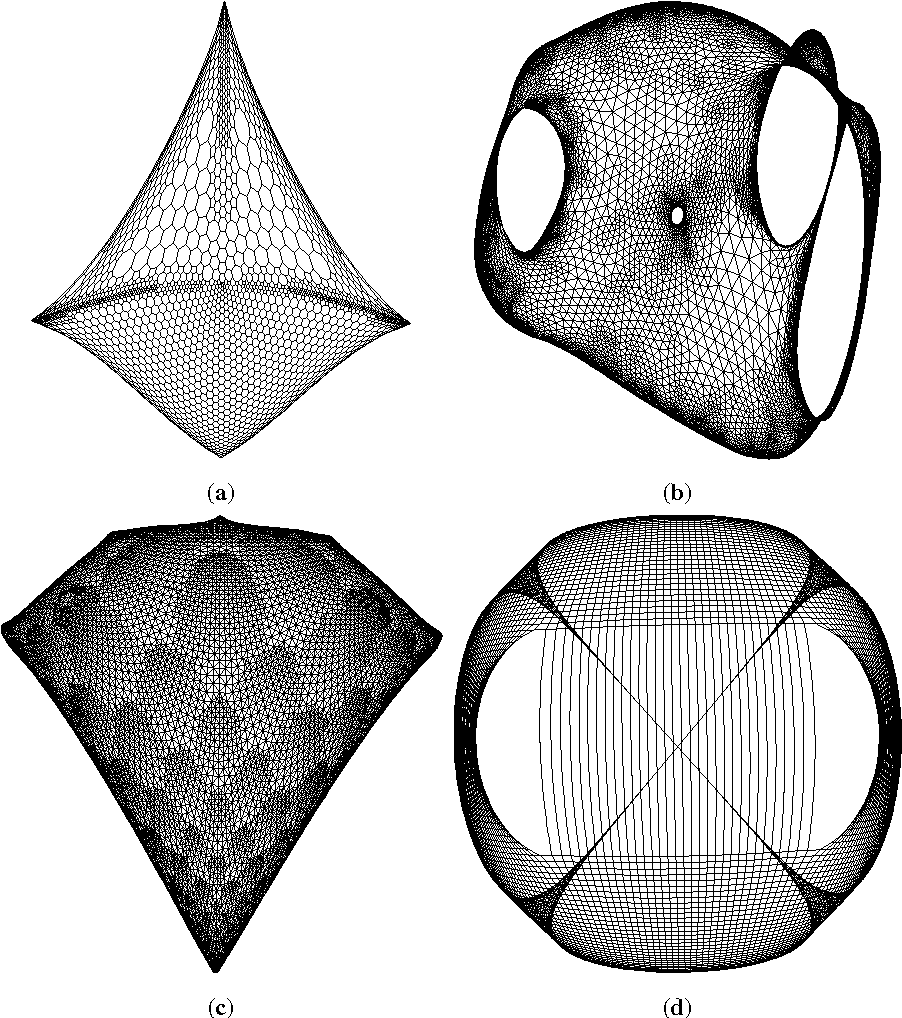
\includegraphics[width=.28\textwidth]{eigenvector_drawings.png}
		\end{center}
	\item  Data embeddings (e.g. word2vec, node2vec).
	\end{itemize}
\end{frame}

\begin{frame}
	\frametitle{applications of low-rank approximation}
		\begin{itemize}
		\item Reduced order modeling for solving physical equations.
		\begin{center}
			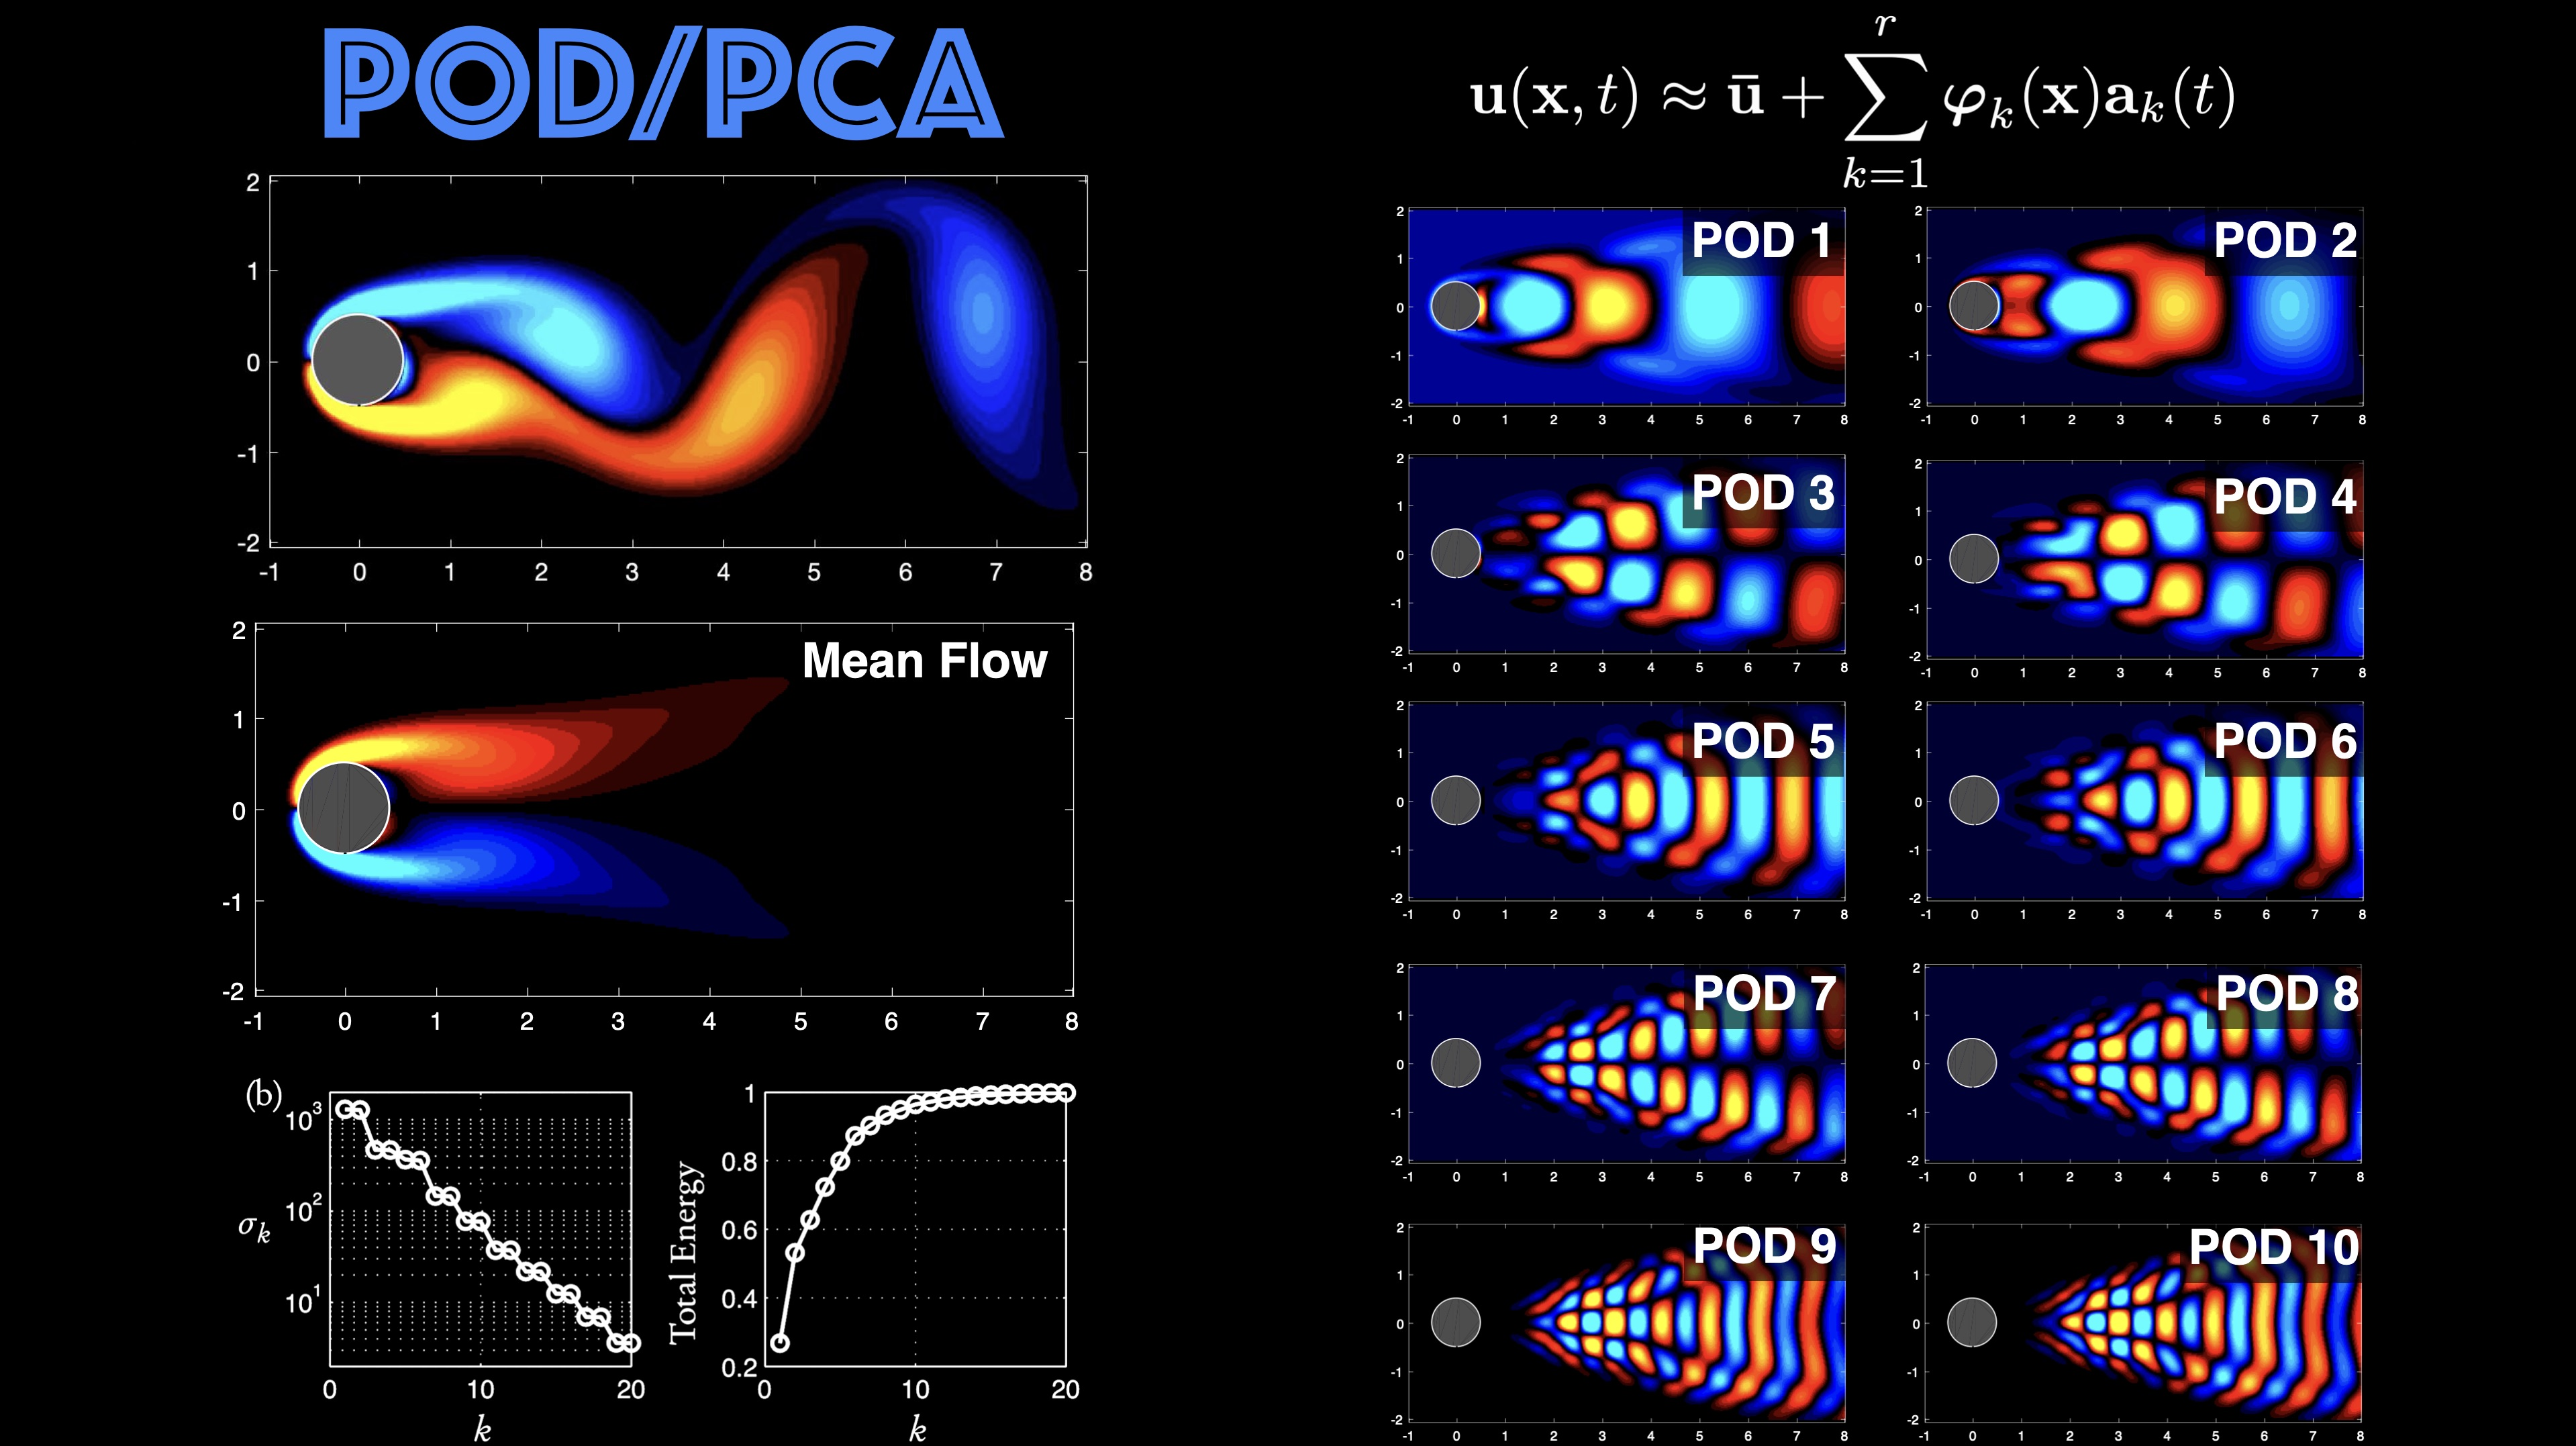
\includegraphics[width=.6\textwidth]{diffeq.jpg}
		\end{center}
		\item Constructing preconditioners in optimization.
		\item Noisy triangulation (on problem set).
	\end{itemize}
\end{frame}

\begin{frame}[t]
	\frametitle{partial svd}
	\textbf{Key result:} Can find the best projection from the singular value decomposition.
	\begin{center}
		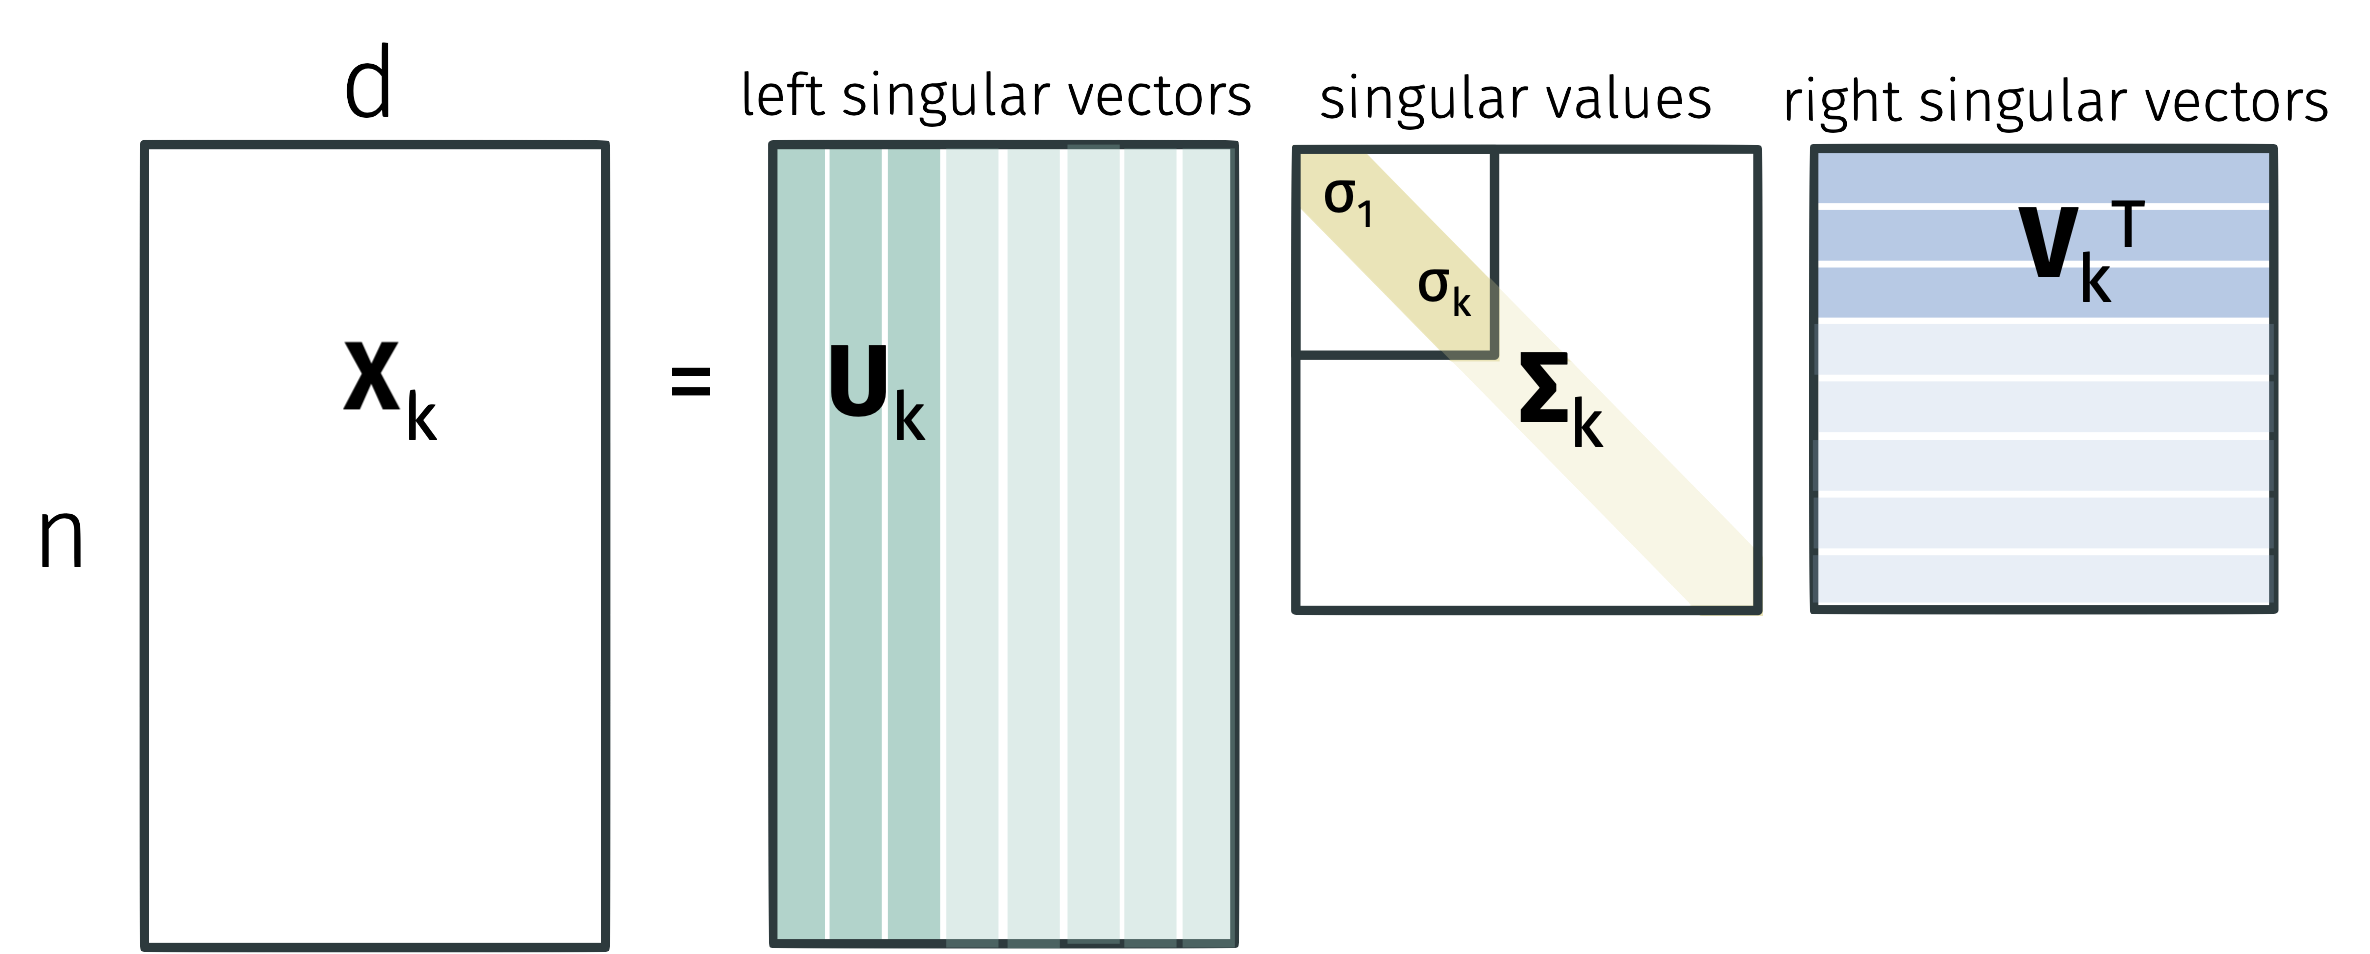
\includegraphics[width=.9\textwidth]{svdk.png}
	\end{center} 
	\begin{align*}
		\bv{U}_k = 	\argmin_{\text{orthogonal }\bv{Z} \in \R^{d\times k}} \|\bv{X} - \bv{Z}\bv{Z}^T\bv{X}\|_F^2
		\end{align*}
	\begin{align*}
	\bv{V}_k = 	\argmin_{\text{orthogonal }\bv{W} \in \R^{d\times k}} \|\bv{X} - \bv{X}\bv{W}\bv{W}^T\|_F^2
	\end{align*}
\end{frame}

\begin{frame}[t]
	\frametitle{optimal low-rank approximation}
	\textbf{Claim:} $\bv{X}_k = \bv{U}_k\bs{\Sigma}_k\bv{V}_k^T = \bv{U}_k\bv{U}_k^T\bv{X}  = \bv{X} \bv{V}_k\bv{V}_k^T$. 
\end{frame}

\begin{frame}[t]
	\frametitle{optimality of svd}
	\textbf{Claim 1:}
	\begin{align*}
		\argmin_{\text{rank $k$ }\bv{B}}  \|\bv{X} - \bv{B}\|_F^2 = \left[\argmin_{\text{rank $k$}\bv{B}}   \|\bv{U}\bs{\Sigma} -\bv{B}\|_F^2\right] \cdot\bv{V}^T
	\end{align*}

		\begin{center}
	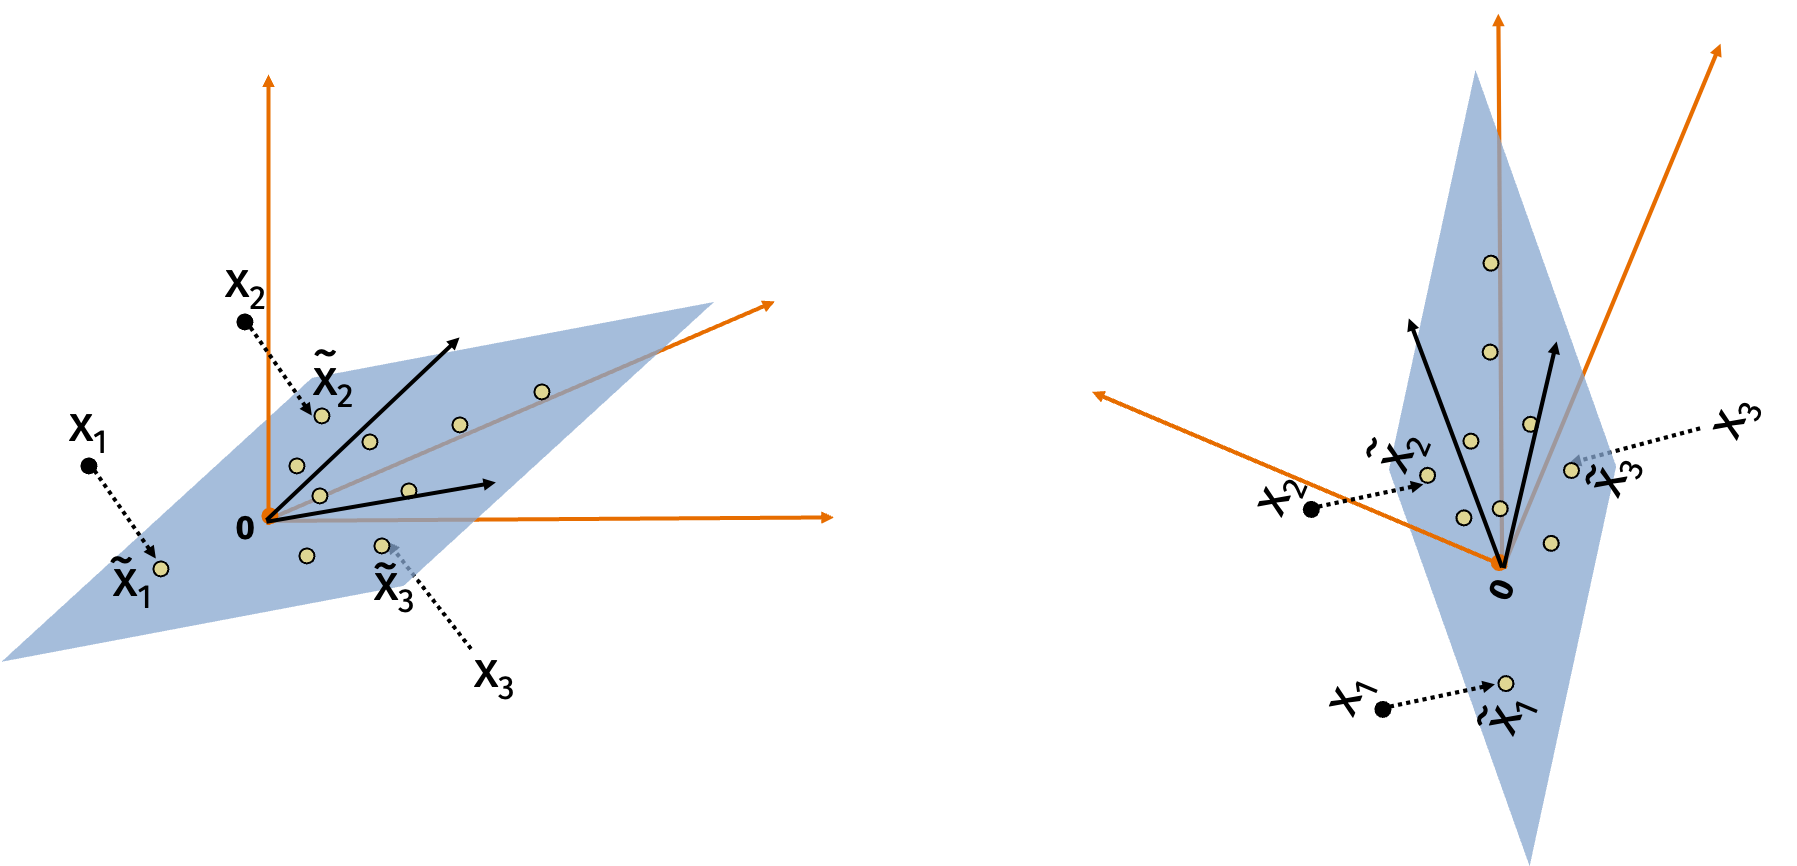
\includegraphics[width=.8\textwidth]{rotation_invariant.png}
\end{center} 
\end{frame}

\begin{frame}[t]
	\frametitle{optimality of svd}		
	\textbf{Claim 2:}
	\begin{align*}
		\argmin_{\text{rank $k$ }\bv{B}}  \|\bv{U}\bs{\Sigma} -  \bv{B}^T\|_F^2 = \argmin_{\text{rank $k$ }\bv{B}}  \|\bs{\Sigma} -  \bv{U}^T\bv{B}^T\|_F^2 
	\end{align*}

Choose $\bv{B}^T$ so that $\bv{U}^T\bv{B}^T$ is an optimal rank $k$ approximation of $\bs{\Sigma}$. I.e., $\bs{\Sigma}_k$.
\end{frame}

\begin{frame}[t]
	\frametitle{useful observations}
		\begin{center}
		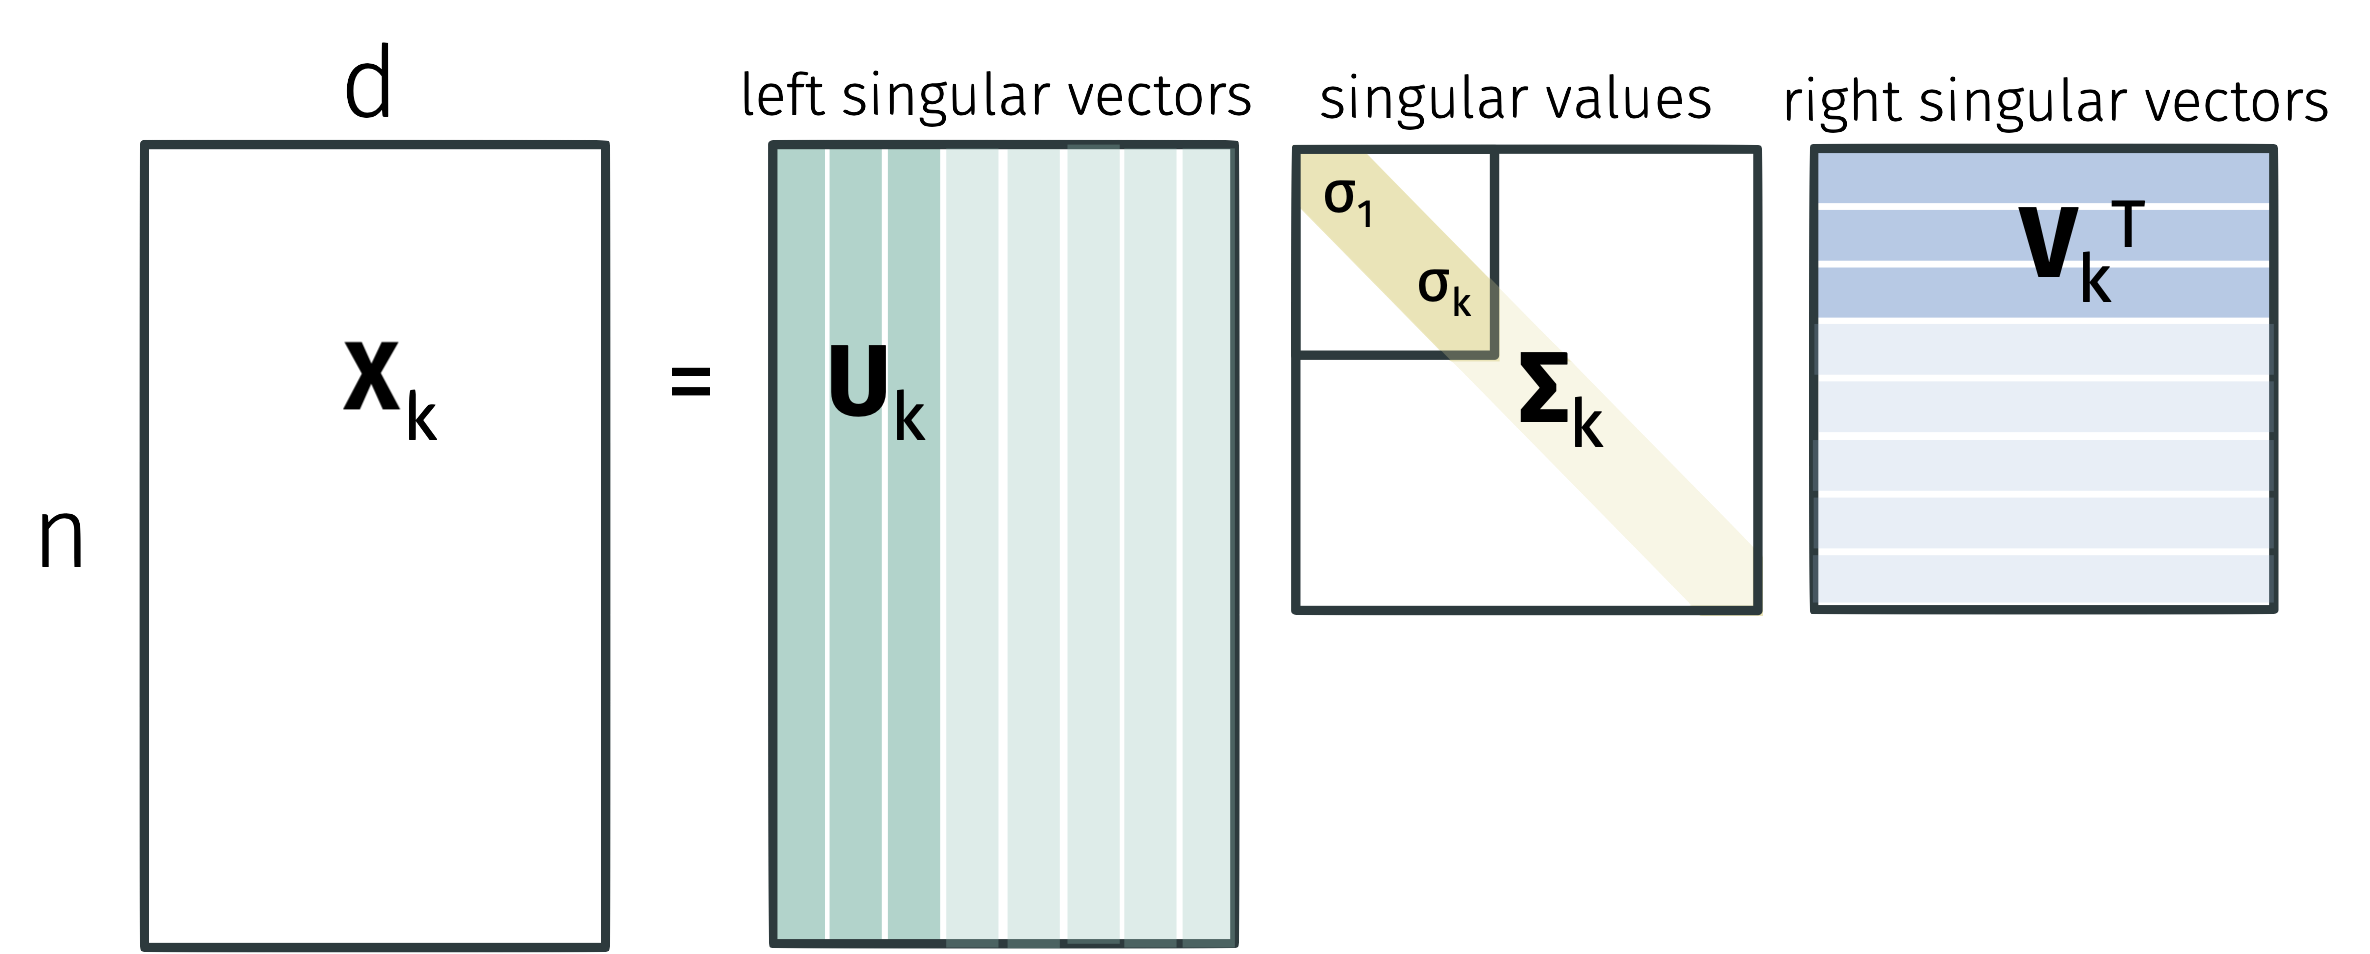
\includegraphics[width=.7\textwidth]{svdk.png}
	\end{center} 
\textbf{Observation 1:}
\begin{align*}
	\argmin_{\bv{W} \in \R^{d\times k}} \|\bv{X} - \bv{X}\bv{W}\bv{W}^T\|_F^2 = \argmax_{\bv{W} \in \R^{d\times k}} \|\bv{X}\bv{W}\bv{W}^T\|_F^2
\end{align*}
{Follows from fact that for \emph{all} orthogonal $\bv{W}$:}
\begin{align*}
	 \|\bv{X} - \bv{X}\bv{W}\bv{W}^T\|_F^2 =  \|\bv{X}\|_F^2 - \|\bv{X}\bv{W}\bv{W}^T\|_F^2
\end{align*} 
This is often the perspective people take when thinking about Principal Component Analysis. 
\end{frame}

\begin{frame}[t]
	\frametitle{useful observations}
	\textbf{Claim:}
	 \begin{align*}
		\|\bv{X} - \bv{X}\bv{W}\bv{W}^T\|_F^2 =  \|\bv{X}\|_F^2 - \|\bv{X}\bv{W}\bv{W}^T\|_F^2
	\end{align*} 
	\begin{center}
	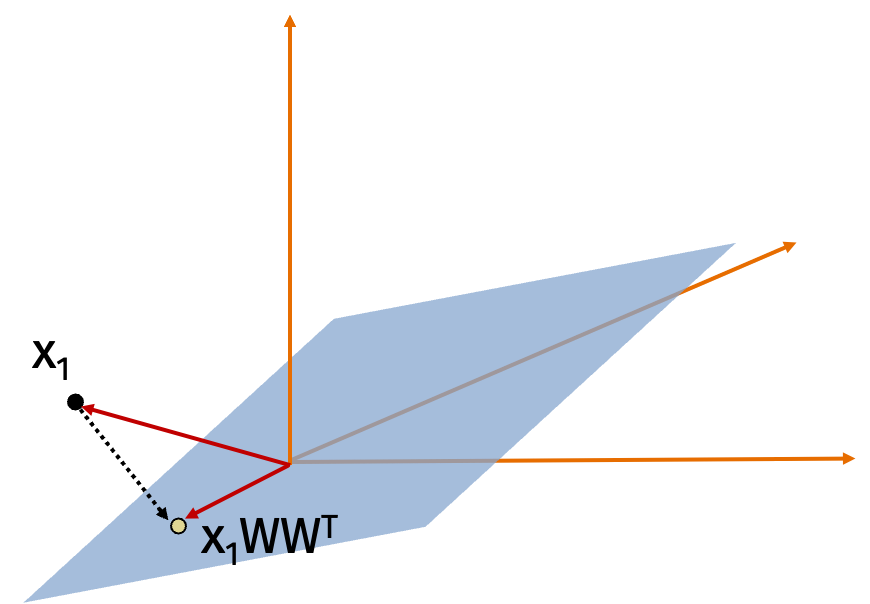
\includegraphics[width=.7\textwidth]{pythagorean.png}
\end{center} 
	
\end{frame}

\begin{frame}[t]
	\frametitle{useful observations}
	\begin{center}
		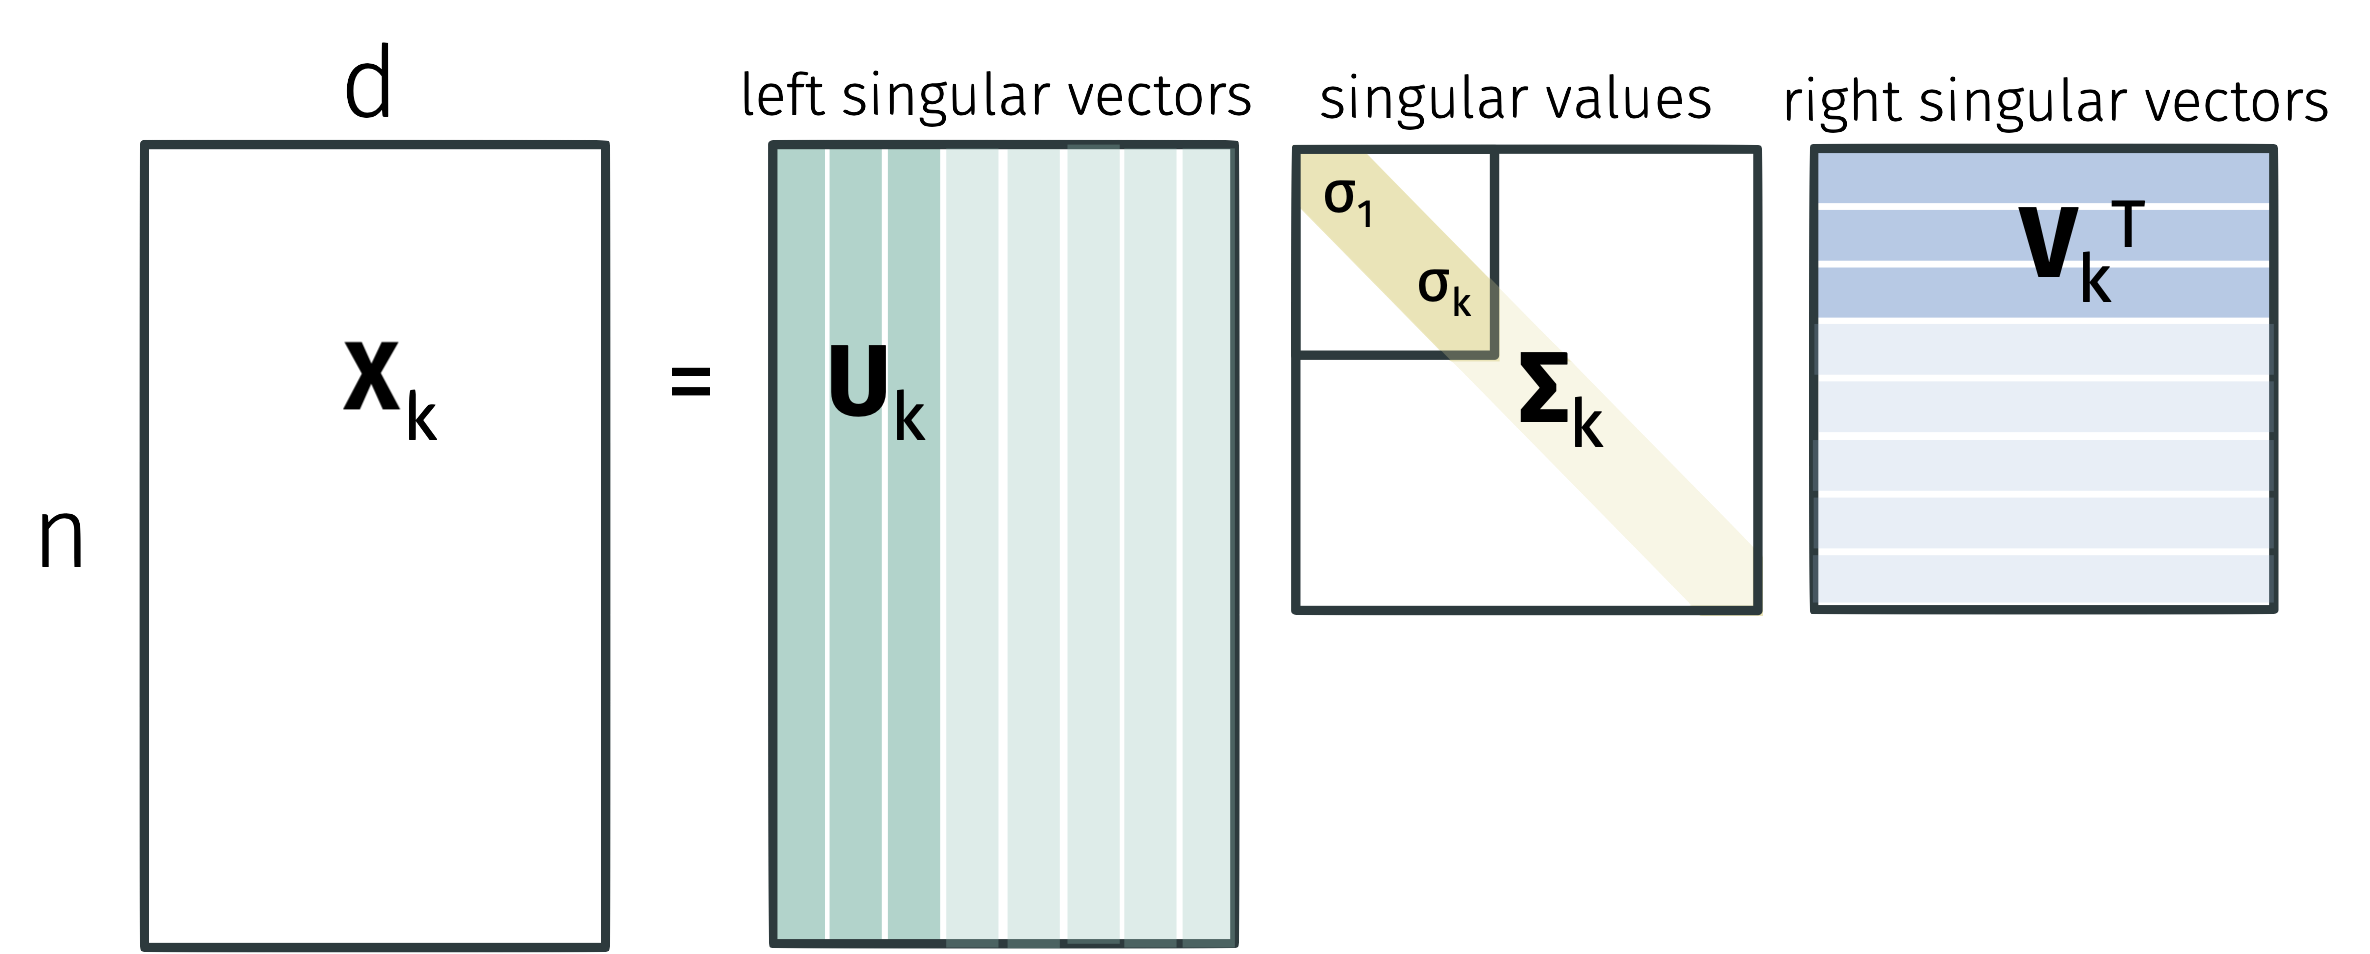
\includegraphics[width=.6\textwidth]{svdk.png}
	\end{center} 
	\textbf{Observation 2:}
	The optimal low-rank approximation error $E_k = \|\bv{X} - \bv{X}_k\|_F^2 = \|\bv{X}\|_F^2 - \|\bv{X}_k\|_F^2$ can be written:
	\begin{align*}
		E_k = \sum_{i=k+1}^d \sigma_i^2.
	\end{align*}
\end{frame}

\begin{frame}[t]
	\frametitle{spectral plots}
	\textbf{Observation 2:}
	The optimal low-rank approximation error $E_k = \|\bv{X} - \bv{X}_k\|_F^2 = \|\bv{X}\|_F^2 - \|\bv{X}_k\|_F^2$ can be written:
	\begin{align*}
	E_k = \sum_{i=k+1}^d \sigma_i^2.
	\end{align*}
	Can immediately get a sense of ``how low-rank'' a matrix is from it's spectrum:
	\begin{center}
		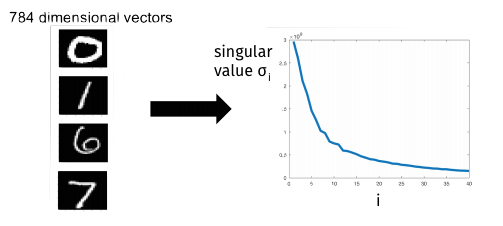
\includegraphics[width=.8\textwidth]{mnist_spectrum.png}
	\end{center}
\end{frame}

\begin{frame}[t]
	\frametitle{spectral plots}
	\textbf{Observation 2:}
	The optimal low-rank approximation error $E_k = \|\bv{X} - \bv{X}_k\|_F^2 = \|\bv{X}\|_F^2 - \|\bv{X}_k\|_F^2$ can be written:
	\begin{align*}
	E_k = \sum_{i=k+1}^d \sigma_i^2.
	\end{align*}
	Can immediately get a sense of ``how low-rank'' a matrix is from it's spectrum:
	\begin{center}
		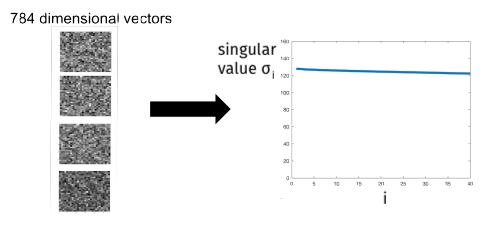
\includegraphics[width=.8\textwidth]{noise_spectrum.png}
	\end{center}
\end{frame}

\begin{frame}[t]
	\frametitle{spectral plots}
	\textbf{Observation 2:}
	The optimal low-rank approximation error $E_k = \|\bv{X} - \bv{X}_k\|_F^2 = \|\bv{X}\|_F^2 - \|\bv{X}_k\|_F^2$ can be written:
	\begin{align*}
	E_k = \sum_{i=k+1}^d \sigma_i^2.
	\end{align*}
	Can immediately get a sense of ``how low-rank'' a matrix is from it's spectrum:
	\begin{center}
		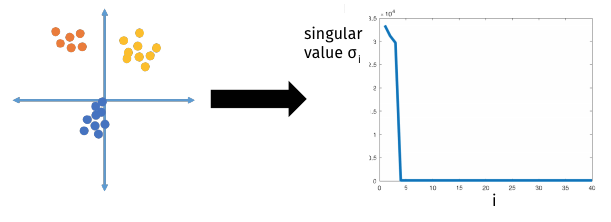
\includegraphics[width=.8\textwidth]{cluster_spectrum.png}
	\end{center}
\end{frame}

\begin{frame}[t]
	\frametitle{computing the svd}
	Suffices to compute right singular vectors $\bv{V}$:
	\begin{itemize}
		\item Compute $\bv{X}^T\bv{X}$.
		\item Find eigendecomposition $\bv{V}\bs{\Lambda}\bv{V}^T = \bv{X}^T\bv{X}$ using e.g. QR algorithm.
		\item Compute $\bv{L} = \bv{X}\bv{V}$. Set $\sigma_i = \|\bv{L}_i\|_2$ and $\bv{U}_i = \bv{L}_i/\|\bv{L}_i\|_2$.
	\end{itemize}

\vspace{2em}
\begin{center}
	\hspace{-3em} \alert{\textbf{Total runtime $\approx$}}
\end{center}
\end{frame}

\begin{frame}[t]
	\frametitle{computing the svd (faster)}
	\textbf{How to go faster?}
	\begin{itemize}
		\item Compute \emph{approximate} solution.
		\item Only compute \emph{top $k$ singular vectors/values}.
		\item \emph{Iterative algorithms} achieve runtime $\approx O(ndk)$ vs. $O(nd^2)$ time.  
		\begin{itemize}
			\item \textbf{Krylov subspace methods} like the Lanczos method are most commonly used in practice. 
			\item \textbf{Power method} is the simplest Krylov subspace method, and still works very well. 
		\end{itemize}
	\end{itemize}
\end{frame}

\begin{frame}[t]
	\frametitle{power method}
	\textbf{Today:} What about when $k = 1$? 
	
	\textbf{Goal:} Find some $\bv{z} \approx \bv{v}_1$. 
	
	\textbf{Input:} $\bv{X} \in \R^{n\times d}$ with SVD $\bv{U}\bs{\Sigma}\bv{V}^T$. 
%	\textbf{Parameter:} Let $\gamma = \frac{\sigma_1 - \sigma_2}{\sigma_1}$.
	
	\vspace{2em}
	\textbf{Power method:}
	\begin{itemize}
		\item Choose $\bv{z}^{(0)}$ randomly. $\bv{z}_0 \sim \mathcal{N}(0,1)$.
		\item $\bv{z}^{(0)} = \bv{z}^{(0)} /\|\bv{z}^{(0)}\|_2$
		\item For $i = 1,\ldots, T$
		\begin{itemize}
			\item $\bv{z}^{(i)} = \bv{X}^T\cdot(\bv{X}\bv{z}^{(i-1)} )$
			\item $n_i = \|\bv{z}^{(i)}\|_2$
			\item $\bv{z}^{(i)}  = \bv{z}^{(i)} /n_i$
		\end{itemize}
	Return $\bv{z}^{(T)}$
	\end{itemize} 
\end{frame}

\begin{frame}[t]
	\frametitle{power method intuition}
	\begin{center}
		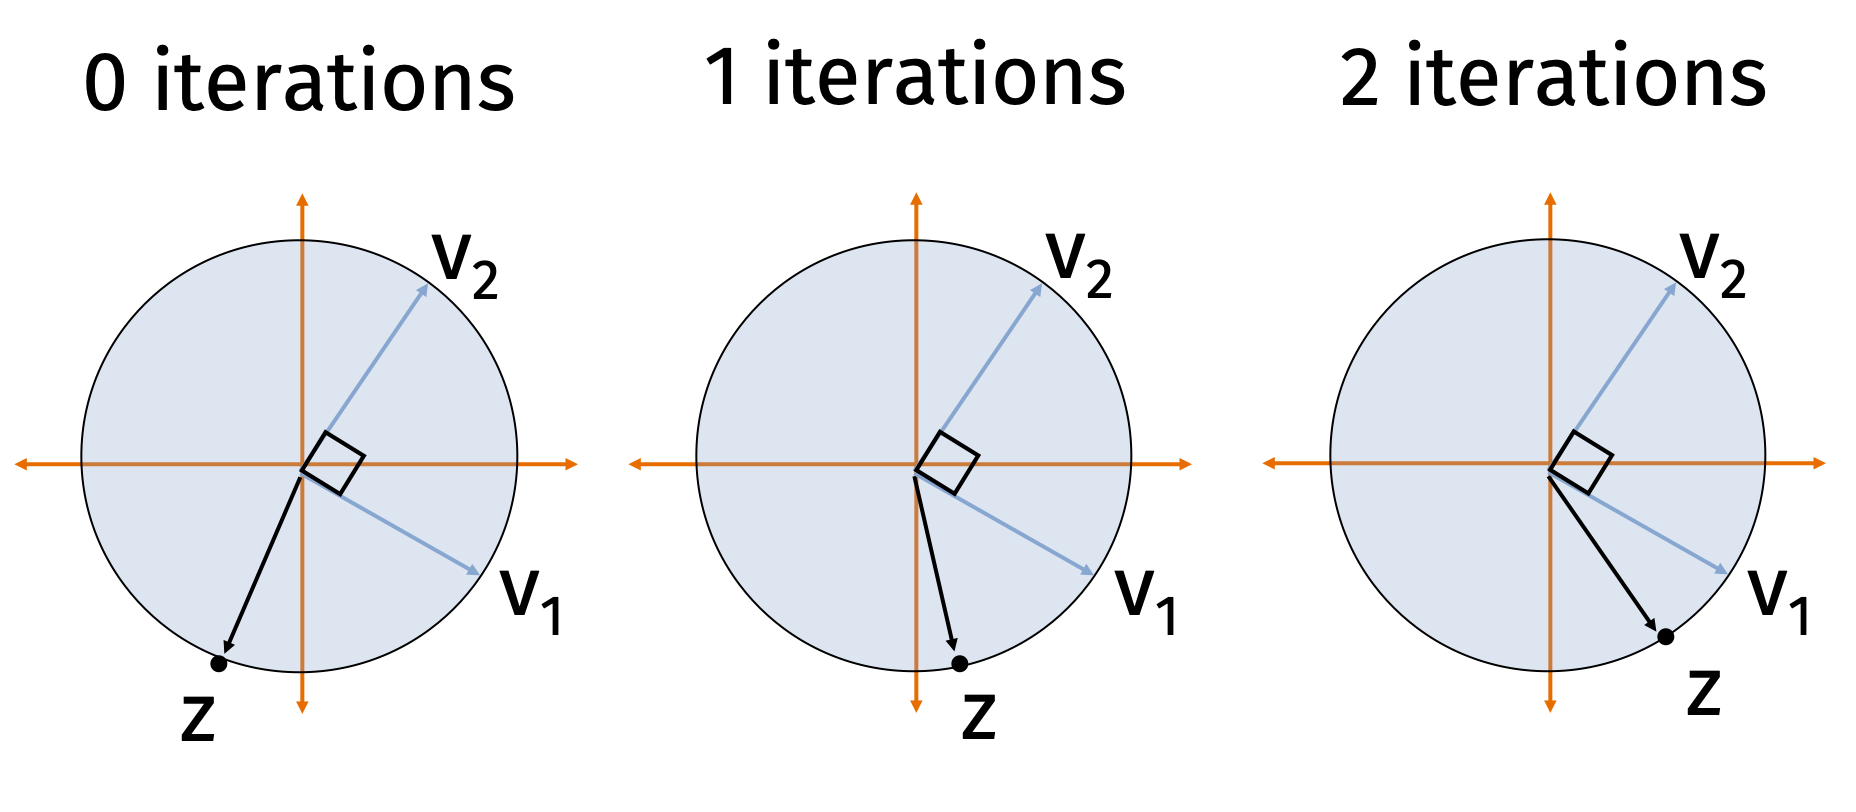
\includegraphics[width=\textwidth]{intuition.png}
	\end{center}
	
\end{frame}

\begin{frame}[t]
	\frametitle{power method formal convergence}	
	\begin{theorem}[Basic Power Method Convergence]
		Let $\gamma = \frac{\sigma_1 - \sigma_2}{\sigma_1}$ be  parameter capturing the ``gap'' between the first and second largest singular values. If Power Method is initialized with a random Gaussian vector then, with high probability, after $T = O\left(\frac{\log d/\epsilon}{\gamma}\right)$ steps, we have either:
		\begin{align*}
			\|\bv{v}_1 - \bv{z}^{(T)}\|_2 &\leq \epsilon &&\text{ or } &\|\bv{v}_1 - (-\bv{z}^{(T)})\|_2 &\leq \epsilon.
		\end{align*}
	\end{theorem}
	\alert{\textbf{Total runtime:}} $O\left(nd \cdot \frac{\log d/\epsilon}{\gamma}\right)$
\end{frame}

\begin{frame}[t]
	\frametitle{one step analysis of power method}
	Write $\bv{z}^{(i)}$ in the right singular vector basis:
	\begin{align*}
		\bv{z}^{(0)} &= c_1^{(0)}\bv{v}_1 + {c}_2^{(0)}\bv{v}_2 + \ldots + c_d^{(0)} \bv{v}_d \\
		\bv{z}^{(1)} &= c_1^{(1)}\bv{v}_1 + {c}_2^{(1)}\bv{v}_2 + \ldots + c_d^{(1)} \bv{v}_d\\
		\vdots&\\
		\bv{z}^{(i)} &= c_1^{(i)}\bv{v}_1 + {c}_2^{(i)}\bv{v}_2 + \ldots + c_d^{(i)} \bv{v}_d\\
	\end{align*}
	
	\textbf{Note:} $[c_1^{(i)}, \ldots, c_d^{(i)}] = \bv{c}^{(i)} = \bv{V^T}\bv{z}^{(i)}$.
	
	\textbf{Also:} Since $\bv{V}$ is orthogonal and $\|\bv{z}^{(i)}\|_2 = 1$, $\|\bv{c}^{(i)}\|_2^2 = 1$. 
\end{frame}

\begin{frame}[t]
	\frametitle{one step analysis of power method}
	\textbf{Claim:} After update $\bv{z}^{(i)} =  \frac{1}{n_i}\bv{X}^T\bv{X}\bv{z}^{(i-1)}$,
	\begin{align*}
		c_j^{(i)} =  \frac{1}{n_i}\sigma_j^2 c_j^{(i-1)}
	\end{align*}
\vspace{-.5em}
	\begin{align*}
		\bv{z}^{(i)} = \frac{1}{n_i}\left[ c_1^{(i-1)}\alert{\sigma_1^2}\cdot\bv{v}_1 + {c}_2^{(i-1)} \alert{\sigma_2^2}\cdot\bv{v}_2 + \ldots + c_d^{(i-1)} \alert{\sigma_d^2} \cdot\bv{v}_d\right]
	\end{align*}
\textbf{Equivalently:} $\bv{c}^{(i)}= \frac{1}{n_i}\bs{\Sigma}^2\bv{c}^{(i-1)}.$
\end{frame}

\begin{frame}[t]
	\frametitle{multi-step analysis of power method}
	\textbf{Claim:} After $T$ updates:
	\begin{align*}
	\bv{z}^{(T)} = \frac{1}{\prod_{i=1}^T n_i} \left[ c_1^{(0)}\alert{\sigma_1^{2T}}\cdot \bv{v}_1 + c_2^{(0)} \alert{\sigma_2^{2T}}\cdot \bv{v}_2 + \ldots + c_d^{(0)} \alert{\sigma_d^{2T}}\cdot \bv{v}_d \right]
	\end{align*}


\vspace{10em}

Let $\alpha_j = \frac{1}{\prod_{i=1}^T n_i}c_j^{(0)}\alert{\sigma_j^{2T}}$. 
\textbf{Goal:} Show that $\alpha_j \ll \alpha_1$ for all $j\neq 1$. 
\end{frame}

\begin{frame}[t]
	\frametitle{power method formal convergence}	
	Since $\bv{z}^{(T)}$ is a unit vector, $\sum_{i=1}^d \alpha_i^2 = 1$. So $|\alpha_1| \leq 1$. 
	
	If we can prove that \alert{$\left| \frac{\alpha_j}{\alpha_1}\right| \leq \sqrt{\frac{\epsilon}{2d}}$} then we will have that \alert{$\|\bv{v}_1 - \bv{z}^{(T)}\|_2^2 \leq \epsilon$}.
	\begin{align*}
		\alpha_j^2 &\leq \alpha_1^2 \cdot \frac{\epsilon}{2d}\\
		1 = \alpha_1^2 + \sum_{j=2}^d \alpha_d^2&\leq \alpha_1^2 + \frac{\epsilon}{2}\\
		 \alpha_1^2 &\geq 1-\frac{\epsilon}{2} \\
		 \alert{|\alpha_1|} &\geq \alert{1-\frac{\epsilon}{2}}
	\end{align*}

\begin{align*}
	\|\bv{v}_1 - \bv{z}^{(T)}\|_2^2 = 2 - 2\langle\bv{v}_1,\bv{z}^{(T)}\rangle \leq \epsilon
\end{align*}
	
	
\end{frame}
\begin{frame}[t]
	\frametitle{power method formal convergence}
	Let's see how many steps $T$ it takes to ensure that \alert{$\left|\frac{\alpha_j}{\alpha_1}\right| \leq \sqrt{\frac{\epsilon}{2d}}$} where $\alpha_j = \frac{1}{\prod_{i=1}^T n_i}c_j^{(0)}{\sigma_j^{2T}}$
	
	\textbf{Assumption:} Starting coefficient on first eigenvector is not too small:\vspace{-.5em}
	\begin{align*}
		\left| c_1^{(0)}\right| \geq   O\left(\frac{1}{\sqrt{d}}\right). 
	\end{align*}
	We will prove shortly that it holds with probability $99/100$.
	
	\begin{align*}
		\frac{|\alpha_j|}{|\alpha_1|} = \frac{\sigma_j^{2T}}{\sigma_1^{2T}} \cdot \frac{|c_j^{(0)}|}{|c_1^{(0)}|} \leq \hspace{20em}
	\end{align*}
	
	\begin{align*}
		\text{Need } T = \hspace{10em}
	\end{align*}
\end{frame}

\begin{frame}[t]
		\frametitle{starting coefficient analysis}
	\textbf{Need to prove:} Starting coefficient on first eigenvector is not too small. I.e., with probability $99/100$,
	\begin{align*}
		\left| c_1^{(0)}\right| \geq   O\left(\frac{1}{\sqrt{d}}\right). 
	\end{align*}
	
	\textbf{Prove using Gaussian \emph{anti}-concentration.}
	First use rotational invariance of Gaussian:
	\vspace{-.5em}
	\begin{align*}
		\bv{c}^{(0)} = \frac{\bv{V}^T \bv{z}^{(0)}}{\| \bv{z}^{(0)}\|_2} =  \frac{\bv{V}^T \bv{z}^{(0)}}{\| \bv{V}^T\bv{z}^{(0)}\|_2} \sim \frac{\bv{g}}{\| \bv{g}\|_2}, 
	\end{align*}
	where $\bv{g} \sim \mathcal{N}(0,1)^d$.
\end{frame}

\begin{frame}[t]
	\frametitle{starting coefficient analysis}
	Need to show that with high probability, first entry of $\frac{\bv{g}}{\| \bv{g}\|_2} \geq c\cdot \frac{1}{\sqrt{d}}$. 
	
	\textbf{Part 1:}
	With super high probability (e.g. $99/100$), 
	\begin{align*}
		\|\bv{g}\|_2^2 \leq 
	\end{align*}
\end{frame}

\begin{frame}[t]
	\frametitle{starting coefficient analysis}
	Need to show that with high probability, the magnitude of the first entry of ${\bv{g}} \geq c$ for a constant $c$. Think e.g. $c = 1/10$.
	
	\textbf{Part 2:}
	With probablility $1 - O(\alpha)$,
	\begin{align*}
		|{g}_1| \geq  \alpha.
	\end{align*}
\vspace{-1em}

	\begin{center}
		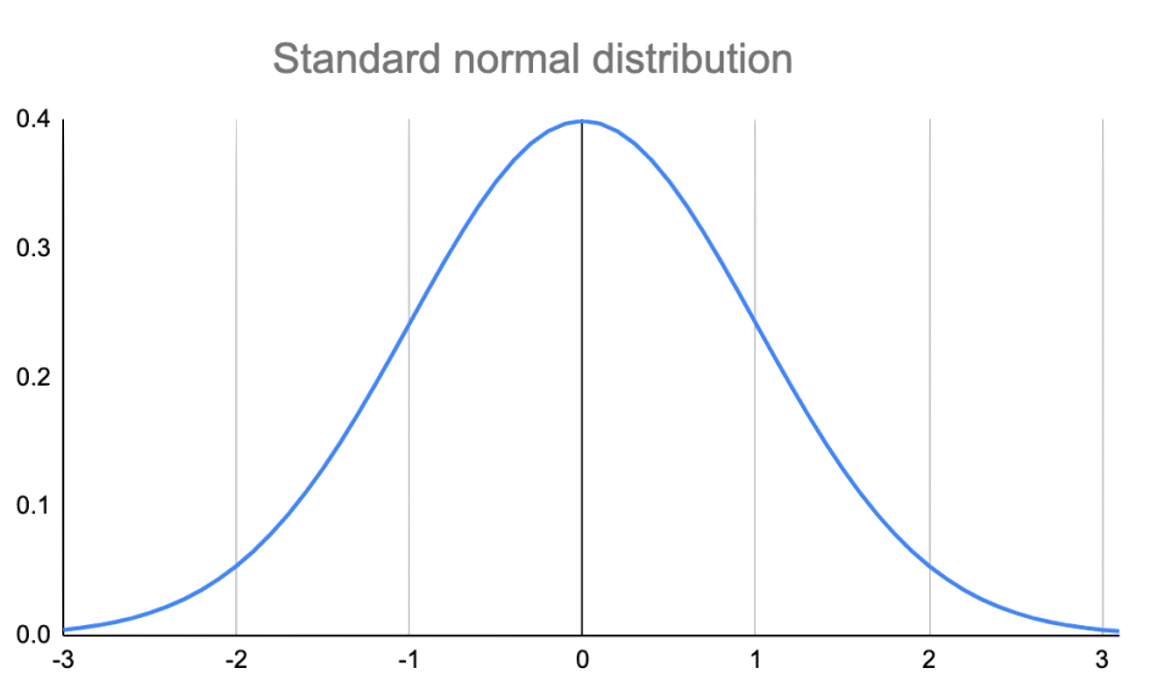
\includegraphics[width=.6\textwidth]{basic_gauss.png}
	\end{center}
\end{frame}

\begin{frame}[t]
	\frametitle{power method formal convergence}	
	\begin{theorem}[Basic Power Method Convergence]
		Let $\gamma = \frac{\sigma_1 - \sigma_2}{\sigma_1}$ be  parameter capturing the ``gap'' between the first and second largest singular values. If Power Method is initialized with a random Gaussian vector then, with high probability, after $T = O\left(\frac{\log d/\epsilon}{\gamma}\right)$ steps, we have either:
		\begin{align*}
			\|\bv{v}_1 - \bv{z}^{(T)}\|_2 &\leq \epsilon &&\text{ or } &\|\bv{v}_1 - (-\bv{z}^{(T)})\|_2 &\leq \epsilon.
		\end{align*}
	\end{theorem}
	The method truly won't converge if $\gamma$ is very small. Consider extreme case when $\gamma = 0$.
	\begin{align*}
		\bv{z}^{(T)} = \frac{1}{\prod_{i=1}^T n_i} \left[ c_1^{(0)}\alert{\sigma_1^{2T}}\cdot \bv{v}_1 + c_2^{(0)} \alert{\sigma_2^{2T}}\cdot \bv{v}_2 + \ldots + c_d^{(0)} \alert{\sigma_d^{2T}}\cdot \bv{v}_d \right]
	\end{align*}
\end{frame}

\begin{frame}[t]
	\frametitle{power method -- no gap dependence}	
	\begin{theorem}[Gapless Power Method Convergence]
		 If Power Method is initialized with a random Gaussian vector then, with high probability, after $T = O\left(\frac{\log d/\epsilon}{\epsilon}\right)$ steps, we obtain a $\bv{z}$ satisfying:
		\begin{align*}
		\|\bv{X} - \bv{X}\bv{z}\bv{z}^{T}\|_F^2 \leq (1+\epsilon)\|\bv{X} - \bv{X}\bv{v}_1\bv{v}_1^T\|_F^2 
		\end{align*}
	\end{theorem}	
\textbf{Intuition:} For a good low-rank approximation, we don't actually need to converge to $\bv{v}_1$ if $\sigma_1$ and $\sigma_2$ are the same or very close. Would suffice to return either $\bv{v}_1$ or $\bv{v}_2$, or some linear combination of the two.
\end{frame}

\begin{frame}[t]
	\frametitle{generalizations to larger $k$}
	\begin{itemize}
		\item Block Power Method aka Simultaneous Iteration aka Subspace Iteration aka Orthogonal Iteration
	\end{itemize}
	\textbf{Power method:}
\begin{itemize}
	\item Choose $\bv{G}\in \R^{d\times k}$ be a random Gaussian matrix. 
	\item $\bv{Z}_0 = \orth(\bv{G})$.
	\item For $i = 1,\ldots, T$
	\begin{itemize}
		\item $\bv{Z}^{(i)} = \bv{X}^T\cdot(\bv{X}\bv{Z}^{(i-1)} )$
		\item $\bv{Z}^{(i)}  = \orth(\bv{Z}^{(i)})$
	\end{itemize}
	Return $\bv{Z}^{(T)}$
\end{itemize}
	
	\begin{center}
		\alert{\textbf{Guarantee}:} After $O\left(\frac{\log d/\epsilon}{\epsilon}\right)$ iterations:
		\begin{align*}
			\|\bv{X} - \bv{X}\bv{Z}\bv{Z}^T\|_F^2 \leq (1+\epsilon)\|\bv{X} - \bv{X}\bv{V_k}\bv{V_k}^T\|_F^2.
		\end{align*}
	\end{center}
	\textbf{Runtime}: ${O}(\nnz(\bv{X})\cdot k \cdot T) \leq {O}(ndk \cdot T)$.
\end{frame}

\begin{frame}[t]
	\frametitle{krylov methods}
	Possible to ``accelerate'' these methods. 
	
	\begin{center}
		\alert{\textbf{Convergence Guarantee}:} $T = O\left(\frac{\log d/\epsilon}{\alert{\sqrt{\epsilon}}}\right)$ iterations to obtain a nearly optimal low-rank approximation:
		\begin{align*}
			\|\bv{X} - \bv{X}\bv{Z}\bv{Z}^T\|_F^2 \leq (1+\epsilon)\|\bv{X} - \bv{X}\bv{V_k}\bv{V_k}^T\|_F^2.
		\end{align*}
		
	\end{center}
\end{frame}

\begin{frame}[t]
	\frametitle{krylov subspace methods}
	For a normalizing constant $c$, power method returns:
	\begin{align*}
		\bv{z}^{(q)} = c \cdot \left(\bv{X}^T\bv{X}\right)^q \cdot \bv{g}
	\end{align*}
	Along the way we computed:
	\begin{align*}
		\mathcal{K}_q = \left[\bv{g}, \left(\bv{X}^T\bv{X}\right) \cdot \bv{g}, \left(\bv{X}^T\bv{X}\right)^2 \cdot \bv{g}, \ldots, \left(\bv{X}^T\bv{X}\right)^q \cdot \bv{g}\right]
	\end{align*}
	$\mathcal{K}$ is called the  \emph{Krylov subspace of degree $q$}. 
	
	\vspace{2em}
	\textbf{Idea behind Krlyov methods:} Don't throw away everything before $\left(\bv{X}^T\bv{X}\right)^q \cdot \bv{g}$. 
\end{frame}

\begin{frame}[t]
	\frametitle{krylov subspace methods}
	\begin{center}
		Want to find $\bv{v}$, which minimizes $\|\bv{X} - \bv{X}\bv{v}\bv{v}^T\|_F^2$.
	\end{center}
	
	\textbf{Lanczos method:}
	\begin{itemize}
		\item Let $\bv{Q} \in \R^{d\times k}$ be an orthonormal span for the vectors in $\mathcal{K}$. 
		\item Solve $\min_{\bv{v} = \bv{Q}\bv{w}} \|\bv{X} - \bv{X}\bv{v}\bv{v}^T\|_F^2$. 
		\begin{itemize}
			\item Find \emph{best} vector in the Krylov subspace, instead of just using last vector.
			\item Can be done in $O\left(ndk + dk^2\right)$ time. 
			\item What you're using when you run \texttt{svds} or \texttt{eigs} in MATLAB or Python.
		\end{itemize}
	\end{itemize}
\end{frame}

\begin{frame}[t]
	\frametitle{lanczos method analysis}
	For a degree $t$ polynomial $p$, let $\bv{v}_p = \frac{p(\bv{X}^T\bv{X})\bv{g}}{\|p(\bv{X}^T\bv{X})\bv{g}\|_2}$. We always have that $\bv{v}_p \in \mathcal{K}_t$, the Krylov subspace contructed with $t$ iterations.
		
	Power method returns:
	\begin{align*}
		\bv{v}_{x^t}.
	\end{align*}

	Lanczos method returns 	$\bv{v}_{p^*}$ where:
	\begin{align*}
		p^* = \argmin_{\text{degree $t$ } p} \|\bv{X} - \bv{X}\bv{v}_p\bv{v}_p^T\|_F^2.
	\end{align*}
\end{frame}

%\begin{frame}[t]
%	\frametitle{lanczos method analysis}
%	\textbf{Claim 1:} For any degree $q$ polynomial $p$, we can write $p(\bv{X}^T\bv{X})\cdot \bv{g}$ as $\bv{Q}\bv{w}$ for some $\bv{w}$.
%	
%	\vspace{2em}
%	\textbf{Claim 2:} 
%	\begin{align*}
%		\min_{\bv{v} = \bv{Q}\bv{w}} \|\bv{X} - \bv{X}\bv{v}\bv{v}^T\|_F^2 = \min_{\text{degree $q$ polynomial} p} \|\bv{X} - \bv{X}\bv{v}_p\bv{v}_p^T\|_F^2
%	\end{align*}
%	where $\bv{v}_p = p(\bv{X}^T\bv{X})\cdot \bv{g}$. 
%	
%	\vspace{2em}
%	\textbf{Claim 3:} 
%	\begin{align*}
%		\bv{z}^{(q)}  = c\cdot \left[c_1 \cdot p(\sigma_1^{2}) \bv{v}_1 + c_2 \cdot p(\sigma_2^{2}) \bv{v}_2 + \ldots + c_n \cdot p(\sigma_n^{2}) \bv{v}_n   \right]
%	\end{align*}
%	
%	{}\end{frame}
%
\begin{frame}[t]
	\frametitle{lanczos method analysis}
	\textbf{Claim:} There is a $t = O\left(\sqrt{q\log\frac{1}{\Delta}}\right)$degree polynomial $\hat{p}$ approximating $\bv{x}^q$ up to error $\Delta$ on $[0,\sigma_1^2]$.
	\begin{center}
		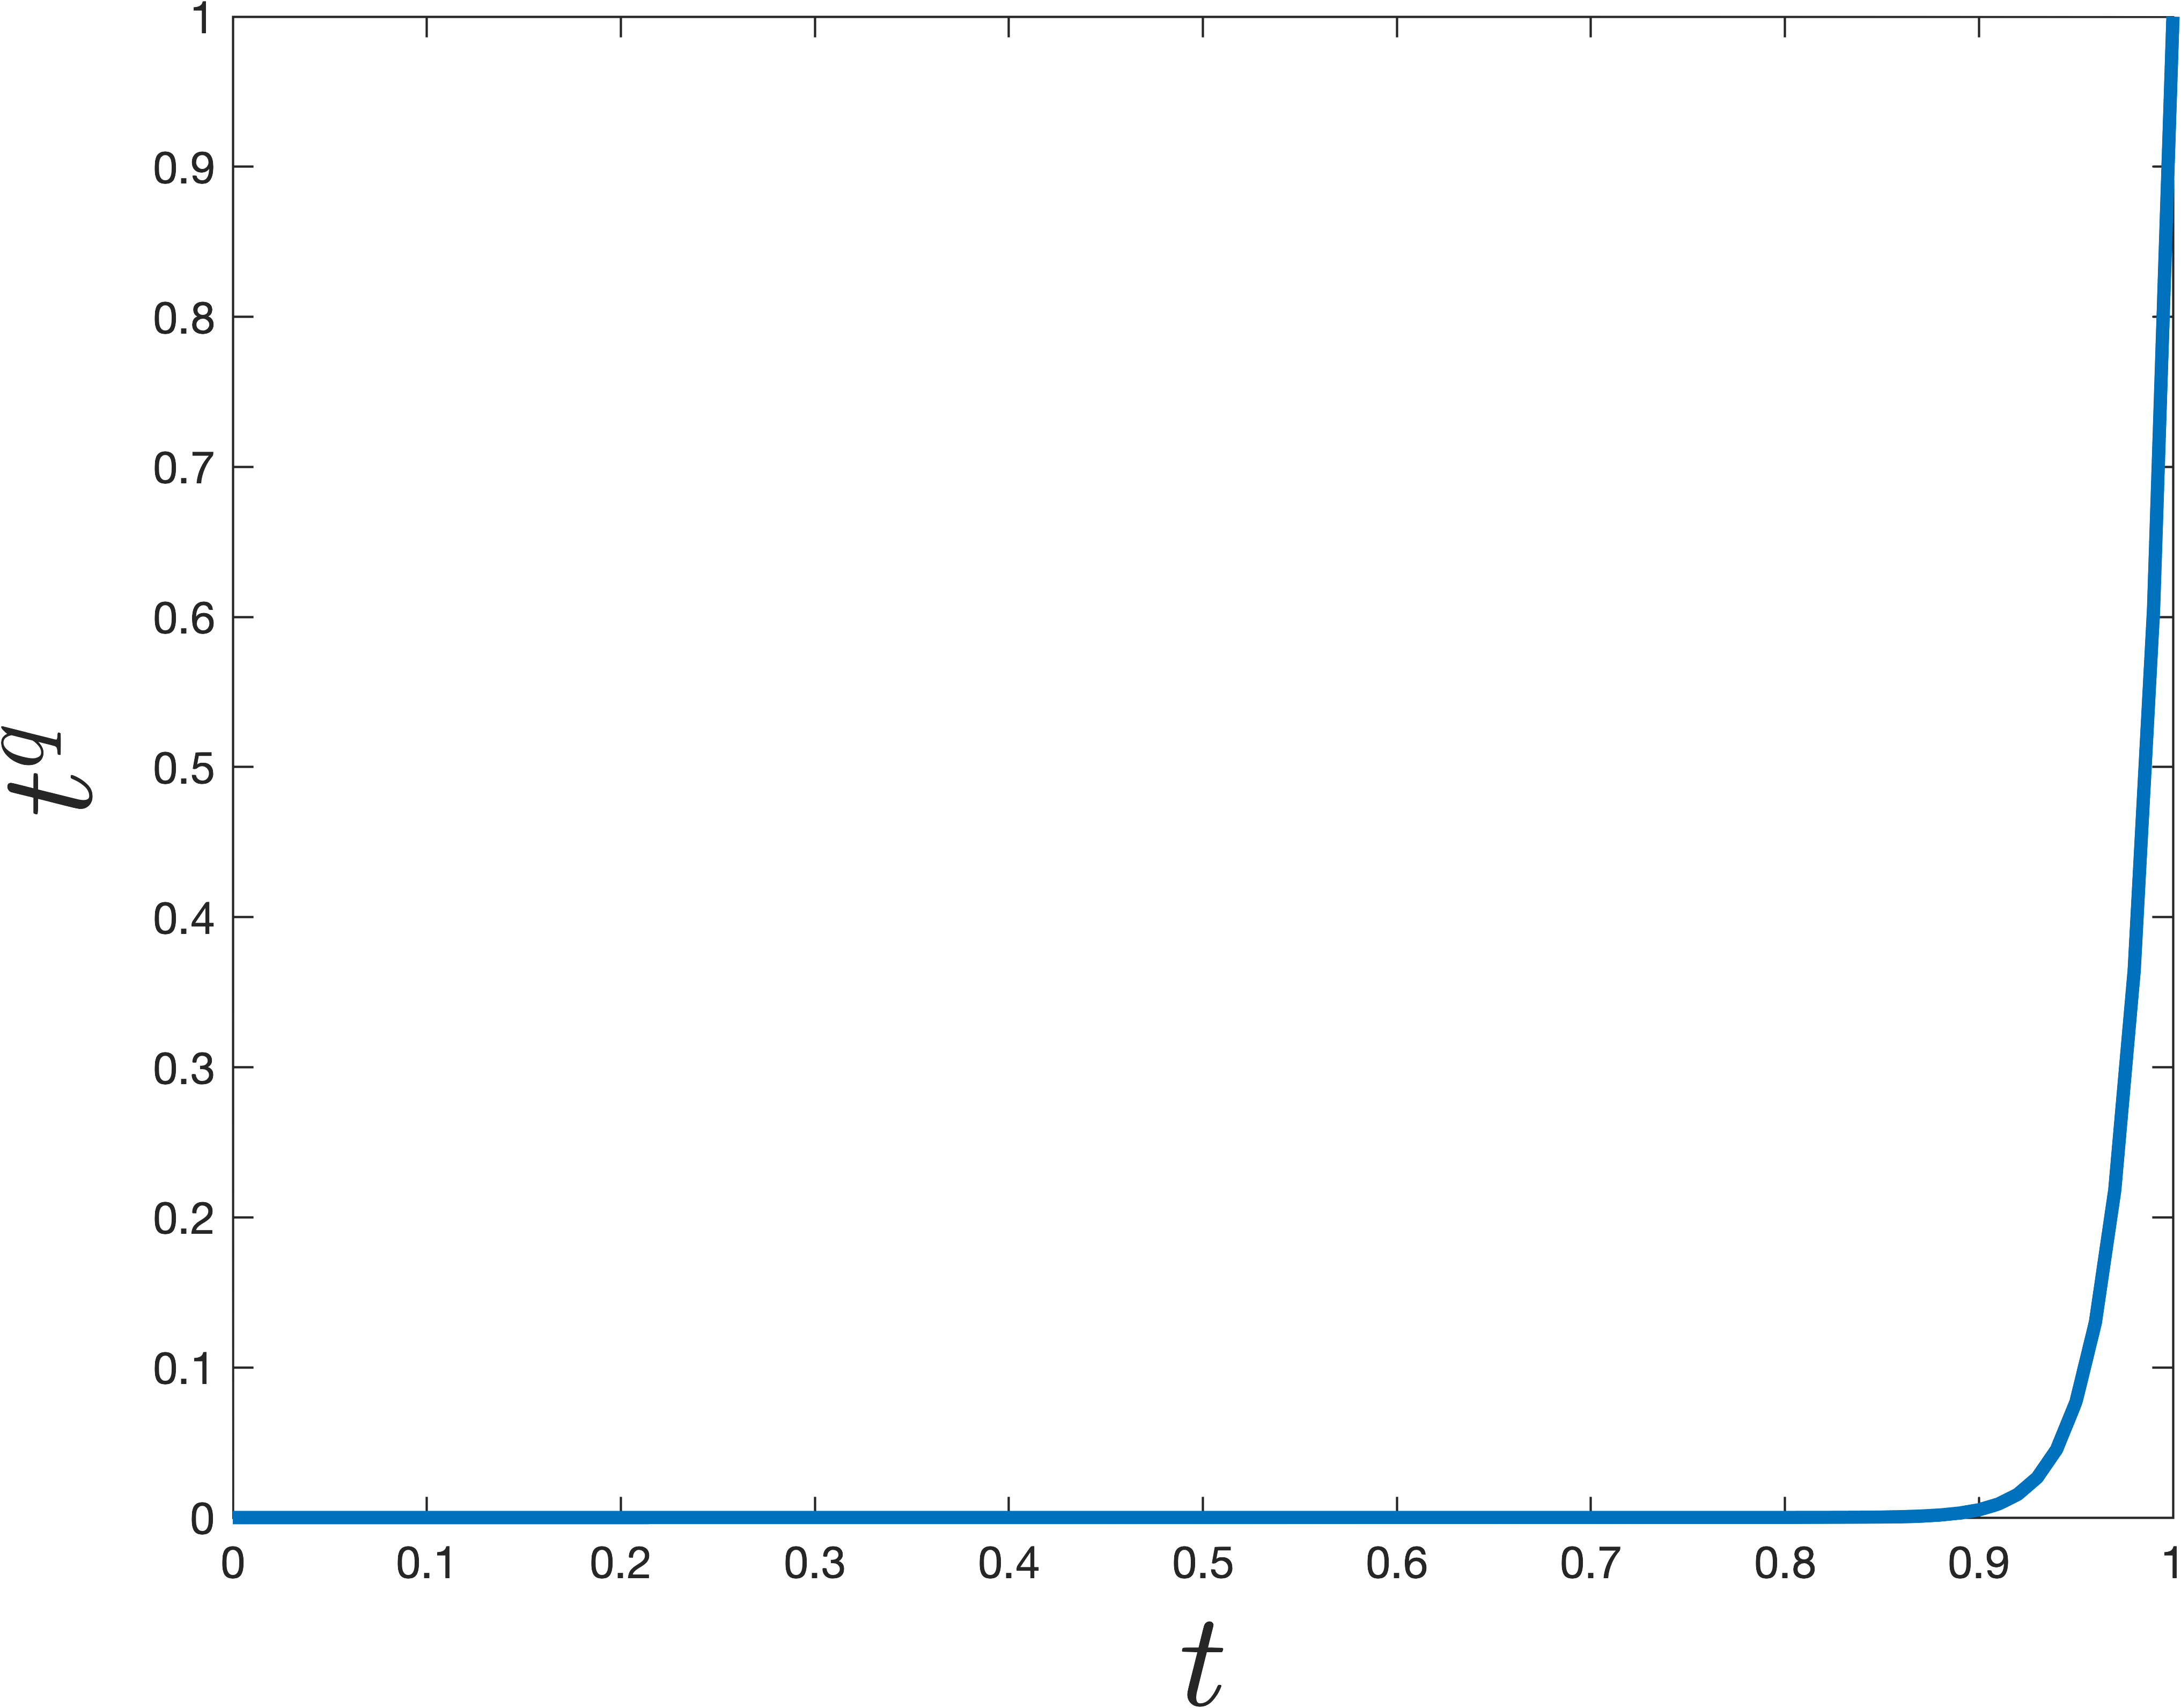
\includegraphics[width=.4\textwidth]{basic_jump.png} 
	\end{center}
	
	$\|\bv{X} - \bv{X}\bv{v}_{{p}^*}\bv{v}_{{p}^*}^T\|_F^2 \leq \|\bv{X} - \bv{X}\bv{v}_{\hat{p}}\bv{v}_{\hat{p}}^T\|_F^2 \approx \|\bv{X} - \bv{X}\bv{v}_{x^q}\bv{v}_{x^q}^T\|_F^2 \approx \|\bv{X} - \bv{X}\bv{v}_1\bv{v}_1^{T}\|_F^2$
	
	\textbf{\alert{Runtime}:} $O\left(\frac{\log(d/\epsilon)}{\sqrt{\epsilon}} \cdot \nnz(\bv{X})\right)$ vs. $O\left({\frac{\log(d/\epsilon)}{\epsilon}} \cdot \nnz(\bv{X})\right)$ 
\end{frame}


\begin{frame}[t]
	\frametitle{generalizations to larger $k$}
	\begin{itemize}
		\item Block Krylov methods
	\end{itemize}
	
	\begin{itemize}
		\item Let $\bv{G}\in \R^{d\times k}$ be a random Gaussian matrix.
		\item  $\mathcal{K}_q = \left[\bv{G}, \left(\bv{X}^T\bv{X}\right) \cdot \bv{G}, \left(\bv{X}^T\bv{X}\right)^2 \cdot \bv{G}, \ldots, \left(\bv{X}^T\bv{X}\right)^q \cdot \bv{G}\right]$
	\end{itemize}
	
	\begin{center}
		\alert{\textbf{Runtime}:} $O\left(\nnz(\bv{X}) \cdot k \cdot \frac{\log d/\epsilon}{\sqrt{\epsilon}}\right)$ to obtain a nearly optimal low-rank approximation.
	\end{center}
\end{frame}

\begin{frame}[standout]
	\begin{center}
			\large break
		\end{center}
\end{frame}

\begin{frame}
	\frametitle{spectral graph theory}
	\textbf{Main idea:} Understand \emph{graph data} by constructing natural matrix representations, and studying that matrix's \emph{spectrum} (eigenvalues/eigenvectors).
	\begin{center}
		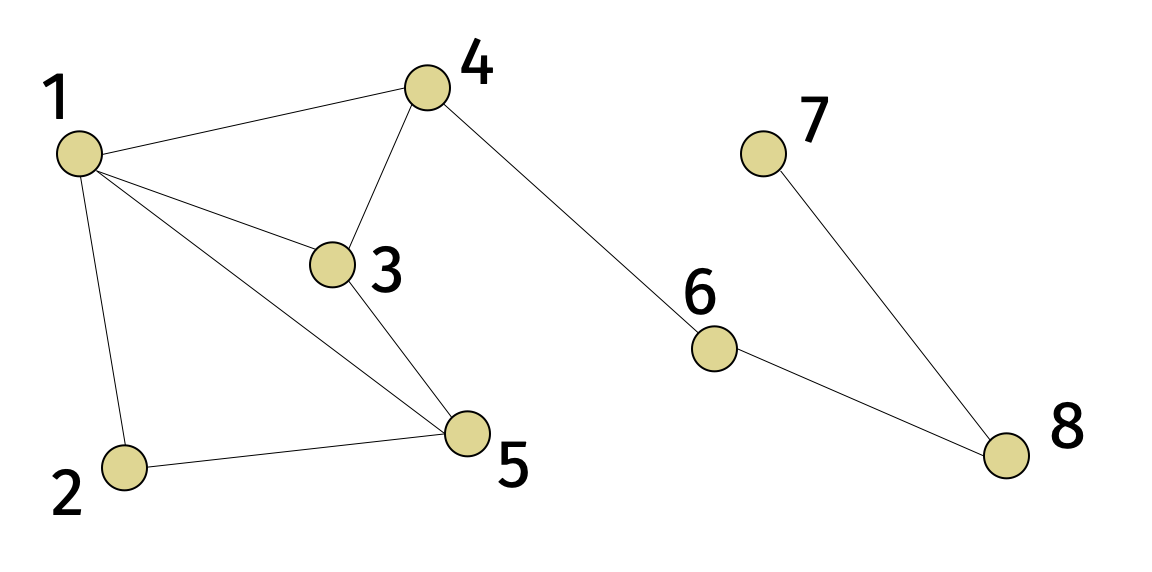
\includegraphics[width=.8\textwidth]{undirected_graph.png}
		
		For now assume $G = (V,E)$ is an undirected, unweighted graph with $n$ nodes.
	\end{center}
\end{frame}

\begin{frame}
	\frametitle{matrix representations of graphs}
	Two most common representations: $n\times n$ \emph{adjacency matrix} $\bv{A}$ and \emph{graph Laplacian} $\bv{L} = \bv{D}- \bv{A}$ where $\bv{D}$ is the diagonal degree matrix.
	\begin{center}
		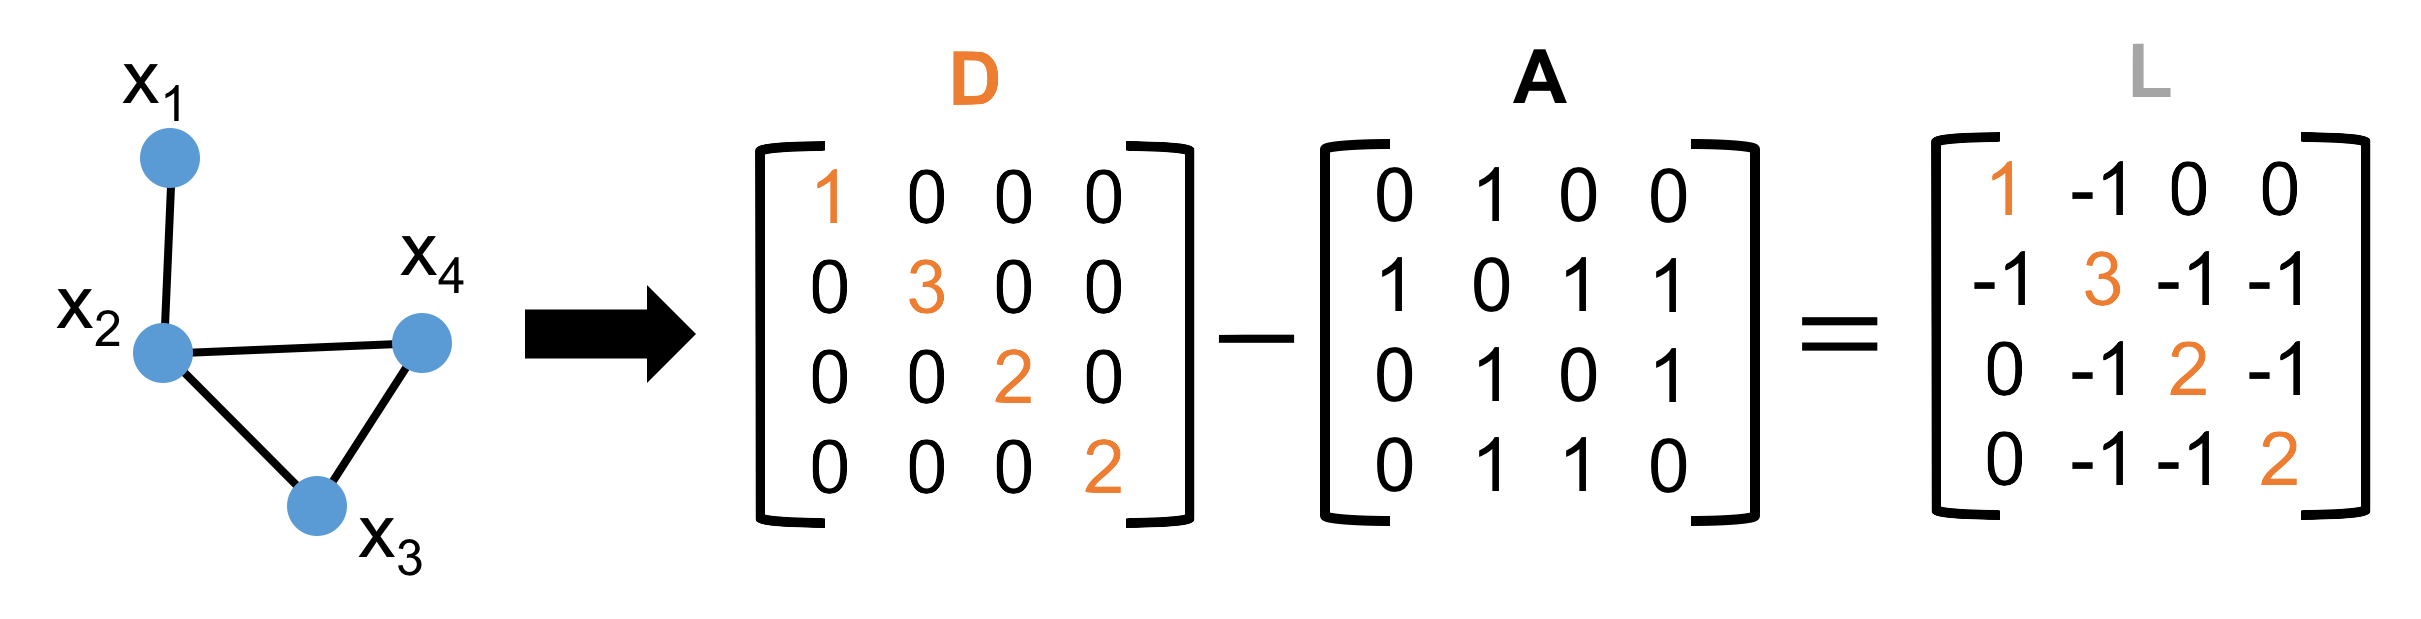
\includegraphics[width=\textwidth]{laplace.png}
	\end{center}

	Also common to look at normalized versions of both of these: $\bar{\bv{A}} = \bv{D}^{-1/2}\bv{A}\bv{D}^{-1/2}$ and $\bar{\bv{L}} = \bv{I} - \bv{D}^{-1/2}\bv{A}\bv{D}^{-1/2}$. 
\end{frame}

\begin{frame}
	\frametitle{spectral graph theory tidbits}
	\begin{itemize}
		\item If $\bv{L}$ have $k$ eigenvalues equal to $0$, then $G$ has $k$ connected components. 
		\item Sum of cubes of $\bv{A}$'s eigenvalues is equal to number of triangles in the graph times $6$. 
		\item Sum of eigenvalues to the power $q$ is proportional to the number of $q$ cycles. 
		\item \alert{Today: Eigenvectors of super useful in clustering graph data.}
	\end{itemize}
\end{frame}


\begin{frame}[t]
	\frametitle{matrix representations of graphs}
		\frametitle{the laplacian view}
		\begin{center}
			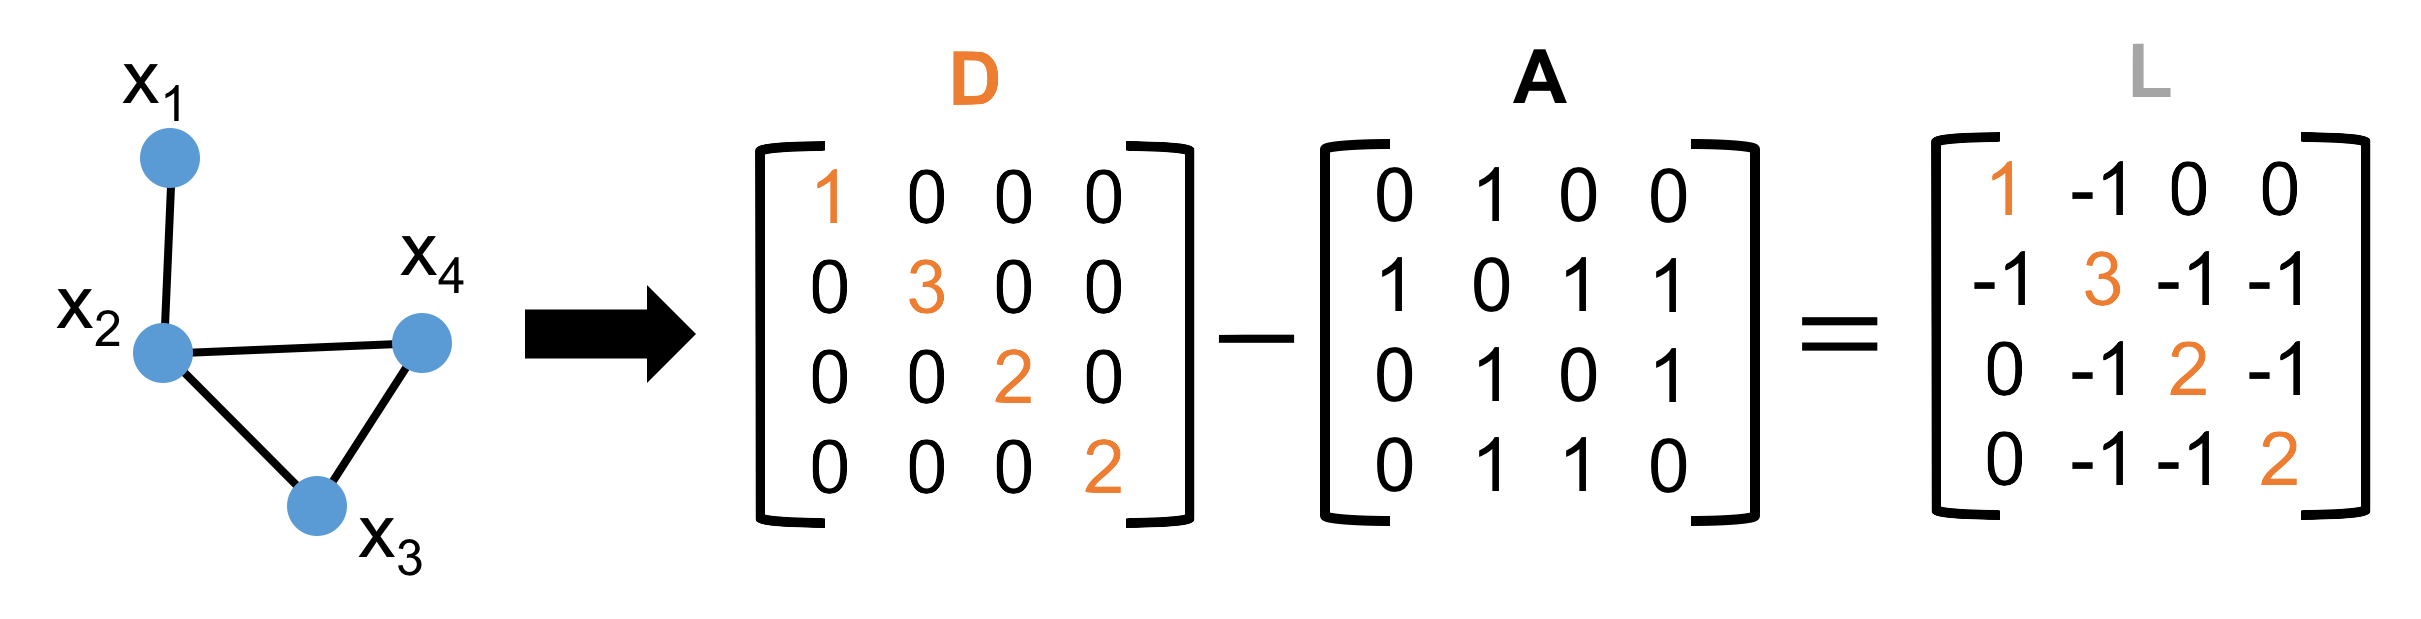
\includegraphics[width=.95\textwidth]{laplace.png}
			
			$\bv{L} = \bv{B}^T\bv{B}$ where $B$ is the signed ``edge-vertex incidence'' matrix.
		\end{center}
		$\bv{B} = $	
\end{frame}

\begin{frame}[t]
	\frametitle{matrix representations of graphs}
	\frametitle{the laplacian view}
	\begin{align*}
		\bv{L} = \bv{B}^T\bv{B} = \bv{b}_1\bv{b}_1^T + \bv{b}_2\bv{b}_2^T + \ldots + \bv{b}_m\bv{b}_m^T,
	\end{align*}
where $\bv{b}_i$ is the $i^\text{th}$ row of $\bv{B}$ (each row corresponds to a single edge). 
	\begin{center}
	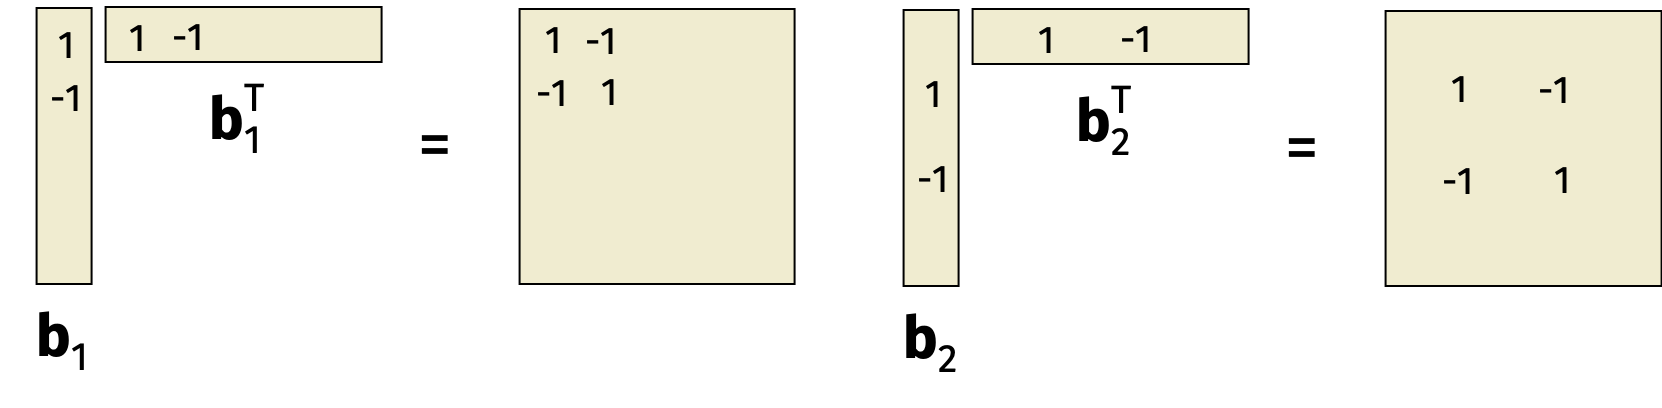
\includegraphics[width=\textwidth]{edge_vertex.png}
\end{center}
\end{frame}

\begin{frame}[t]
	\frametitle{the laplacian view}
	\textbf{Conclusions from $\bv{L} = \bv{B}^T\bv{B}$}
	\begin{itemize}
		\item $\bv{L}$ is positive semidefinite: $\bv{x}^T\bv{L}\bv{x} \geq 0$ \emph{for all} $\bv{x}$. 
		\vspace{1em}
		\item $\bv{L} = \bv{V}\bs{\Sigma}^2\bv{V}^T$ where $\bv{U}\bs{\Sigma}\bv{V}^T$ is $\bv{B}$'s SVD. Columns of $\bv{V}$ are \emph{eigenvectors} of $\bv{L}$.
		\vspace{1em}
		\item 	\alert{For any vector $\bv{x}\in \R^n$, 
		\begin{align*}
			\bv{x}^T L \bv{x} = \sum_{(i,j)  \in E} (\bv{x}(i)- \bv{x}(j))^2. 
		\end{align*}}
	\end{itemize}	
\end{frame}

\begin{frame}[t]
	\frametitle{the laplacian view}
	$\bv{x}^T L \bv{x} = \sum_{(i,j)  \in E} (\bv{x}(i)- \bv{x}(j))^2$. So $\bv{x}^T L \bv{x}$ is small if $\bv{x}$ is a ``smooth'' function with respect to the graph. 
	\begin{center}
		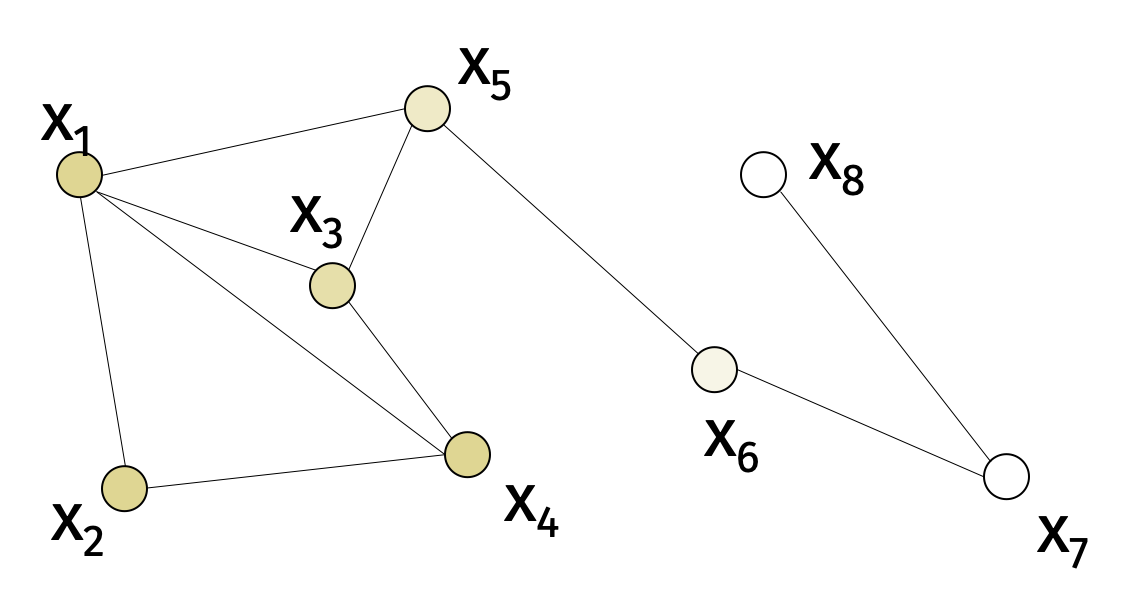
\includegraphics[width=.8\textwidth]{smooth_func.png}
		
		Eigenvectors of the Laplacian with \emph{small eigenvalues} correspond to \emph{smooth functions} over the graph.
	\end{center}
\end{frame}

\begin{frame}[t]
	\frametitle{another example of a smooth function}
	Any function that only has a large change across a small cut in the graph is also smooth. 
	\begin{center}
		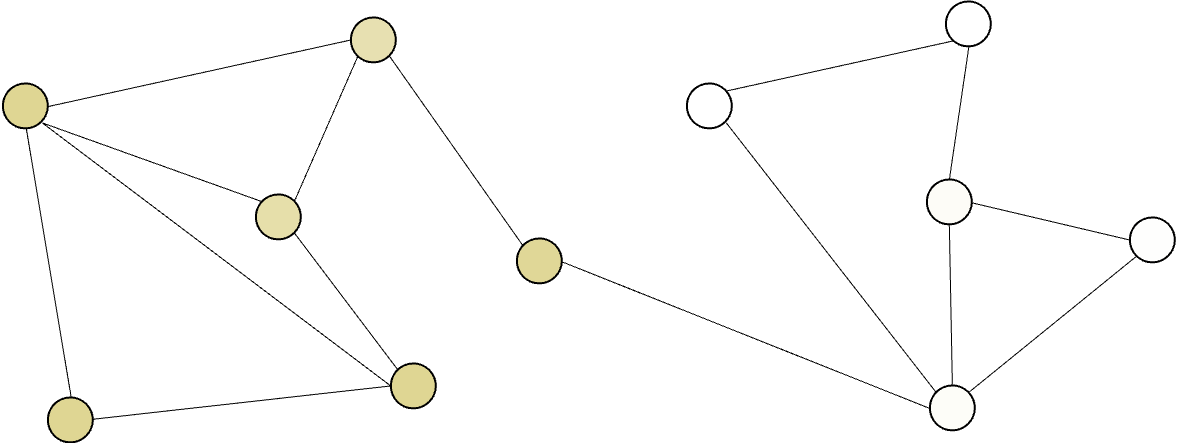
\includegraphics[width=.8\textwidth]{smooth_func2.png}
	\end{center}
\end{frame}

\begin{frame}
	\frametitle{smallest laplacian eigenvector}
	\begin{center}
		\textbf{Courant–Fischer min-max principle}
	\end{center}
	Let $\bv{V} = [\bv{v}_1,\ldots,\bv{v}_n]$ be the eigenvectors of $\bv{L}$.
	
	\begin{align*}
		\bv{v}_n &= \argmin_{\|\bv{v}\|=1} \bv{v}^T\bv{L}\bv{v} \\
		\bv{v}_{n-1} &= \argmin_{\|\bv{v}\|=1,\bv{v} \perp \bv{v}_n} \bv{v}^T\bv{L}\bv{v} \\
		\bv{v}_{n-2}  &= \argmin_{\|\bv{v}\|=1,\bv{v} \perp \bv{v}_n,\bv{v}_{n-1}} \bv{v}^T\bv{L}\bv{v} \\
		&\vdots \\
		\bv{v}_1 &= \argmin_{\|\bv{v}\|=1,\bv{v} \perp \bv{v}_n,\ldots,\bv{v}_2} \bv{v}^T\bv{L}\bv{v} 
	\end{align*}
\end{frame}

\begin{frame}
	\frametitle{largest laplacian eigenvector}
	\begin{center}
		\textbf{Courant–Fischer min-max principle}
	\end{center}
	Let $\bv{V} = [\bv{v}_1,\ldots,\bv{v}_n]$ be the eigenvectors of $\bv{L}$.
	
	\begin{align*}
		\bv{v}_1 &= \argmax_{\|\bv{v}\|=1} \bv{v}^T\bv{L}\bv{v} \\
		\bv{v}_2 &= \argmax_{\|\bv{v}\|=1,\bv{v} \perp \bv{v}_1} \bv{v}^T\bv{L}\bv{v} \\
		\bv{v}_3 &= \argmax_{\|\bv{v}\|=1,\bv{v} \perp \bv{v}_1,\bv{v}_2} \bv{v}^T\bv{L}\bv{v} \\
		&\vdots \\
		\bv{v}_n &= \argmax_{\|\bv{v}\|=1,\bv{v} \perp \bv{v}_1,\ldots,\bv{v}_{n-1}} \bv{v}^T\bv{L}\bv{v} 
	\end{align*}
\end{frame}

\begin{frame}
	\frametitle{example application of spectral graph theory}
	\begin{itemize}
		\item Study \emph{graph partitioning} problem important in 1) understanding social networks 2) nonlinear clustering in unsupervised machine learning (spectral clustering).  3) Graph visualization 4) Mesh partitioning
		\item See how this problem can be solved heuristically using Laplacian eigenvectors. 
		\item Give a full analysis of the method for a common \emph{random graph model}.
		\item Use two tools: \emph{matrix concentration} and \emph{eigenvector perturbation bounds}.
	\end{itemize}
\end{frame}


\begin{frame}
	\frametitle{balanced cut}
	\textbf{Common goal:} Given a graph $G = (V,E)$, partition nodes along a cut that:
	\begin{itemize}
		\item Has few crossing edges: $|\{(u,v) \in E: u\in S,v\in T \}|$ is small.
		\item Separates large partitions: $|S|,|T|$ are not too small.
	\end{itemize}
\vspace{-.5em}
	\begin{center}
		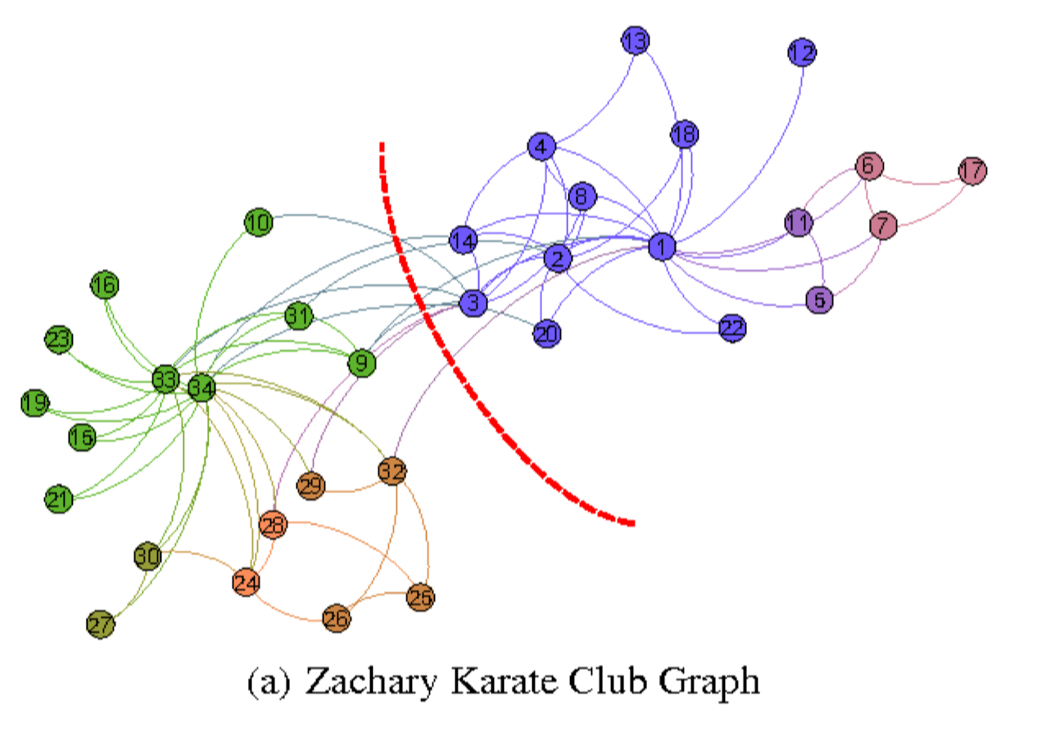
\includegraphics[width=.55\textwidth]{karate.png}
		\vspace{-1em}
	\end{center}
	Important in understanding \emph{community structure} in social networks. 
\end{frame}

\begin{frame}
	\frametitle{social networks in the 1970s}
	\begin{center}
	Wayne W. Zachary (1977). An Information Flow Model for Conflict and Fission in Small Groups.
	\end{center}
	
	\small{
	``The network captures 34 members of a karate club, documenting links between pairs of members who interacted outside the club. During the study a conflict arose between the administrator "John A" and instructor "Mr. Hi" (pseudonyms), which led to the split of the club into two. Half of the members formed a new club around Mr. Hi; members from the other part found a new instructor or gave up karate. Based on collected data Zachary correctly assigned all but one member of the club to the groups they actually joined after the split.'' -- Wikipedia
}
	
	\begin{center}
		\normalsize{\textbf{Beautiful paper -- definitely worth checking out!}}
	\end{center}
\end{frame}


\begin{frame}
	\frametitle{balanced cut}
	\textbf{Common goal:} Given a graph $G = (V,E)$, partition nodes along a cut that:
	\begin{itemize}
		\item Has few crossing edges: $|\{(u,v) \in E: u\in S,v\in T \}|$ is small.
		\item Separates large partitions: $|S|,|T|$ are not too small.
	\end{itemize}
	\vspace{-.5em}
	\begin{center}
		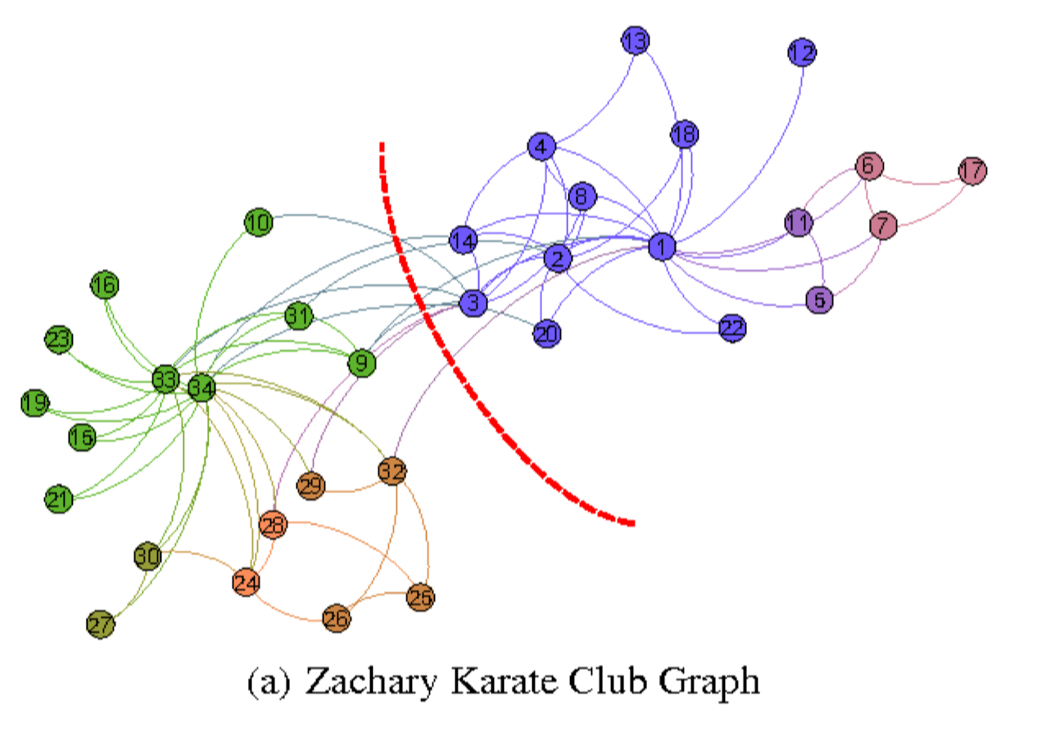
\includegraphics[width=.55\textwidth]{karate.png}
		\vspace{-1em}
	\end{center}
	Important in understanding \emph{community structure} in social networks. 
\end{frame}



\begin{frame}
	\frametitle{spectral clustering}
	\textbf{Idea:} Construct synthetic graph for data that is hard to cluster.
	
	\begin{center}
		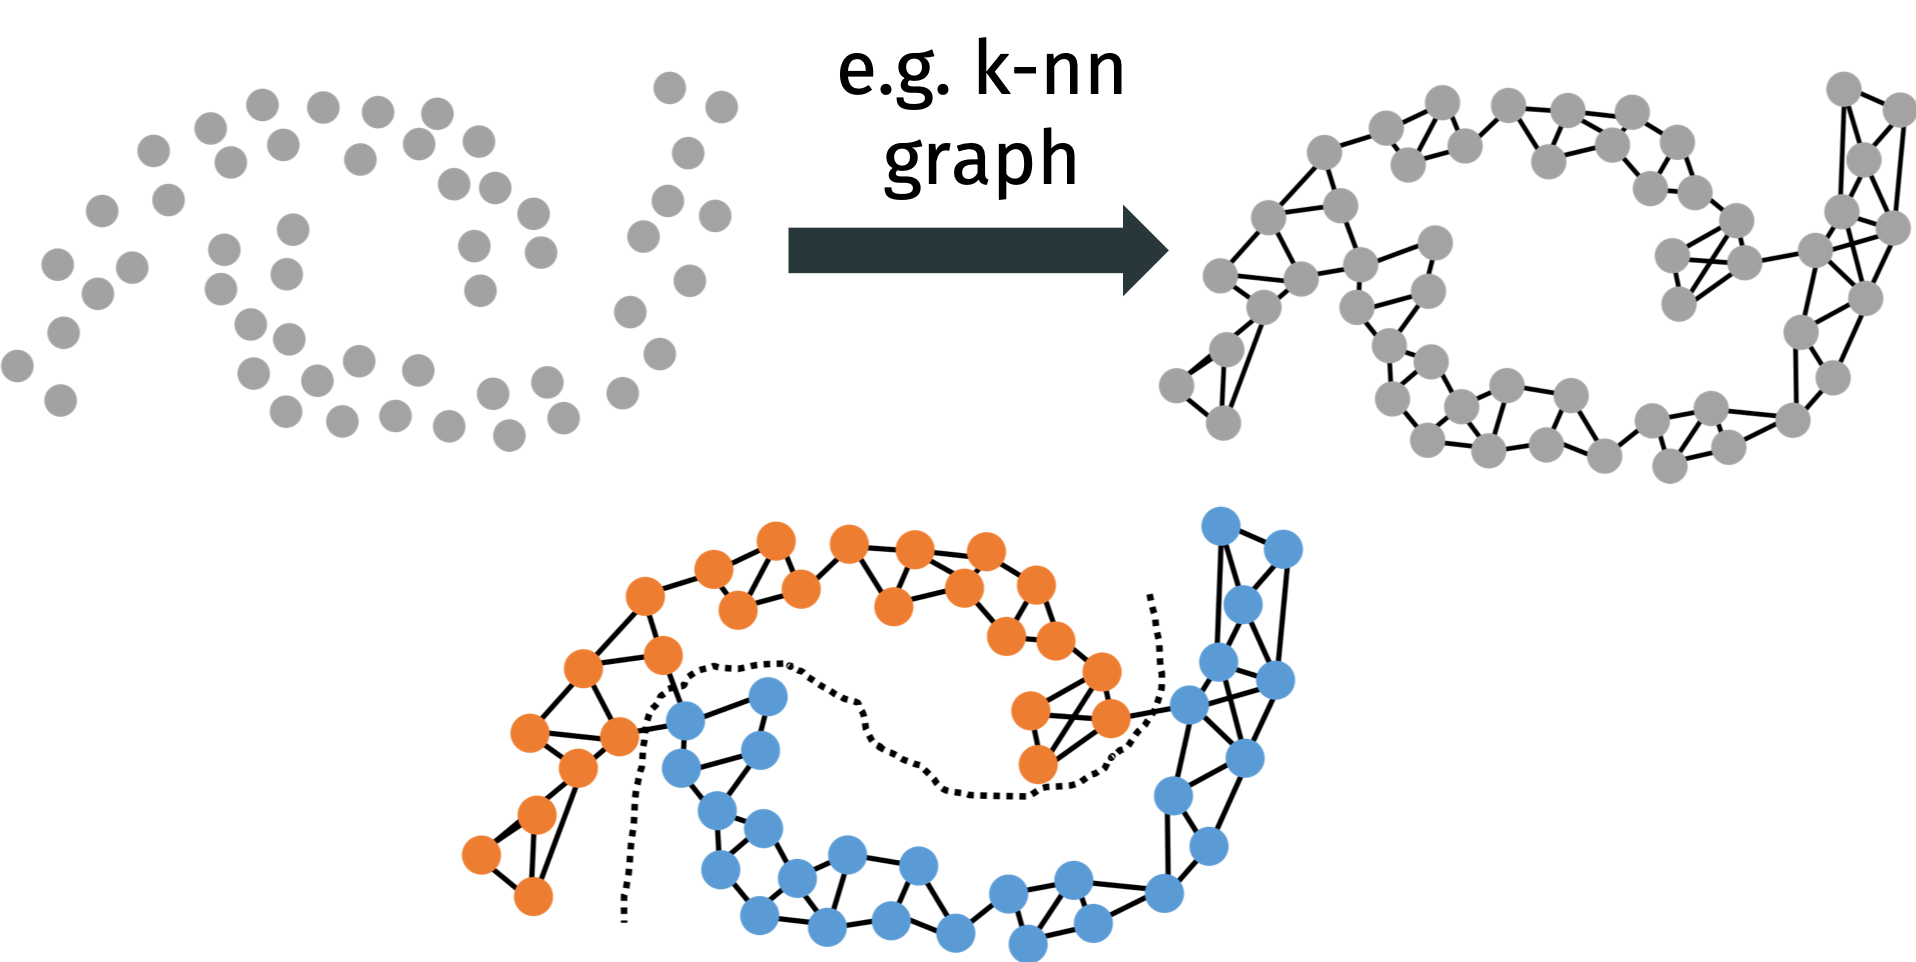
\includegraphics[width=\textwidth]{cut_clustering.png}
		
		Spectral Clustering, Laplacian Eigenmaps, Locally linear embedding, Isomap, etc.
	\end{center}
	
\end{frame}

\begin{frame}[t]
	\frametitle{spectral graph partitioning}
	There are many way's to formalize Zachary's problem:
	
		\textbf{$\beta$-Balanced Cut:}
	\begin{align*}
		&\min_{S} {\cut(S, V\setminus S)} & &\text{such that} & &\min\left(|S|,|V\setminus S|\right) \geq \beta \text{ for } \beta \leq .5
	\end{align*}
	
	\textbf{Sparsest Cut:}
	\begin{align*}
		\min_{S} \frac{\cut(S, V\setminus S)}{\min\left(|S|,|V\setminus S|\right)}
	\end{align*}



	Most formalizations lead to NP-hard problems. Lots of interest in designing polynomial time approximation algorithms, but tend to be slow. In practice, much simpler methods based on the \emph{graph spectrum} are used. 
	
	\begin{center}
		\textbf{Spectral  methods run in at worst $O(n^3)$ time (faster if you use iterative methods).}
	\end{center}
\end{frame}

\begin{frame}
		\frametitle{spectral graph partitioning}
	\textbf{Basic spectral clustering method:}
	\begin{itemize}
		\item Compute \emph{second} smallest eigenvalue of graph, $\bv{v}_{n-1}$.
		\item $\bv{v}_{n-1}$ has an entry for every node $i$ in the graph.
		\item If the $i^{\text{th}}$ entry is positive, put node $i$ in $T$.
		\item Otherwise if the $i^{\text{th}}$ entry is negative, put $i$ in $S$.
	\end{itemize}	
\begin{center}
	\textbf{\alert{This shouldn't make much sense yet!} We will see that is a ``relax and round'' algorithm in disguise.}
\end{center}
\end{frame}


\begin{frame}[t]
	\frametitle{the laplacian view}
	\textbf{Another conclusion from $\bv{L} = \bv{B}^T\bv{B}$}:
	
	
	For a \emph{cut indicator vector} $\bv{c} \in \{-1,1\}^n$ with $\bv{c}(i) = -1$ for $i \in S$ and $\bv{c}(i) = 1$ for $i \in T = V \setminus S$:
		\begin{align}
			 \bv{c}^T L \bv{c} = \sum_{(i,j)  \in E} (\bv{c}(i)- \bv{c}(j))^2 = 4 \cdot \cut(S,T).
		\end{align}
	
	\begin{center}
		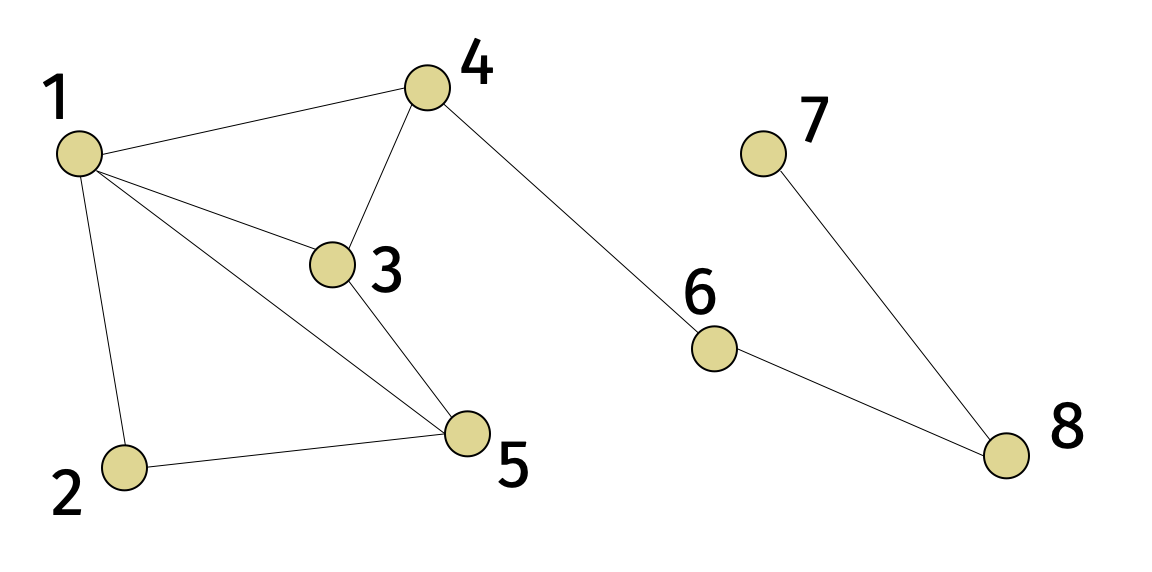
\includegraphics[width=.8\textwidth]{undirected_graph.png}
	\end{center}
\end{frame}

\begin{frame}
	\frametitle{the laplacian view}
	\begin{center}
	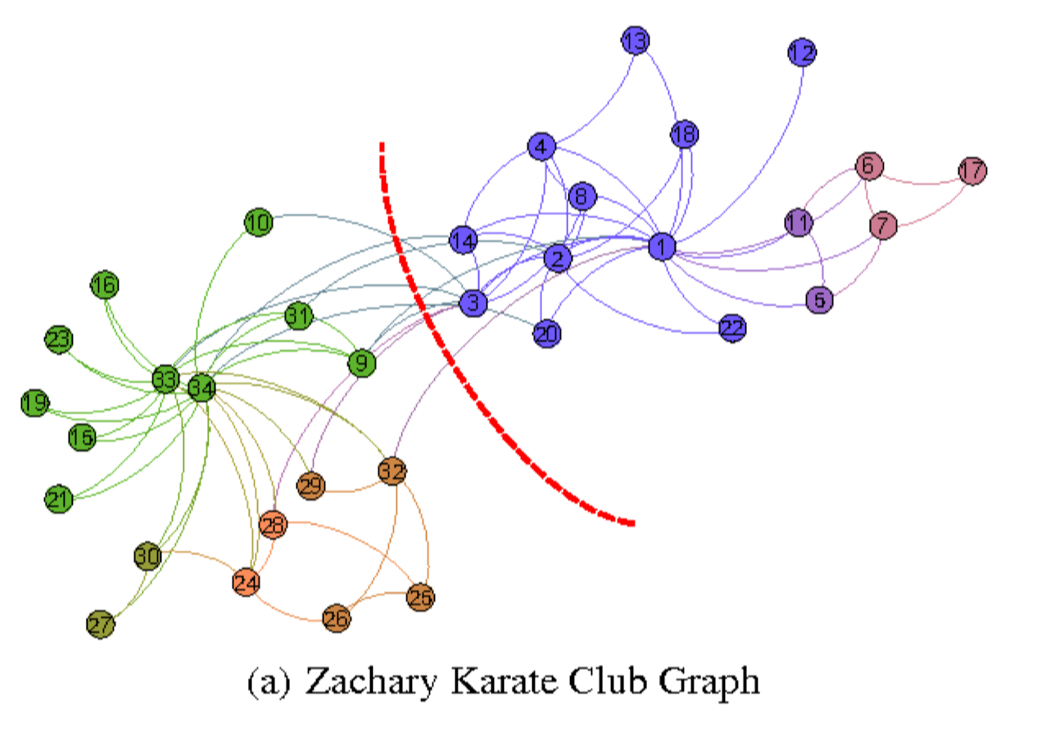
\includegraphics[width=.4\textwidth]{karate.png}
	\end{center}
	For a \emph{cut indicator vector} $\bv{c} \in \{-1,1\}^n$ with $\bv{c}(i) = -1$ for $i \in S$ and $\bv{c}(i) = 1$ for $i \in T$:
	\begin{itemize}
		\item $\bv{c}^T L \bv{c} = 4 \cdot cut(S,T)$.
		\item $\bv{c}^T \bv{1} = |T| - |S|$.
	\end{itemize}
	Want to minimize both $\bv{c}^T L \bv{c}$ (cut size) and $|\bv{c}^T \bv{1}|$ (imbalance).
\end{frame}

\begin{frame}
	\frametitle{the laplacian view}
	\begin{center}
		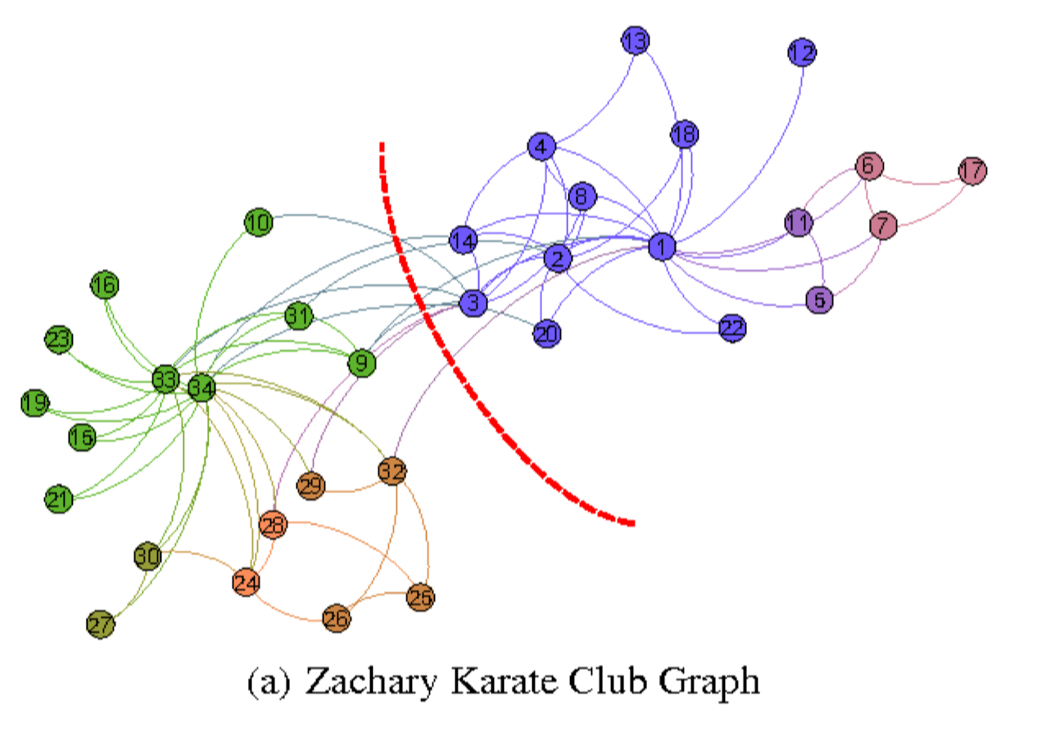
\includegraphics[width=.4\textwidth]{karate.png}
	\end{center}
	Equivalent formulation if we divide everything by $\sqrt{n}$ so that $\bv{c}$ has norm $1$. Then $\bv{c} \in \{-\frac{1}{\sqrt{n}},\frac{1}{\sqrt{n}}\}^n$ and:
	\begin{itemize}
		\item $\bv{c}^T L \bv{c} = \frac{4}{n} \cdot cut(S,T)$.
		\item $\bv{c}^T \bv{1} = \frac{1}{\sqrt{n}}(|T| - |S|)$.
	\end{itemize}
	Want to minimize both $\bv{c}^T L \bv{c}$ (cut size) and $|\bv{c}^T \bv{1}|$ (imbalance).
\end{frame}

\begin{frame}
	\frametitle{relax and round}
	Consider the ``perfectly balanced'' version of the balanced cut problem:
	\begin{align*}
		\min_{\bv{c} \in \{-\frac{1}{\sqrt{n}},\frac{1}{\sqrt{n}}\}^n} \bv{c}^T\bv{L}\bv{c} \text{ such that } \bv{c}^T\bv{1} = 0.
	\end{align*}
	\textbf{Claim:} If we \emph{relax} the constraint $\bv{c} \in \{-\frac{1}{\sqrt{n}}\frac{1}{\sqrt{n}}\}^n$ to $\|\bv{c}\|_2 = 1$, then this problem is exactly minimized by the second smallest eigenvector $\bv{v}_{n-1}$ of $\bv{L}$. 

	\textbf{Approach:} Relax, find $\bv{v}_{n-1}$, then round back to a vector with $-\frac{1}{\sqrt{n}},\frac{1}{\sqrt{n}}$ entries.
\end{frame}




\begin{frame}[t]
	\frametitle{smallest laplacian eigenvector}
	The smallest eigenvector/singular vector $\bv{v}_n$ satisfies:
	\begin{align*}
	\bv{v}_n = \frac{1}{\sqrt{n}} \cdot \bv{1} = \argmin_{v \in \R^n\text{ with } \norm{\bv{v}} = 1} \bv{v}^T L \bv{v}
	\end{align*}
	with $\bv{v}_n^T  L \bv{v}_n = 0$. 
	
	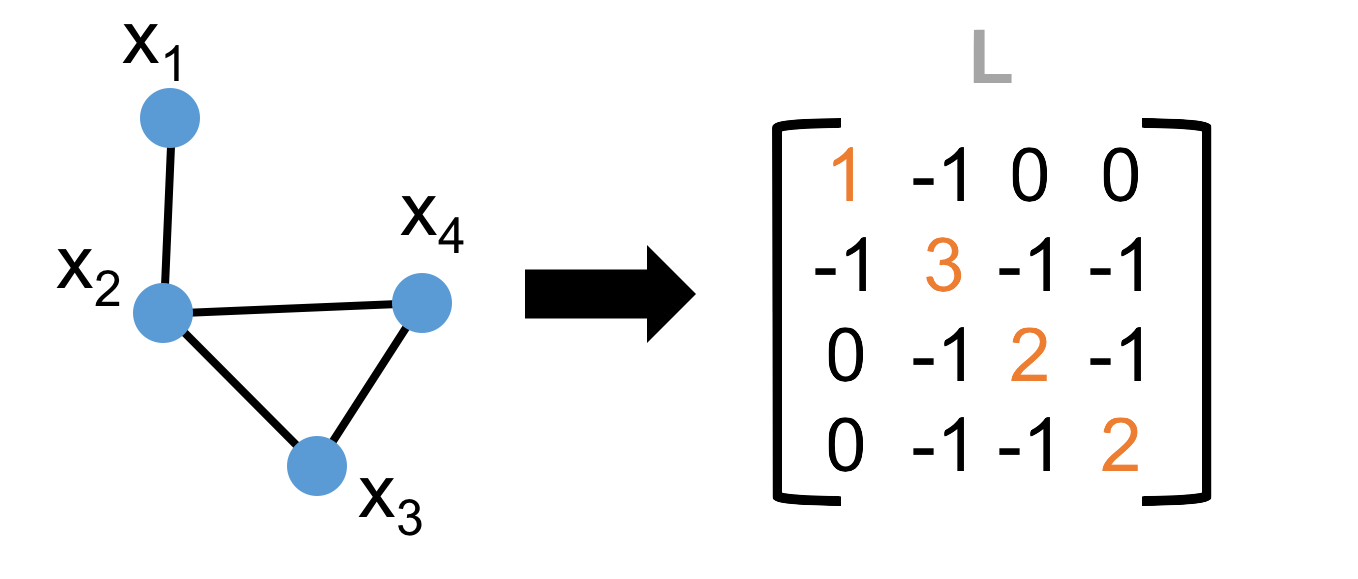
\includegraphics[width=.5\textwidth]{laplace_compact.png}
\end{frame}

\begin{frame}
	\frametitle{second smallest laplacian eigenvector}
	By Courant-Fischer, $\bv{v}_{n-1}$ is given by:
	\begin{align*}
	\bv{v}_{n-1} = \argmin_{\norm{\bv{v}} = 1,\ {\bv{v}_n^T \bv{v} = 0}} \bv{v}^T L \bv{v}
	\end{align*}
	which is equivalent to
	\begin{align*}
		\bv{v}_{n-1} = \argmin_{\norm{\bv{v}} = 1,\ {\bv{1}^T \bv{v} = 0}} \bv{v}^T L \bv{v}.
	\end{align*}
\end{frame}

\begin{frame}
	\frametitle{cutting with the  second laplacian eigenvector}
	\textbf{Final relax and round algorithm:} Compute 
	$$\bv{v}_{n-1} = \argmin_{v \in \R^n \text{ with } \norm{\bv{v}} = 1,\ \alert{\bv{v}^T \bv{1} = 0}} \bv{v}^T L \bv{v}$$ Set $S$ to be all nodes with $\bv{v}_{n-1}(i) < 0$, and $T$ to be all with $\bv{v}_{n-1}(i) \ge 0$. I.e. set $\bv{c} = \sign(\bv{v}_{n-1})$
	\begin{center}
		\vspace{-1em}
		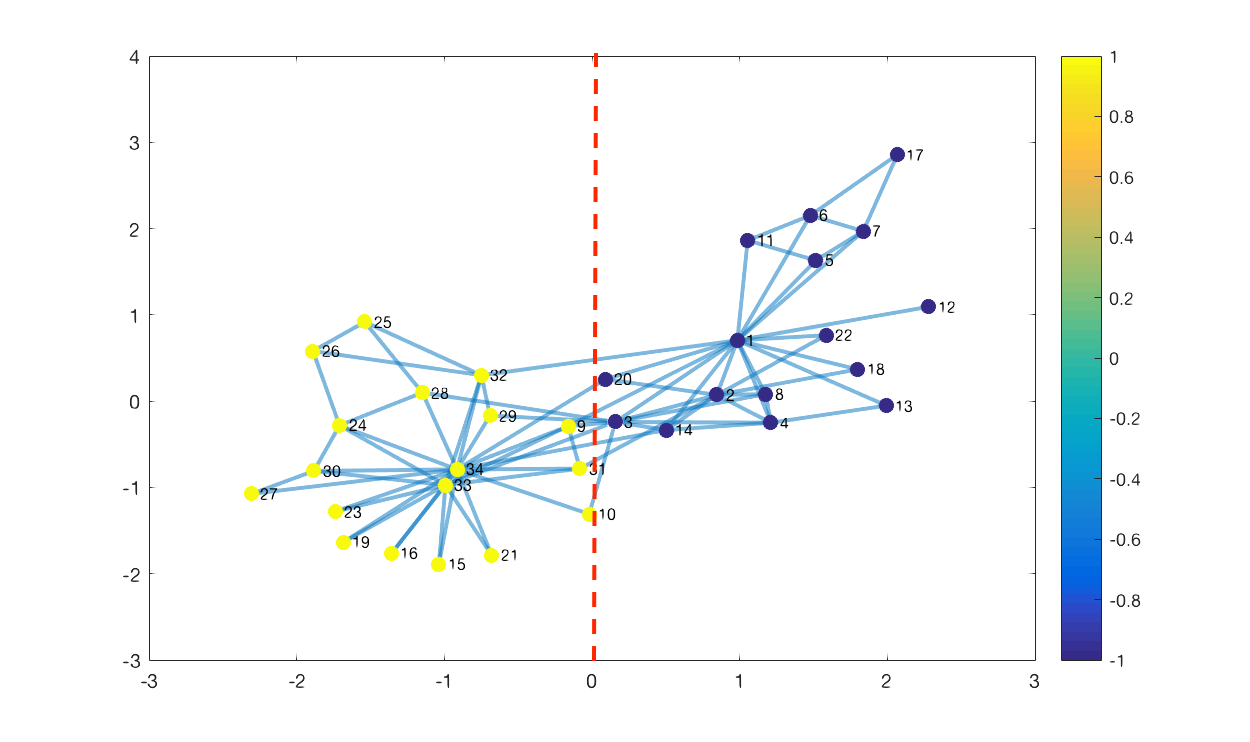
\includegraphics[width=.9\textwidth]{cut2-fix.png}
	\end{center}
\end{frame}

\begin{frame}
	\frametitle{spectral partitioning in practice}
	The Shi-Malik normalized cuts algorithm is one of the most commonly used variants of this approach, using the normalized Laplacian $\mathbf{\overline L} = \bv{D}^{-1/2} \bv{L} \bv{D}^{-1/2}$.
	
		\textbf{Important consideration:} What to do when we want to split the graph into more than two parts?
		\begin{center}
				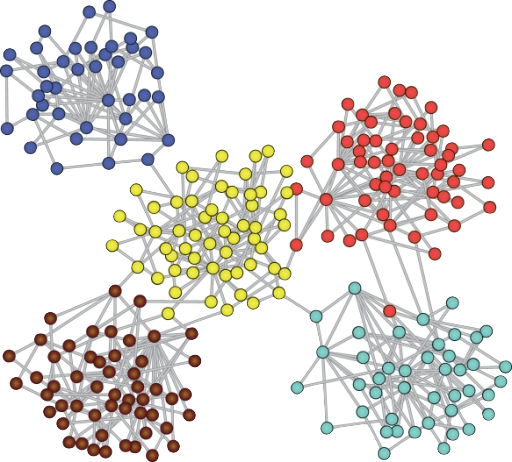
\includegraphics[width=.33\textwidth]{multiway.png}
		\end{center}
\end{frame}

\begin{frame}
	\frametitle{spectral partitioning in practice}
	\textbf{Spectral Clustering:}
	\begin{itemize}
		\item Compute smallest $k$ eigenvectors $\bv{v}_{n-1}, \ldots, \bv{v}_{n-\ell}$ of $\mathbf{L}$.
		\item Represent each node by its corresponding row in $\bv{V} \in \R^{n \times \ell}$ whose rows are  $\bv{v}_{n-1}, \ldots \bv{v}_{n-\ell}$.
		\item Cluster these rows using $k$-means clustering (or really any clustering method).
		\item Often we choose $\ell = k$, but not necessarily. 
	\end{itemize}
\end{frame}

\begin{frame}
	\frametitle{laplacian embedding}
	\begin{center}
		\textbf{Original Data:} (not linearly separable)
			
			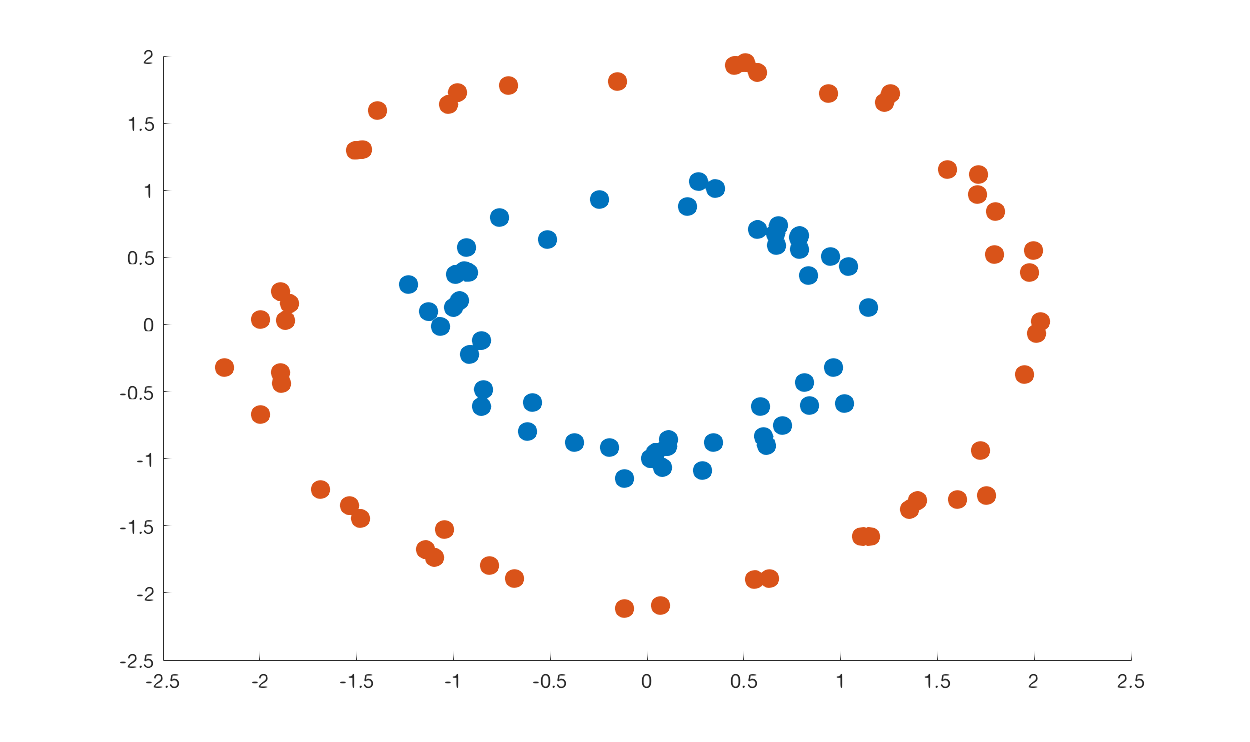
\includegraphics[width=.7\textwidth]{circ.png}
	\end{center}
\end{frame}

\begin{frame}
	\frametitle{laplacian embedding}
	\begin{center}
			\textbf{$k$-Nearest Neighbors Graph:}
			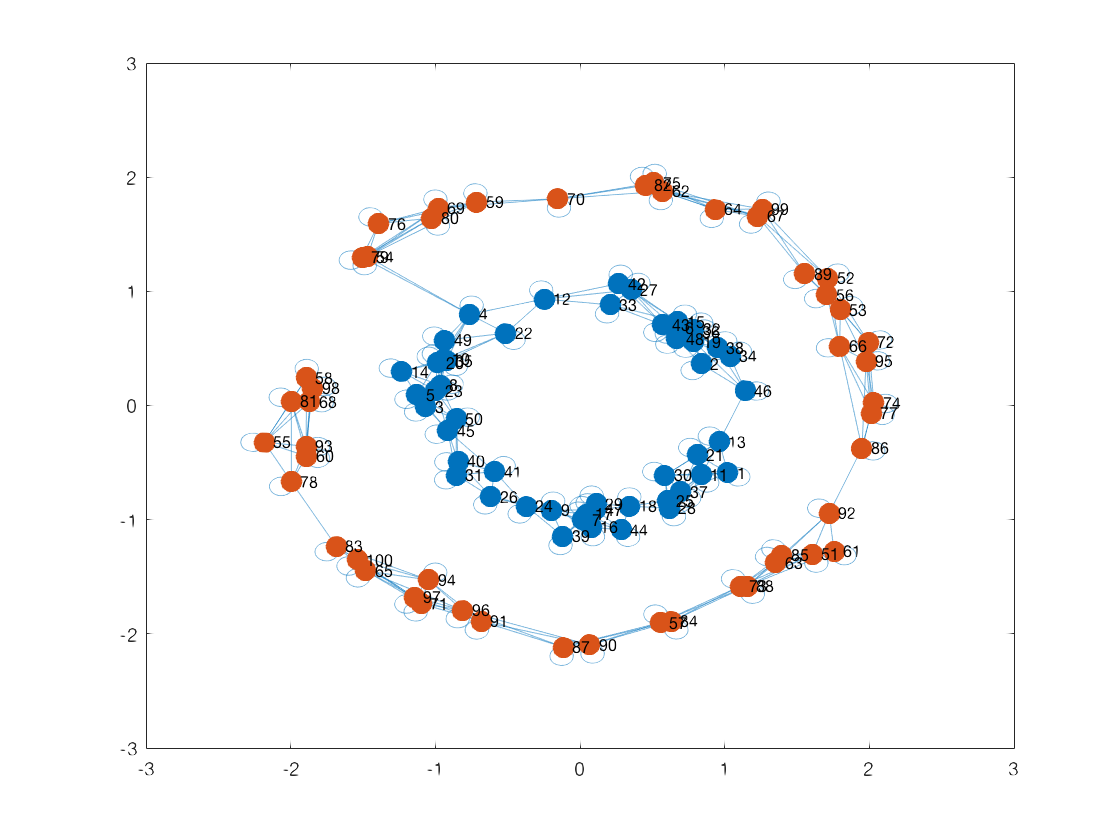
\includegraphics[width=.7\textwidth]{circ2.png}
	\end{center}
\end{frame}

\begin{frame}
	\frametitle{laplacian embedding}
	\begin{center}
	\textbf{Embedding with eigenvectors $\bv{v}_{n-1}, \bv{v}_{n-2}$:} (linearly separable) 
			
			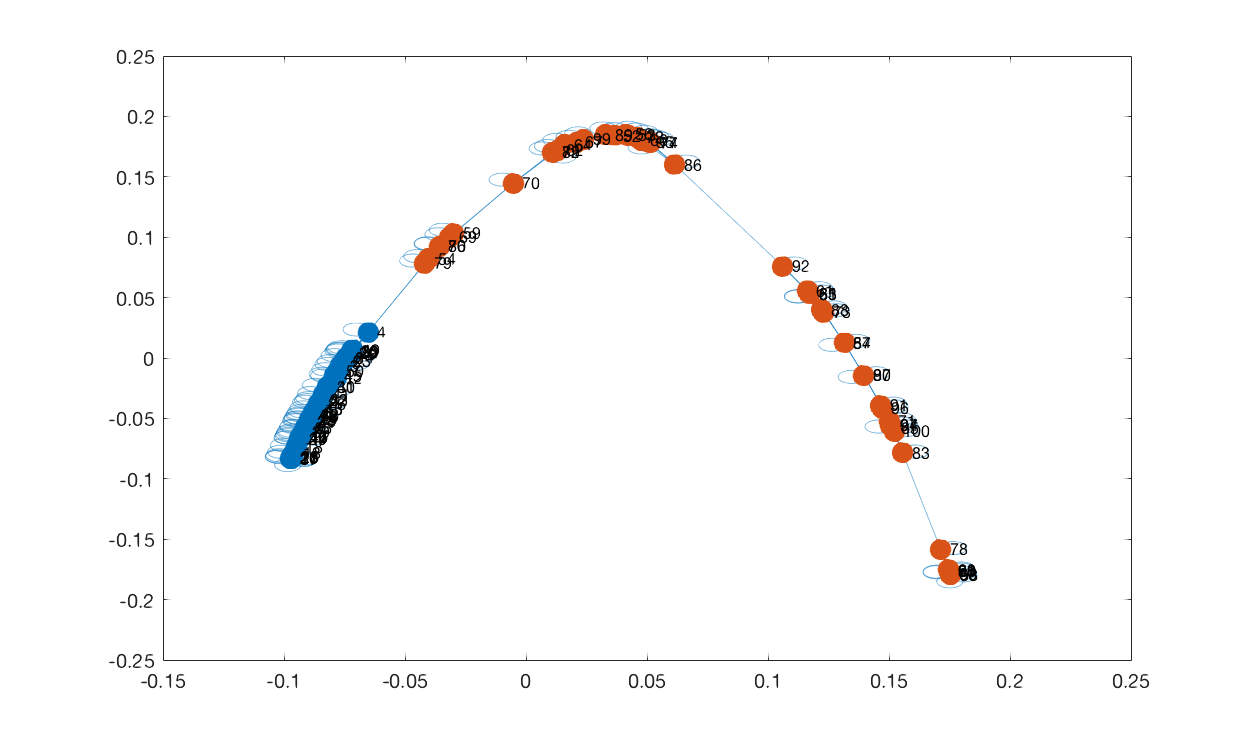
\includegraphics[width=.7\textwidth]{circ3.png}
	\end{center}
\end{frame}

\begin{frame}
	\frametitle{why does this work?}
	Intuitively, since $\bv{v} \in \bv{v}_1, \ldots \bv{v}_k$ are smooth over the graph, 
	\begin{align*}
		\sum_{i,j \in E} (\bv{v}[i] - \bv{v}[j])^2
	\end{align*}
	is small for each coordinate. I.e. this embedding explicitly encourages nodes connected by an edge to be placed in nearby locations in the embedding.
	\begin{center}
		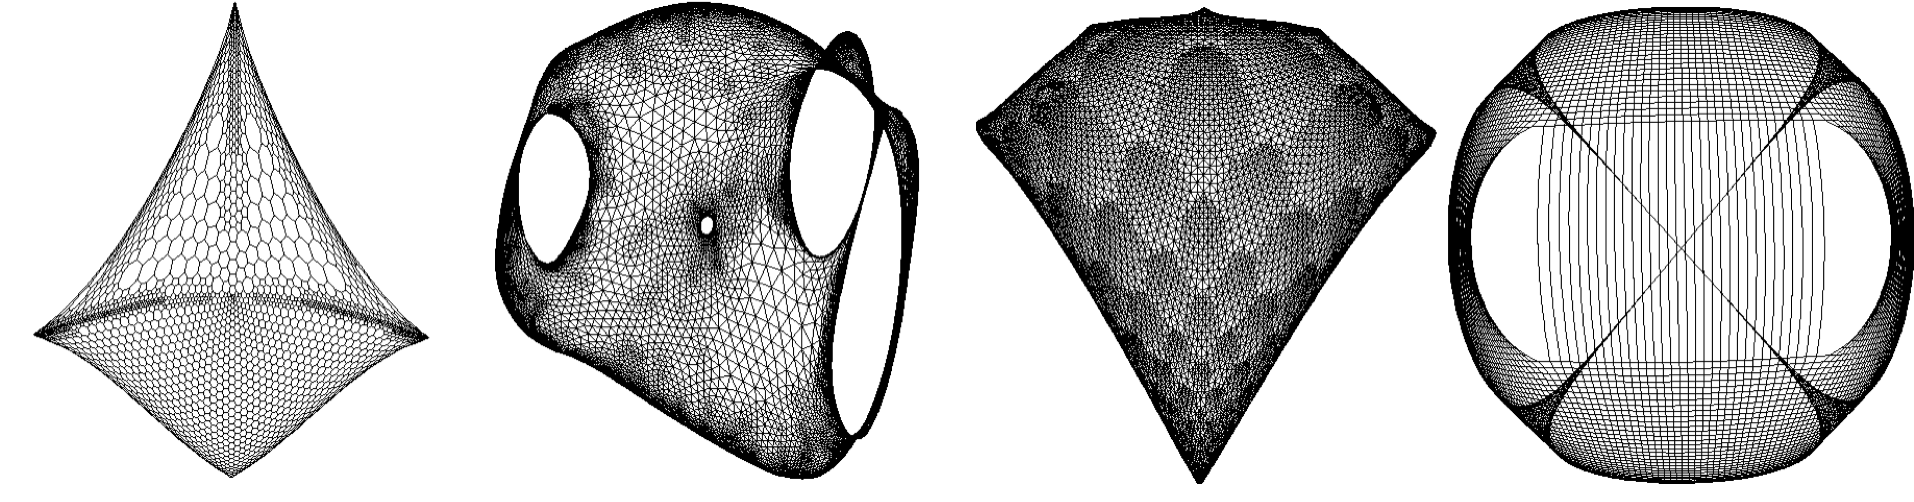
\includegraphics[width=\textwidth]{graph_drawing.png}
		
		Also useful e.g., in graph drawing.
	\end{center}
	
\end{frame}

\begin{frame}
	\frametitle{tons of other applications!}
	Fast balanced partitioning algorithms are also use in distributing data in graph databases, for partitioning finite element meshes in scientific computing (e.g., that arise when solving differential equations), and more. 
	
	\begin{center}
	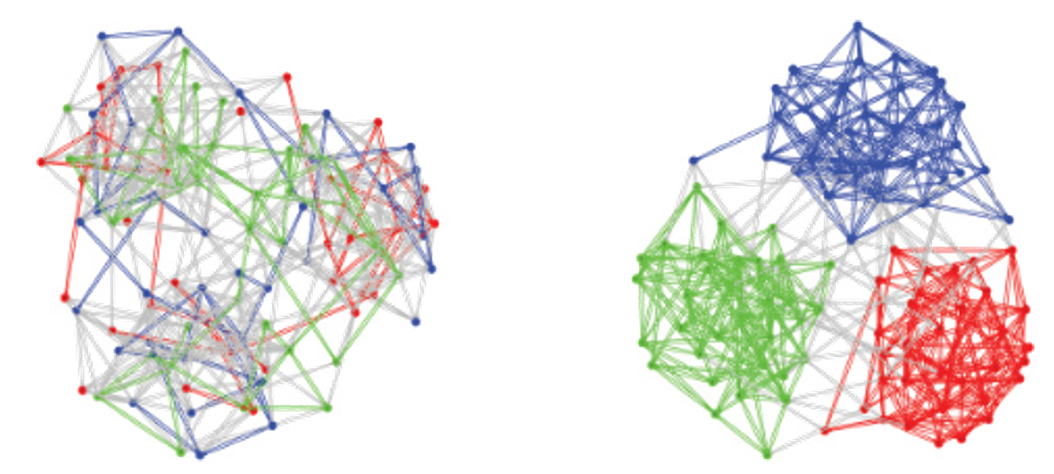
\includegraphics[height=.3\textheight]{balanced_partition.png} \hfill	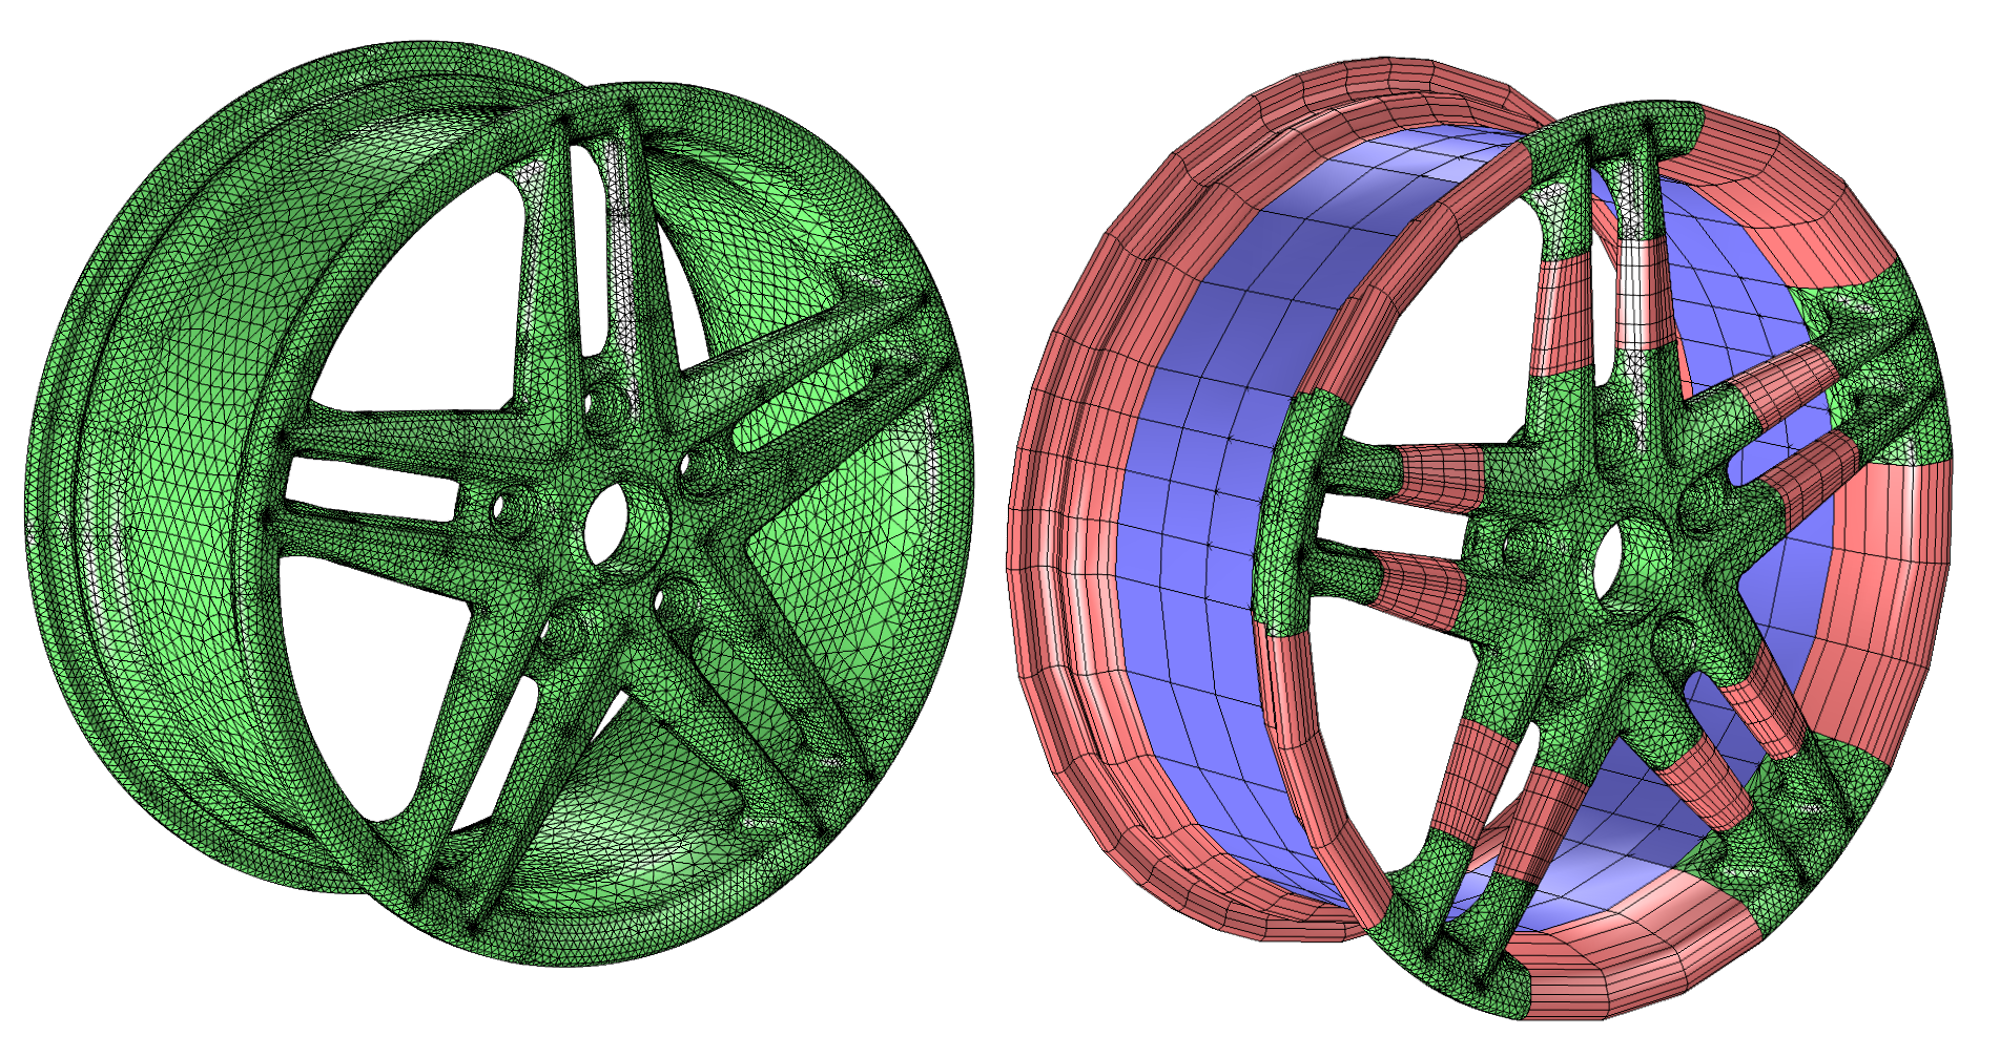
\includegraphics[height=.3\textheight]{finite_element_1.png}
	
	Lots of good software packages (e.g. METIS). 
	\end{center}
\end{frame}

\begin{frame}
	\frametitle{generative models}
	\textbf{So far:} Showed that spectral clustering partitions a graph along a small cut between large pieces.   
	\begin{itemize}
		\item No formal guarantee on the `quality' of the partitioning.
		\item Difficult to analyze for general input graphs.
	\end{itemize}
	\textbf{Common approach:} Design a natural \alert{\textbf{generative model}} that produces \emph{random but realistic} inputs and analyze how the algorithm performs on inputs drawn from this model.
	\begin{itemize}
		\item Very common in algorithm design and analysis. Great way to start approaching a problem.
		\item This is also the whole idea behind Bayesian Machine Learning (can be used to justify $\ell_2$ linear regression, $k$-means clustering, PCA, etc.)
	\end{itemize}
\end{frame}


\begin{frame}[t]
	\frametitle{stochastic block model}
	\begin{center}
		\alert{Ideas for a generative model for \textbf{social network graphs} that would allow us to understand partitioning?}
	\end{center}
	
\end{frame}

\begin{frame}
	\frametitle{stochastic block model}
	\textbf{Stochastic Block Model (Planted Partition Model):} 
	
	Let $G_n(p,q)$ be a distribution over graphs on $n$ nodes, split equally into two groups $B$ and $C$, each with $n/2$ nodes.
	\begin{itemize}
		\item Any two nodes in the \textbf{\alert{same group}} are connected with probability $p$ (including self-loops).
		\item Any two nodes in \textbf{\alert{different groups}} are connected with prob. $q < p$.
	\end{itemize}
	\vspace{-1em}
	\begin{center}
		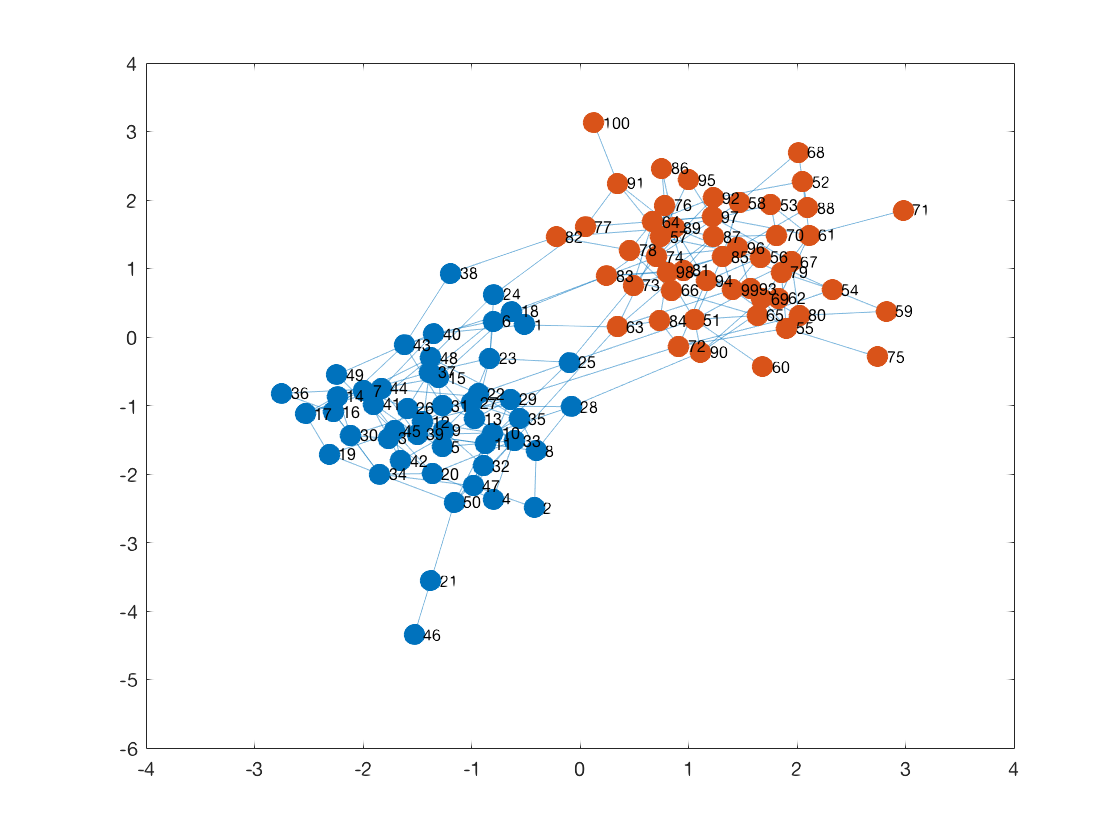
\includegraphics[width=.5\textwidth]{stochasticBlock.png}
	\end{center}
\end{frame}

\begin{frame}{stochastic block model}
	\begin{center}
		Next class we will analyze spectral clustering for SBM graphs.

		Have a good Thanksgiving break!
	\end{center}
\end{frame}

% \frametitle{linear algebraic view}
% 	Let $G$ be a stochastic block model graph drawn from $G_n(p,q)$. 
% 	\begin{itemize}
% 		\item Let $\bv A \in \R^{n \times n}$ be the adjacency matrix of $G$. \alert{What is $\E[\bv A]$?}
% 		\begin{center}
% 			\hspace{-3em}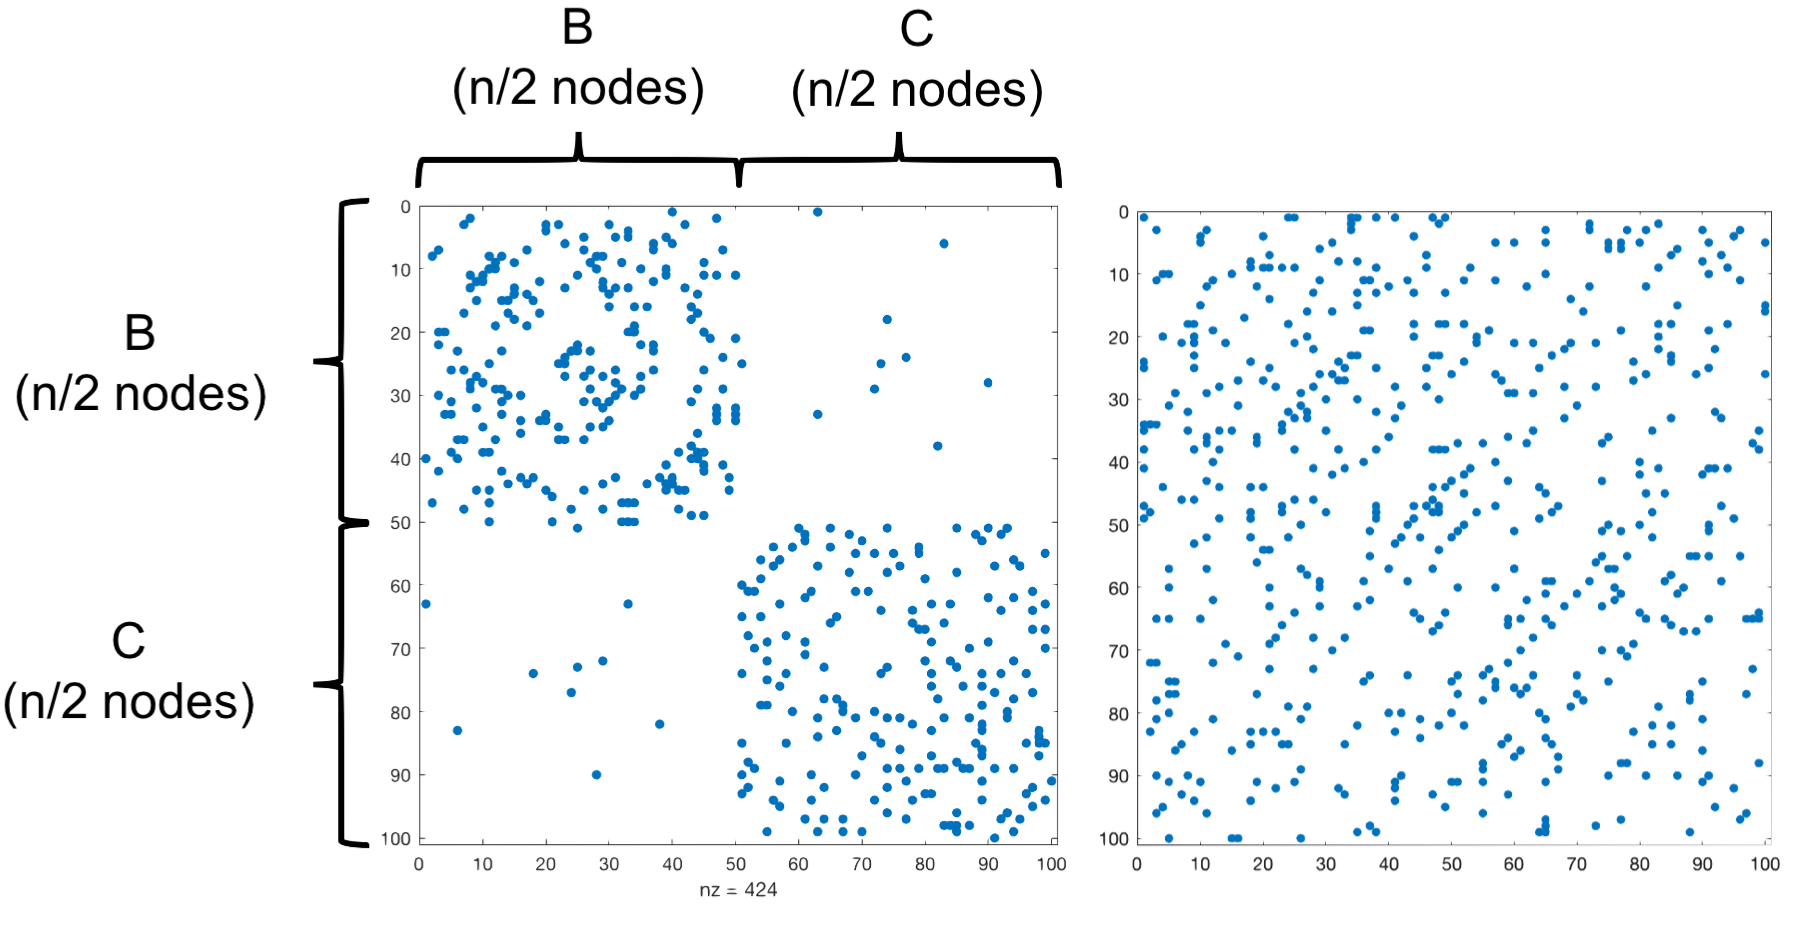
\includegraphics[width=.9\textwidth]{scrambled.png}
% 		\end{center}
% 	\end{itemize}
% \textbf{Note that we are \emph{arbitrarily} ordering the nodes in $\bv{A}$ by group. In reality $\bv{A}$ would look ``scrambled'' as on the right.}
% \end{frame}

% \begin{frame}
% 	\frametitle{expected adjacency spectrum}
% 	Letting $G$ be a stochastic block model graph drawn from $G_n(p,q)$ and $\bv A \in \R^{n \times n}$ be its adjacency matrix. $(\E[\bv A])_{i,j} = p$ for $i,j$ in same group, $(\E[\bv A])_{i,j} = q$ otherwise. 
% 	\begin{columns}
% 		\begin{column}{.6\textwidth}
% 			\begin{center}
% 				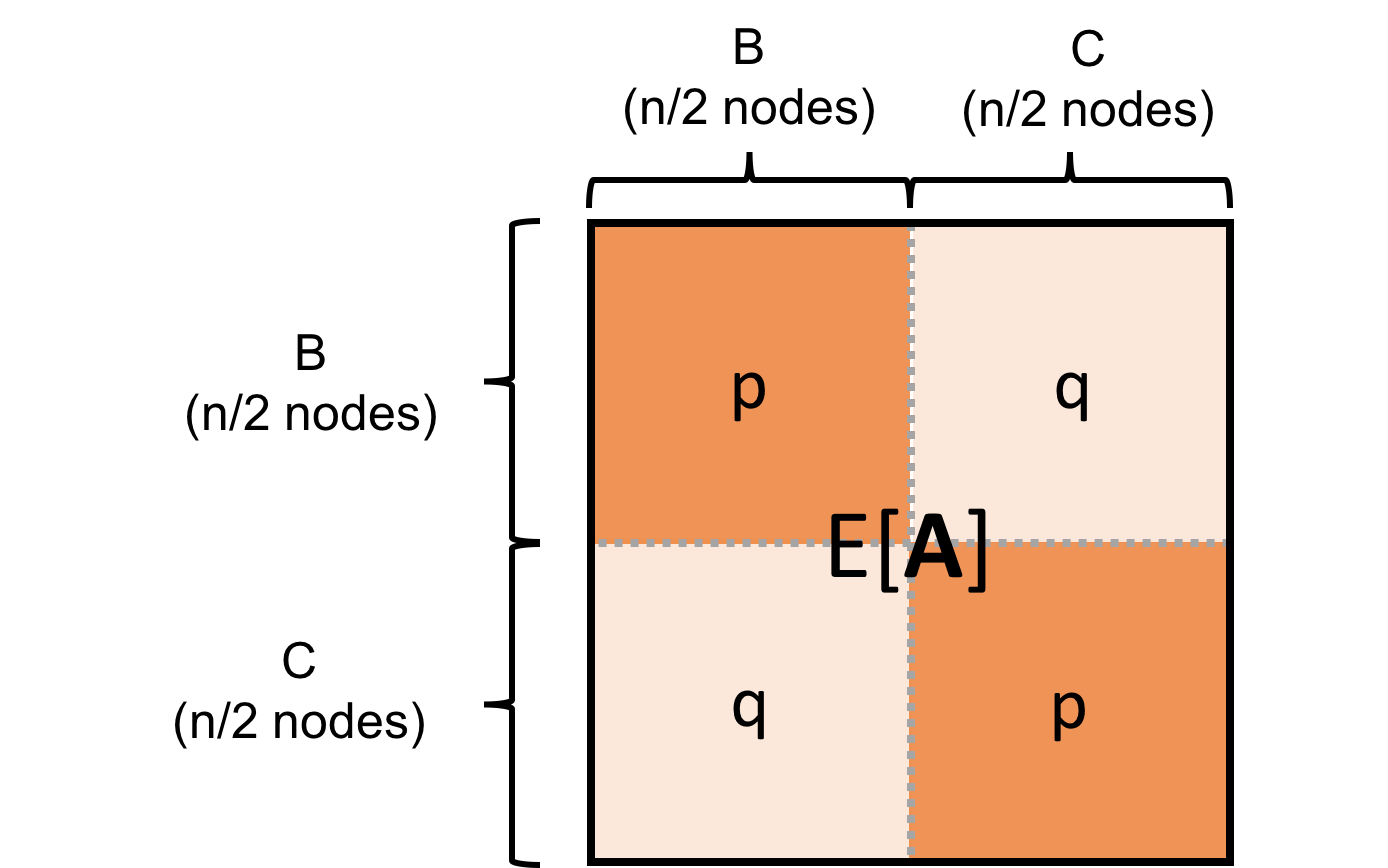
\includegraphics[width=1\textwidth]{expA.png}
% 			\end{center}
% 		\end{column}
% 		\begin{column}{.4\textwidth}
% 			We are going to determine the eigenvectors and eigenvalues of $\E[\bv{A}]$.
% 		\end{column}
% 	\end{columns}
% \end{frame}

% \begin{frame}
% 	\frametitle{expected laplacian}
% 	\begin{center}
% 	What is the expected Laplacian of $G_n(p,q)$?
% 	\vspace{14em}
	
	
% 	$\E[\bv{A}]$ and $\E[\bv{L}]$ have the same eigenvectors and eigenvalues are equal up to a shift/inversion. So second largest eigenvector of $\E[\bv{A}]$ is the same as the second smallest of $\E[\bv{L}]$
% 	\end{center}
% \end{frame}

% \begin{frame}[t]
% 	\frametitle{expected adjacency spectrum}
% 	Letting $G$ be a stochastic block model graph drawn from $G_n(p,q)$ and $\bv A \in \R^{n \times n}$ be its adjacency matrix, what are the eigenvectors and eigenvalues of $\E[\bv{A}]$?
% \end{frame}


% \begin{frame}
% 	\frametitle{expected adjacency spectrum}
% 	\begin{center}
% 		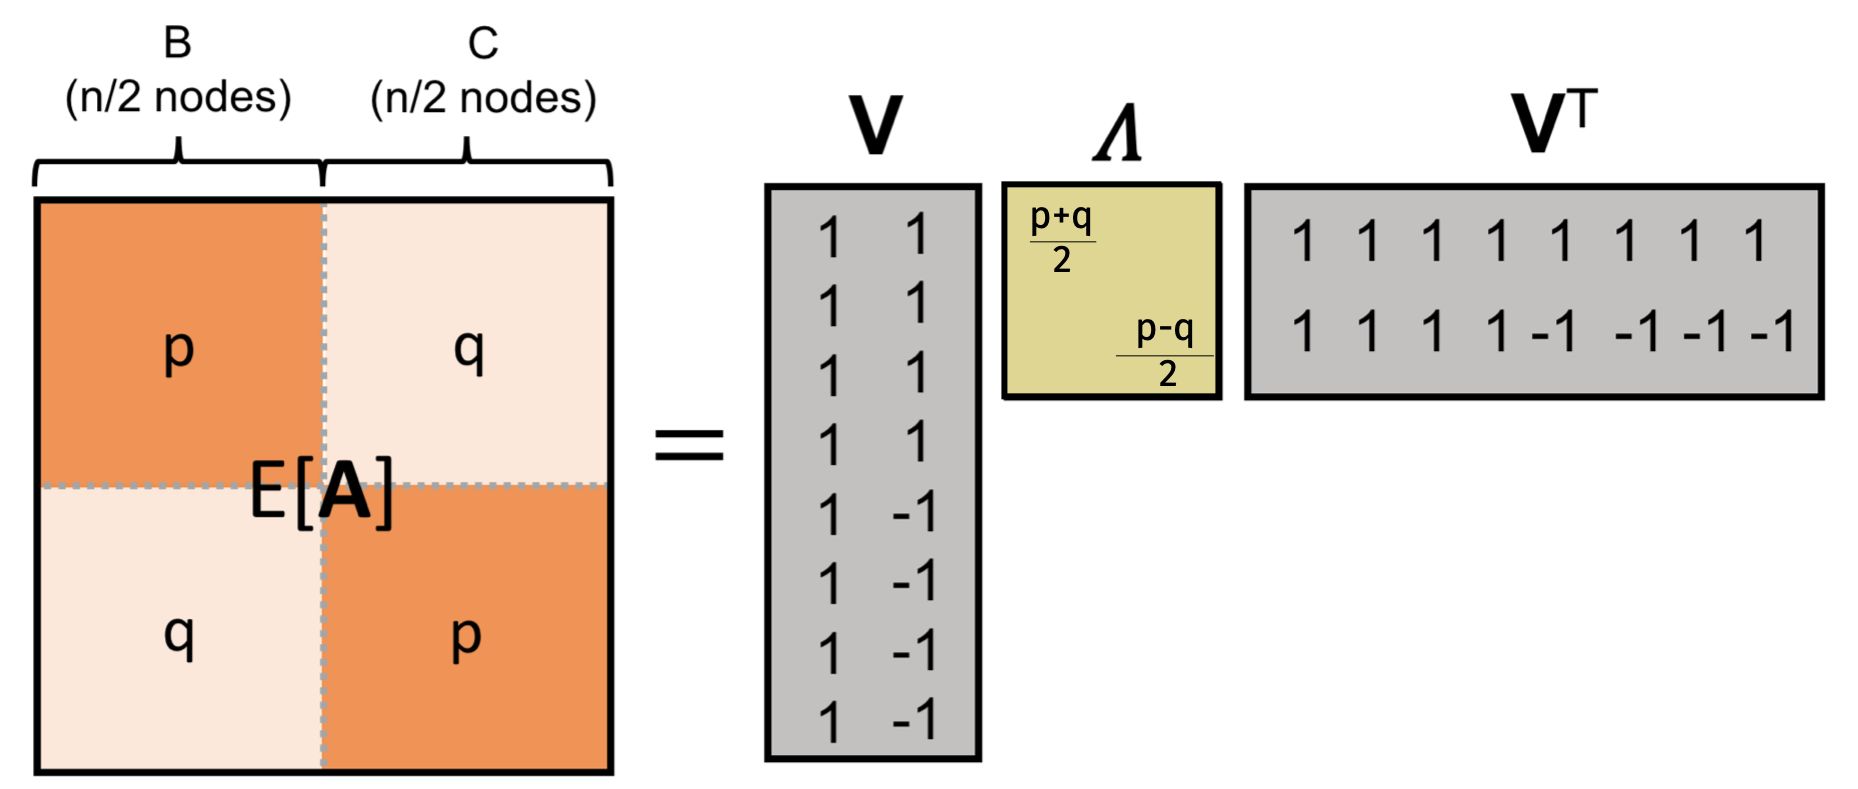
\includegraphics[width=\textwidth]{Aeig_fix.png}
% 	\end{center}
% 	\begin{itemize}
% 		\item $\bv{v}_1 \sim \bv{1}$ with eigenvalue $\lambda_1 = \frac{(p+q) n}{2}$.
% 		\item $\bv{v}_2 \sim \bs{\chi}_{B,C}$ with eigenvalue $\lambda_2 = \frac{(p-q) n}{2}$.
% 		\item $\chi_{B,C}(i) = 1$ if $i \in B$ and $\chi_{B,C}(i) = -1$ for $i \in C$.
% 	\end{itemize}
% 	If we compute $\bv{v}_2$ then we recover the communities $B$ and $C$!
% \end{frame}

% %\begin{frame}[t]
% %	\frametitle{expected laplacian spectrum}
% %	Letting $G$ be a stochastic block model graph drawn from $G_n(p,q)$, $\bv A \in \R^{n \times n}$ be its adjacency matrix and $\bv L$ be its Laplacian, what are the eigenvectors and eigenvalues of $\E[\bv{L}]$?
% %\end{frame}

% \begin{frame}[t]
% 	\frametitle{expected laplacian spectrum}
% 	\textbf{Upshot:} The second smallest eigenvector of $\E[\bv{L}]$, equivalently the second largest of $\E[\bv{A}]$, is $\chi_{B,C}$ -- the indicator vector for the cut between the communities.
% 	\begin{itemize}
% 		\item If the random graph $G$ (equivilantly $\bv{A}$ and $\bv{L}$) were exactly equal to its expectation, partitioning using this eigenvector would exactly recover communities $B$ and $C$.
% 	\end{itemize}
% 	\alert{How do we show that a matrix (e.g., $\bv{A}$) is close  to its expectation?} \textbf{Matrix concentration inequalities.}
% 	\begin{itemize}
% 		\item Analogous to scalar concentration inequalities like Markovs, Chebyshevs, Bernsteins.
% 	\end{itemize}
% \end{frame}

% \begin{frame}
% 	\frametitle{matrix concentration}
% 	\begin{tcolorbox}[colback=green!5,colframe=green!40!black]
% 		\textbf{Matrix Concentration Inequality:}
% 		If $p \ge O \left ( \frac{\log^4 n}{n} \right )$, then with high probability
% 		\begin{align*}
% 			\norm{\bv A - \E[\bv A]}_2 \le O(\sqrt{pn}).
% 		\end{align*}
% 		where $\norm{\cdot}_2$ is the matrix \alert{spectral} norm (operator norm).
% 	\end{tcolorbox}
% 	For $\bv{X} \in \R^{n \times d}$, $\norm{\bv{X}}_2 = \max_{\bv{z}\in\R^d: \norm{\bv{z}}_2 = 1} \norm{\bv X \bv{z}}_2$.
	
% 	For the stochastic block model application, we want to show that the second \emph{eigenvectors} of $\bv{A}$ and $\E[\bv{A}]$ are close. How does this relate to their difference in spectral norm?
% \end{frame}


% \begin{frame}
% 	\frametitle{eigenvector perturbation}
% 	\begin{tcolorbox}[colback=green!5,colframe=green!40!black]
% 		\textbf{Davis-Kahan Eigenvector Perturbation Theorem:}
% 		Suppose $\bv{A},\bv{\overline A} \in \R^{d \times d}$ are symmetric with $\norm{\bv{A}-\bv{\overline A}}_2 \le \epsilon$ and eigenvectors $\bv{v}_1,\bv{v}_2,\ldots, \bv{v}_d$ and $\bar{\bv{v}}_1,\bar{\bv{v}}_2,\ldots, \bar{\bv{v}}v_d$. Letting $\theta(\bv{v}_i,\bar{\bv{v}}_i)$ denote the angle between $\bv{v}_i$ and $\bar{\bv{v}}_i$, for all $i$:
% 		\begin{align*}
% 			\sin \left(\theta(\bv{v}_i,\bar{\bv{v}}_i)\right) \le \frac{\epsilon}{\min_{j \neq i} |\lambda_i - \lambda_j|}
% 		\end{align*}
% 		where $\lambda_1,\ldots,\lambda_d$ are the eigenvalues of $\bv{\overline A}$.
% 	\end{tcolorbox}
% 	The error gets larger if there are eigenvalues with similar magnitudes.
% \end{frame}

% \begin{frame}
% 	\frametitle{eigenvector perturbation}
% 	\begin{center}
% 		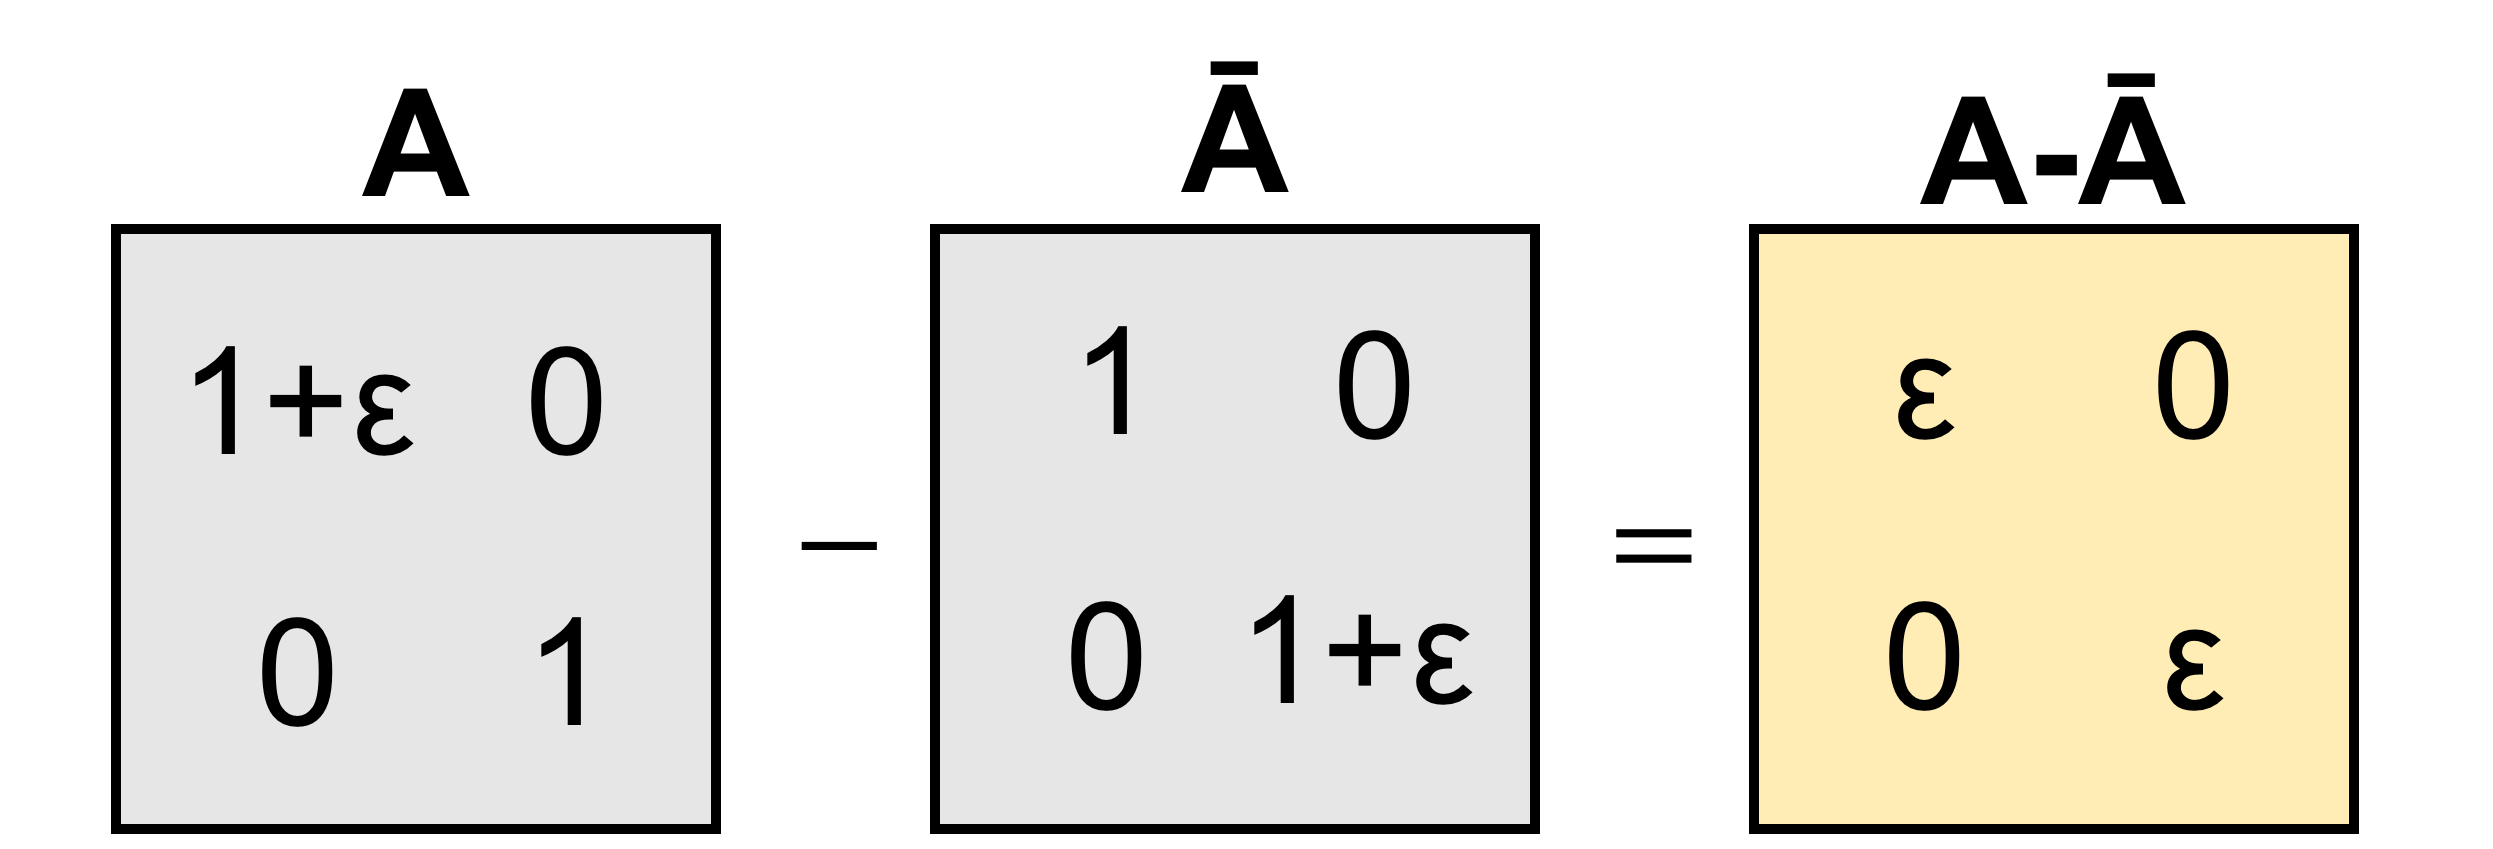
\includegraphics[width=.8\textwidth]{flip.png}
% 	\end{center}
% 	\vspace{13em}
% \end{frame}


% \begin{frame}
% 	\frametitle{application to stochastic block model}
% 	%When $\bv{A}$ is the adjacency matrix of a stochastic block model graph with parameters $p$ and $q$:
% 	%
% 	\small
% 	\textbf{Claim 1 (Matrix Concentration):} For $p \ge O\left (\frac{\log^4 n}{n}\right)$, 
% 	$$\norm{\bv A-\E[\bv{A}]}_2 \le O(\sqrt{pn}).$$
	
% 	\textbf{Claim 2 (Davis-Kahan):} For $p \ge O\left (\frac{\log^4 n}{n}\right)$, 
% 	$$\sin \theta(\bv{v}_2,\bar{\bv{v}}_2) \le \frac{O(\sqrt{pn})}{\min_{j \neq i} |\lambda_i - \lambda_j|} \le \frac{O(\sqrt{p n})}{(p-q)n/2} = \alert{O\left (\frac{\sqrt{p}}{(p-q)\sqrt{n}} \right )}
% 	$$
% 	\textbf{Recall:} $\E[\bv{A}]$, has eigenvalues $\lambda_1 = \frac{(p+q)n}{2}$, $\lambda_2 = \frac{(p-q)n}{2}$, $\lambda_i = 0$ for $i \ge 3$.
% 	\begin{align*}
% 		\min_{j \neq i} |\lambda_i - \lambda_j| = \min \left ({qn}, \alert{\frac{(p-q) n}{2}} \right).
% 	\end{align*}
% 	Assume $\left|\frac{(p-q) n}{2} - 0\right|$ will be the minimum of the two gaps. I.e. smaller than $\left|\frac{(p+q) n}{2} - \frac{(p-q) n}{2}\right| = q n$.
% \end{frame}

% \begin{frame}
% 	\frametitle{application to stochastic block model}
% 	\small
% 	\textbf{So Far:} $\sin \theta(\bv{v}_2,\bar{\bv{v}}_2) \le O\left (\frac{\sqrt{p}}{(p-q)\sqrt{n}} \right )$. What does this give us?
% 	\begin{itemize}
% 		\item Can show that this implies $\norm{\bv{v}_2 - \bar{\bv{v}} v_2}_2^2 \le O\left (\frac{p}{(p-q)^2 n} \right )$ (exercise).
% 		\item $\bar{\bv{v}}_2$ is $\frac{1}{\sqrt{n}} \chi_{B,C}$: the community  indicator vector.
% 		\begin{center}
% 			\vspace{-1em}
% 			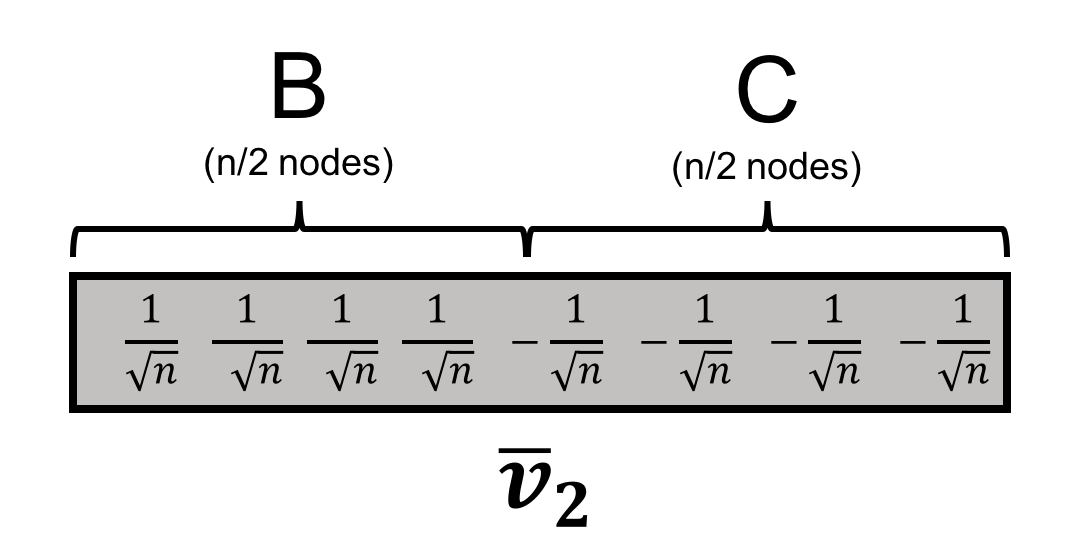
\includegraphics[width=.5\textwidth]{v2.png}
% 		\end{center}
% 		\item Every $i$ where $\bv{v}_2(i)$ and $\bar{\bv{v}}_2(i)$ \alert{differ in sign} contributes $\ge \frac{1}{n}$ to $\norm{\bv{v}_2 - \bar{\bv{v}}_2}_2^2.$
% 		\item So they differ in sign in at most $O \left  (\frac{p}{(p-q)^2}\right )$ positions.
% 	\end{itemize}
% \end{frame}

% %\begin{frame}
% %\frametitle{Matrix Concentration}
% %In scalar concentration bounds we measure distance by the magnitude $|\bv{x} - \E[\bv x]|$. \alert{How should we measure distance in matrix concentration bounds?}
% %\begin{itemize}
% %\item In our stochastic block model application, letting $\hat v_2$ and $v_2$ be the second largest eigenvectors of $\bv{A}$ and $\E[\bv{A}]$ respectively, we want: 
% %\end{itemize}
% %\end{frame}

% \begin{frame}
% 	\frametitle{application to stochastic block model}
% 	\textbf{Upshot:} If $G$ is a stochastic block model graph with adjacency matrix $\bv{A}$, if we compute its second large eigenvector $v_2$ and assign nodes to communities according to the sign pattern of this vector, we will correctly assign all but $O \left  (\frac{p}{(p-q)^2} \right  )$ nodes.
% 	\begin{center}
% 		\vspace{-1em}
% 		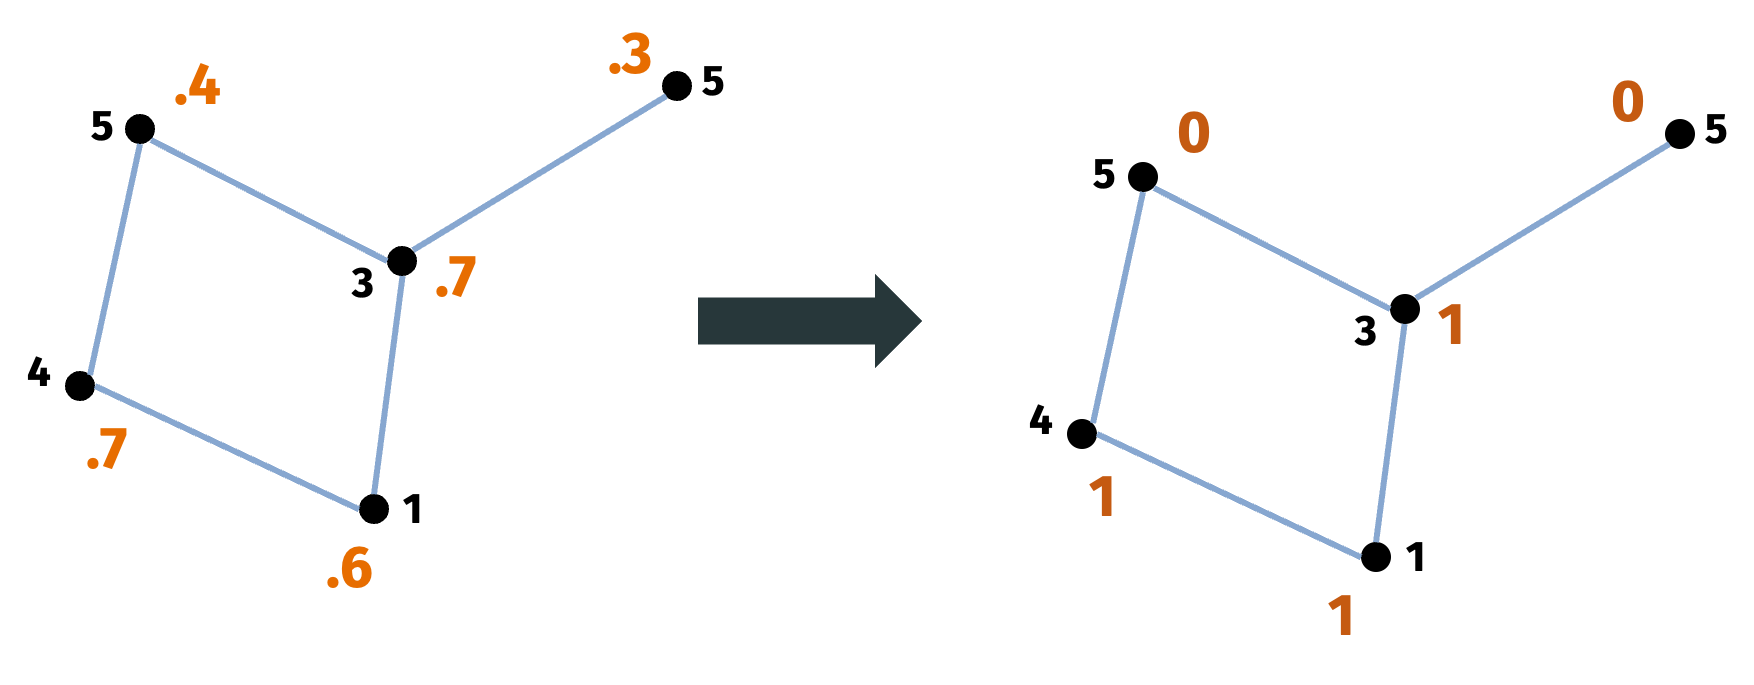
\includegraphics[width=1\textwidth]{round.png}
% 	\end{center}
% 	\begin{itemize}
% 		\item \alert{Why does the error increase as $q$ gets close to $p$?}
% 		\item Even when $p - q = O(1/\sqrt{n})$, assign all but an $O(n)$ fraction of nodes correctly. E.g., assign $99\%$ of nodes correctly.
% 	\end{itemize}
% \end{frame}

% \begin{frame}[t]
% 	\frametitle{randomized numerical linear algebra}
% 	Forget about the previous problem, but still consider the matrix $\bv{M} = \E[\bv{A}]$.
% 	\begin{itemize}
% 		\item Dense $n \times n$ matrix.
% 		\item Computing top eigenvectors takes $\approx O(n^2 / \sqrt{\epsilon})$ time.
% 	\end{itemize}
% 	If someone asked you to speed this up and return \emph{approximate} top eigenvectors, what could you do?
	
% 	\begin{center}
% 		\textbf{\alert{We will discuss this more next class!}}
% 	\end{center}
% \end{frame}

\end{document} 




